\documentclass[11pt]{article}
\usepackage[T1]{fontenc}
\usepackage[utf8]{inputenc}
\usepackage{lmodern}
\usepackage[margin=1.05in]{geometry}
\usepackage{amsmath,amssymb,amsthm,mathtools}
\usepackage{microtype}
\usepackage{enumitem}
\def\DoNotLoadEpstopdf{}
\usepackage{graphicx}
\usepackage{tikz}
\usetikzlibrary{arrows.meta,calc}
\usepackage[hyphens]{url}
\usepackage{hyperref}
\hypersetup{colorlinks=true,linkcolor=blue!45!black,citecolor=blue!45!black,urlcolor=blue!45!black,pdftitle={Quasi-isometric Recognition of Virtually Polycyclic Groups},pdfauthor={OpenAI}}
\setlength{\emergencystretch}{2em}
\setcounter{tocdepth}{2}
\numberwithin{equation}{section}
\newtheorem{theorem}{Theorem}[section]
\newtheorem{proposition}[theorem]{Proposition}
\newtheorem{lemma}[theorem]{Lemma}
\newtheorem{corollary}[theorem]{Corollary}
\theoremstyle{definition}
\newtheorem{definition}[theorem]{Definition}
\newtheorem{remark}[theorem]{Remark}
\newcommand{\R}{\mathbb R}
\newcommand{\Z}{\mathbb Z}
\newcommand{\N}{\mathbb N}
\newcommand{\A}{\mathcal A}
\newcommand{\FP}{\mathrm{FP}}
\DeclareMathOperator{\vol}{vol}
\DeclareMathOperator{\Ad}{Ad}
\DeclareMathOperator{\ad}{ad}
\DeclareMathOperator{\dist}{dist}
\DeclareMathOperator{\supp}{supp}
\DeclareMathOperator{\diam}{diam}
\DeclareMathOperator{\id}{id}
\DeclareMathOperator{\tr}{tr}
\DeclareMathOperator{\GL}{GL}
\DeclareMathOperator{\Hom}{Hom}
\DeclareMathOperator{\Lie}{Lie}
\DeclareMathOperator{\End}{End}
\DeclareMathOperator{\Span}{span}
\DeclareMathOperator{\rank}{rank}
\title{Quasi-isometric Recognition of\\Virtually Polycyclic Groups}
\author{OpenAI}
\date{September 24, 2026}
\begin{document}
\maketitle
\begin{abstract}
We prove that every finitely generated group quasi-isometric to a finitely
generated virtually polycyclic group is virtually polycyclic. This resolves
the lattice-recognition conjecture of Eskin, Fisher and Whyte, which allows
the ambient solvable Lie group in the conclusion to differ from the one in
the hypothesis.
\end{abstract}
\tableofcontents
\section{Introduction}

A group is \emph{polycyclic} if it has a finite subnormal series with cyclic factors. It is \emph{virtually polycyclic} if it contains a polycyclic subgroup of finite index. We prove that virtual polycyclicity can be recognized from the large-scale geometry of a word metric.

A $(K,C)$-\emph{quasi-isometry} $F:X\to Y$, with $K\geq1$ and $C\geq0$, satisfies
\[
 K^{-1}d_X(x,x')-C\leq d_Y(F(x),F(x'))\leq Kd_X(x,x')+C
\]
for all $x,x'\in X$, and every point of $Y$ is within distance $C$ of $F(X)$. Different finite generating sets give quasi-isometric word metrics. 
\begin{theorem}\label{thm:recognition}
Let $P$ be a finitely generated virtually polycyclic group, and let $H$ be any finitely generated group. If $H$ and $P$ are quasi-isometric, then $H$ is virtually polycyclic.
\end{theorem}

The group $H$ in Theorem~\ref{thm:recognition} is subject to no algebraic hypothesis beyond finite generation.

The virtual lattice characterization of polycyclic groups gives the following equivalent formulation. A lattice is a discrete subgroup of finite covolume; it is uniform if the quotient is compact.

\begin{corollary}\label{cor:lattice-recognition}
If a finitely generated group $H$ is quasi-isometric to a lattice in a connected simply connected solvable Lie group, then a finite-index subgroup of $H$ is a uniform lattice in some connected simply connected solvable Lie group.
\end{corollary}

The ambient Lie group in this conclusion may change. The precise lattice statements and finite-index reductions are given in the proof of Corollary~\ref{cor:lattice-recognition}.

\subsection{The recognition problem}

Eskin, Fisher and Whyte formulated the lattice-recognition conjecture
and its equivalent polycyclic formulation in
\cite[Conjecture~1.2 and Remark~(3), p.~929]{EskinFisherWhyte2007}.
Gromov's theorem on groups of polynomial growth settles the virtually
nilpotent case \cite{Gromov1981}. For the full class, Shalom proved that
a finitely generated group quasi-isometric to an infinite polycyclic
group has a finite-index subgroup with infinite abelianization
\cite[Theorem~1.3]{Shalom2004}. The remaining recognition problem asks
for the algebraic structure of an arbitrary finitely generated
comparison group, on which solvability is not assumed.

Height rigidity has been central to the exponential-growth case.
Farb and Mosher formulated horizontal-preservation conjectures for
abelian-by-cyclic models and the recognition conjecture for
$\mathrm{Sol}$ \cite[Section~5]{FarbMosher2000}.
Eskin, Fisher and Whyte established recognition for $\mathrm{Sol}$
by coarse differentiation \cite[Theorem~1.1]{EskinFisherWhyte2013}.
Peng extended this analysis to nondegenerate unimodular split
abelian-by-abelian Lie groups \cite{Peng2011I,Peng2011II}.
Her argument makes local height maps affine and compares them across
boxes; it gives a description of quasi-isometries as well as
virtual-polycyclic recognition
\cite[Theorem~5.3.6 and Corollary~5.3.9]{Peng2011II}.
This class already includes nontrivial Jordan blocks.

For several of these models, height control induces actions on
boundaries, where conjugation theorems give stronger rigidity
conclusions.
Dymarz carried this out for diagonalizable determinant-one models
with no unit-modulus eigenvalues \cite{Dymarz2010}.
Dymarz, Fisher and Xie prove a conjugation theorem for suitable
nilpotent boundaries and apply it to SOL-like groups with possibly
nonabelian nilpotent factors
\cite[Theorems~1.2 and~1.5]{DymarzFisherXie2025}.
Their Section~9 repairs the conjugation step in
\cite[Section~3.3]{Dymarz2010} using amenability. Their recognition
result retains the structural and amenability hypotheses specified
in their Theorem~1.5.

Grayevsky and Pallier obtain rigidity of $\mathrm{Sol}_5$ and its
lattices \cite[Theorem~C]{GrayevskyPallier2025}.
A different strengthening of the geometric hypothesis is commability:
two locally compact groups are commable if they are joined by a finite
zigzag of continuous proper homomorphisms with cocompact image
\cite[Remark~4.C.13]{CornulierDeLaHarpe2016}.
Le Boudec proves virtual-polycyclic recognition under this hypothesis
\cite[Theorem~7 and Corollary~3.7]{LeBoudec2025}.

Theorem~\ref{thm:recognition} resolves recognition for the full class
of virtually polycyclic groups. We establish uniform height control
for the general solvable Lie models described below. Combined with
amenability, this control yields elementary amenability of the
comparison group; finiteness and duality then yield virtual polycyclicity.

\subsection{Uniform bounded height}

We use connected simply connected \emph{real-triangulable} Lie groups: the adjoint representation of their Lie algebra admits a simultaneously upper triangular form over $\R$. Fix a left invariant Riemannian metric on each such group. A group is \emph{unimodular} if its left Haar measure is also right invariant. The relevant quotient has a canonical definition.

\begin{definition}\label{def:canonical-height}
Let $\mathfrak g$ be the Lie algebra of a real-triangulable group $G$. Denote the diagonal characters of a simultaneous real triangular form of $\ad$ by $\chi_1,\ldots,\chi_s$, including repetitions and zero characters. Put
\[
 \mathfrak k=\bigcap_{j=1}^s\ker\chi_j,
 \qquad W=\mathfrak g/\mathfrak k.
\]
The \emph{exponential height map} is the homomorphism $\pi:G\to(W,+)$ whose differential is the quotient map.
\end{definition}

For the zero-dimensional algebra, the empty intersection is $\mathfrak g$. The characters vanish on $[\mathfrak g,\mathfrak g]$, so the quotient is abelian. Their multiset is intrinsic to the adjoint representation; hence $\mathfrak k$ is independent of the triangular basis. Simple connectedness gives the homomorphism $\pi$. Fix any norm on $W$.

\begin{theorem}[Uniform bounded height]\label{thm:bounded-height}
Let $G$ be a connected simply connected real-triangulable unimodular Lie group, with a fixed left invariant Riemannian metric, exponential height map $\pi:G\to W$, and a fixed norm on $W$. There is a finite subgroup $\A_G\leq\GL(W)$ such that, for every $K\geq1$ and $C\geq0$, there is a constant $B=B(G,K,C)$ with the following property. Every $(K,C)$ self quasi-isometry $F$ of $G$ has an $A_F\in\A_G$ satisfying
\begin{equation}\label{eq:height-main}
 \bigl\|\pi F(g)-\pi F(1)-A_F\pi(g)\bigr\|\leq B
 \qquad(g\in G).
\end{equation}
\end{theorem}

The finite group $\A_G$ will be constructed from the exponential rates of bracket-generated volume in Lemma~\ref{lem:support-symmetries}. It depends on $G$, whereas the error bound depends additionally on the quasi-isometry constants. When $W=0$, the height statement is vacuous and $G$ is nilpotent; this case is treated separately in recognition.

\subsection{How height gives recognition}

We first explain how Theorem~\ref{thm:bounded-height} implies recognition; the complete deduction appears in Section~\ref{sec:recognition}. A virtually polycyclic group is quasi-isometric to a connected simply connected real-triangulable unimodular Lie model $G$. Transporting the left translation action of $H$ across a quasi-isometry gives maps of $G$ with uniform quasi-isometry bounds that respect multiplication up to a uniformly bounded error. This is a \emph{uniform quasi-action}. Equation~\eqref{eq:height-main} assigns a linear part in the finite group $\A_G$ to each element of $H$. After passing to a finite-index subgroup $H_0$, all linear parts are the identity. The group $H$ inherits amenability from its virtually polycyclic comparison group by quasi-isometry. Amenability then corrects the bounded defect in the height translations to a homomorphism $\tau:H_0\to W$.

Every finitely generated subgroup of $\ker\tau$ has polynomial growth: its word paths have bounded height, and the volume of possible endpoints grows polynomially. Gromov's theorem makes each such subgroup virtually nilpotent. Thus $\ker\tau$, and consequently $H$, is elementary amenable. Finiteness properties and Poincar\'e duality inherited from the comparison group, together with the structure of elementary amenable groups, then imply that a finite-index subgroup of $H$ is polycyclic. The bounded error is essential: a sublinear height bound alone would not give the bounded-height word paths used to prove polynomial growth in the kernel.

\subsection{The height argument}

The geometric meaning of height is already visible in
$\mathrm{Sol}=\R^2\rtimes\R$, where $t\in\R$ acts on the two coordinate
directions by $e^t$ and $e^{-t}$.  A bounded horizontal move at height $t$
can change the first coordinate by order $e^t$ and the second by order
$e^{-t}$.  To reach many endpoints, a path can make its first-coordinate
move high up and its second-coordinate move low down.  If its allowed
heights form $r[a,b]$, the resulting rectangle has area of order
$e^{r(b-a)}$.  Thus the height range determines an exponential rate of
accessible volume.

For a general Lie model, the corresponding rate is a function $P(E)$ of
the compact convex allowed height set $E\subset W$.  Its definition in
Section~\ref{sec:boxes} includes every bracket direction generated by the
expanding directions.  Paths of length $O(r)$ from one starting point,
visiting the appropriate support positions and returning to a common
height, reach
$e^{rP(E)+o(r)}$ endpoints separated at a fixed scale.  Their images also have length
$O(r)$.  If those images remain at heights in $rE'$ up to sublinear
errors, the image paths can
reach at most $e^{rP(E')+o(r)}$ separated endpoints.  A quasi-isometry
therefore forces $P(E)\le P(E')$.  Applying this comparison in both
directions will restrict an affine height slope to the finite group
$\mathcal A_G$.

The proof must first produce such slopes and then make them independent
of the averaging, chart, and scale used to find them.  Choose the
nilpotent groups $N,D$ of Section~\ref{sec:models}, with $N$ normal and
$G=ND$.  The expression $g=nd$ need not be unique.  We study the height
function on the sets $xnD$: for fixed $x\in G$ and $n\in N$, rescale
$d\mapsto\pi F(xnd)$ on larger and larger intrinsic $D$-balls.  These are
the $D$-charts, or sheets indexed by $n$.  Endpoint counts instead use
the slices $xNd$ at a fixed $D$-position, where the parameterization by
$N$ is injective.

The geometric proof has three stages. First we study a compact space of
normalized quasi-isometries: each map is translated so that it sends the
identity to the identity. Moving the basepoint and recentering defines
an action on this space. This construction follows Shalom's
measured-coupling viewpoint \cite[Sections~2.1--2.2]{Shalom2004}.
For each ergodic invariant probability measure, the reduced-cohomology
vanishing theorem of Cornulier and Tessera
\cite[Corollary~1.9]{CornulierTessera2020} supplies a linear height slope.
The volume comparison above restricts this slope to $\mathcal A_G$ once
it is applied to the map and its inverse. For the reverse comparison we
need the inverse of the same slope; a coupling constructed from Haar
measure provides it.

Second we pass from invariant measures to arbitrary maps. We sample
large $D$-charts and rescale their height functions. Stationary
increments constrain each limiting profile, while accessible endpoint
volume prevents it from folding. Together these facts make every
supported limiting profile affine on the chart interior. The volume
argument still works after restricting the switch parameters to a set
retaining a subexponential fraction of their measure: a polynomial-image estimate retains the
required exponential endpoint volume.
Different sheets could nevertheless have different affine maps.
If neighboring profiles had different linear parts, a limiting
comparison at supporting heights would force a suitable source height
segment to have opposite target directions on the two sheets.
Alternating moves on the sheets would then produce a target volume
exponent twice the source exponent, contradicting the volume comparison.
Haar multipliers in suitable nilpotent
quotients then detect, and eliminate, differences of their translations.
Comparison across scales and basepoints gives one global slope with
a uniform sublinear error.

Finally we improve this error to a bounded one. Contracting rays define
maps between nilpotent quotient boundaries. The Haar volumes of their
images record height; averaging translated sets then bounds its error.
Boundary conjugation theorems, such as those in
\cite{Dymarz2010,DymarzFisherXie2025}, produce rigid actions from height
control. Here, starting from the uniform sublinear estimate, the
boundary maps bound the remaining height error through their image
measures. The recognition argument can then use
the bounded-height kernel and the finiteness and duality theorems.

The progression from weak height control to bounded error, followed by
an application to a transported group action, already occurs in
\cite[Sections~6.1--6.2 and Theorem~7.3]{EskinFisherWhyte2012}.
The present proof establishes the estimate for the full class in
Theorem~\ref{thm:bounded-height}. Its volume calculations retain both
the bracket directions in $N$ and the multiplicity of the surjection
$N\rtimes D\to G$, so no complementary height subgroup is required.

Sections~\ref{sec:models}--\ref{sec:polynomial-volume} develop the Lie
coordinates, volume estimates, and restricted-product lemma.
Section~\ref{sec:stationary} identifies stationary slopes. The profile
and neighboring-chart arguments lead to the uniform sublinear estimate
in Section~\ref{sec:uniformity}; Section~\ref{sec:boundary} proves bounded
height. Section~\ref{sec:recognition} completes the group-theoretic
deduction.

\section{Cartan models and the canonical height}
\label{sec:models}

Throughout this section, $G$ is a connected, simply connected,
real-triangulable, unimodular Lie group, with Lie algebra $\mathfrak g$.
We fix left invariant Riemannian metrics on every group under consideration.
The notation $|x|_J$ denotes distance from the identity in the intrinsic
metric of $J$. We construct nilpotent groups $N,D$ whose multiplication
maps onto $G$, identify their height coordinates with the canonical quotient
of Definition~\ref{def:canonical-height}, and establish the polynomial
coordinate estimates needed to retain the nonsemisimple parts of the
adjoint action.

The fixed metrics are complete. Indeed, choose a relatively compact identity
neighborhood containing a metric ball of positive radius. A Cauchy
sequence eventually lies in one left translate of that ball, hence in
a compact set; a convergent subsequence then forces the whole sequence
to converge. By the Hopf--Rinow theorem, closed bounded sets are compact
and any two points can be joined by a minimizing geodesic.

\subsection{The Cartan decomposition and its multiplication map}

A Cartan subalgebra of a solvable Lie algebra is a nilpotent,
self-normalizing subalgebra.  Choose one, denoted by $\mathfrak d$.
For a real character $\gamma:\mathfrak d\to\R$, its generalized weight
space in $\mathfrak g$ is
\[
 \mathfrak g_\gamma
 =\{u\in\mathfrak g:
   (\ad(v)-\gamma(v)\id)^{\dim\mathfrak g}u=0
   \text{ for every }v\in\mathfrak d\}.
\]
Only characters with a nonzero space are called weights.  The exponent
in this definition can be replaced by any sufficiently large fixed integer.
In particular, this definition allows a nilpotent part on each weight
space and does not require $\mathfrak d$ to be abelian.

\begin{lemma}[Cartan model]\label{lem:cartan-model}
There is a real generalized weight decomposition
\begin{equation}\label{eq:cartan-weight-decomposition}
 \mathfrak g=\bigoplus_\gamma\mathfrak g_\gamma,
 \qquad \mathfrak g_0=\mathfrak d,
 \qquad
 [\mathfrak g_\gamma,\mathfrak g_\eta]
       \subseteq\mathfrak g_{\gamma+\eta}.
\end{equation}
Let $\mathfrak n$ be the subalgebra generated by the spaces with nonzero
weight.  Then $\mathfrak n$ is a nilpotent ideal contained in
$[\mathfrak g,\mathfrak g]$, and $\mathfrak g=\mathfrak n+\mathfrak d$.
There are homogeneous generators $X_1,\ldots,X_\nu$ of $\mathfrak n$ whose
images form a basis of $\mathfrak n/[\mathfrak n,\mathfrak n]$ and whose
weights $\alpha_1,\ldots,\alpha_\nu$ are all nonzero.

The groups $N=\exp_G(\mathfrak n)$ and $D=\exp_G(\mathfrak d)$ are closed
and simply connected, and $N$ is normal in $G$.  With the conjugation
action of $D$ on $N$, multiplication defines a surjective Lie homomorphism
and submersion
\begin{equation}\label{eq:cartan-multiplication}
 q:N\rtimes D\longrightarrow G,\qquad q(n,d)=nd.
\end{equation}
Its kernel is
\begin{equation}\label{eq:cartan-overlap-kernel}
 \ker q=\{(a^{-1},a):a\in N\cap D\}.
\end{equation}
Moreover, $N\cap D=\exp_G(\mathfrak n\cap\mathfrak d)$.
Every compact subset of $G$ has lifts in a compact subset of $N\rtimes D$.
Finally, $N=1$ if and only if $G$ is nilpotent.
\end{lemma}

\begin{proof}
We give the decomposition argument to specify precisely which parts of
the Cartan action may be nonsemisimple; see also
\cite[Section~4.D]{CornulierTessera2017} for the Cartan grading.
For $v,u\in\mathfrak d$, nilpotence of $\mathfrak d$ gives
\[
 (\ad_{\End(\mathfrak g)}(\ad v))^b(\ad u)
   =\ad((\ad v)^b u)=0
\]
for sufficiently large $b$.  Consequently $\ad u$ preserves every
generalized eigenspace of $\ad v$.  Indeed, between two primary blocks
with distinct eigenvalues, the commutator with $\ad v$ is invertible,
so an operator killed by a power of that commutator has no such block.
All eigenvalues are real by real triangulability.  Successively taking
the primary decompositions for a basis of $\mathfrak d$ therefore gives
simultaneous invariant primary spaces.  On each such space all diagonal
entries of a triangular representation agree on that basis, and hence
agree as linear forms on $\mathfrak d$.  Their common form $\gamma$ is a
character, since diagonals of commutators vanish.  This proves the direct
sum decomposition into the spaces in
\eqref{eq:cartan-weight-decomposition}.

The derivation identity shows that weights add under brackets: applying
$\ad v-(\gamma(v)+\eta(v))\id$ repeatedly to $[x,y]$, with
$x\in\mathfrak g_\gamma$ and $y\in\mathfrak g_\eta$, gives a binomial
sum involving powers of $\ad v-\gamma(v)\id$ on $x$ and of
$\ad v-\eta(v)\id$ on $y$.  Every summand vanishes at a sufficiently
large power.  Nilpotence of $\mathfrak d$ gives
$\mathfrak d\subseteq\mathfrak g_0$.  If this inclusion were strict,
the induced action of $\mathfrak d$ on $\mathfrak g_0/\mathfrak d$
would consist of nilpotent operators.  Engel's theorem would give a
nonzero fixed class.  Any representative of that class normalizes
$\mathfrak d$, contrary to self-normalization.  Thus
$\mathfrak g_0=\mathfrak d$.

The nonzero weight spaces are $\mathfrak d$-invariant.  Their generated
subalgebra $\mathfrak n$ is therefore $\mathfrak d$-invariant, and
$\mathfrak g=\mathfrak n+\mathfrak d$ makes it an ideal.  If
$\gamma\ne0$, choose $v\in\mathfrak d$ with $\gamma(v)\ne0$.
The restriction of $\ad v$ to $\mathfrak g_\gamma$ is invertible, so
$\mathfrak g_\gamma\subseteq[\mathfrak g,\mathfrak g]$.
In a simultaneous real triangularization of $\ad(\mathfrak g)$,
every element of $\ad([\mathfrak g,\mathfrak g])$ is strictly upper
triangular.  Engel's theorem applied to the derived algebra proves
its nilpotence, and hence that of $\mathfrak n$.

The images of the generating nonzero weight spaces span
$\mathfrak n/[\mathfrak n,\mathfrak n]$, and its induced weight
decomposition has no zero summand.  Choose a homogeneous basis of this
quotient and homogeneous lifts $X_i$.  These lifts generate
$\mathfrak n$: if $\mathfrak h$ is their generated subalgebra and
$\mathfrak n^j$ denotes the lower central series, then
$\mathfrak n=\mathfrak h+\mathfrak n^2$.  Induction, using brackets,
gives $\mathfrak n=\mathfrak h+\mathfrak n^j$ for every $j$, and
nilpotence concludes the argument.

We now pass from Lie algebras to groups. Dixmier's real-root criterion implies that
$\exp_G:\mathfrak g\to G$ is an analytic diffeomorphism
\cite[Theorem~3]{Dixmier1957}.  The inclusion of either nilpotent
subalgebra integrates from its simply connected Baker--Campbell--Hausdorff
group, and this homomorphism is the restriction of $\exp_G$ in
exponential coordinates.  It is injective, with closed image, because
$\exp_G$ is a diffeomorphism and each subalgebra is a closed vector
subspace.  Injectivity of $\exp_G$ also gives the stated description
of $N\cap D$.  This proves the claims about $N,D$, including normality
of $N$.

The group law in the domain of $q$ is
\[
 (n,d)(n',d')=(n(dn'd^{-1}),dd'),
\]
which verifies the homomorphism assertion.  Its derivative at the
identity is $(x,v)\mapsto x+v$, which is onto.  Its image is therefore
an open subgroup of the connected group $G$, so it is all of $G$;
translation also makes $q$ a submersion everywhere.  The kernel formula
follows directly from $nd=1$.  Local smooth sections of a submersion,
restricted to relatively compact neighborhoods, give compact sets of
lifts; a finite cover proves the claim for an arbitrary compact set.

If $\mathfrak n=0$, then $\mathfrak g=\mathfrak d$ is nilpotent.
Conversely, in a nilpotent $\mathfrak g$ all adjoint operators are
nilpotent.  The decomposition just proved then has only weight zero,
so $\mathfrak g=\mathfrak d$ and $\mathfrak n=0$.
\end{proof}

The map $q$ will let us estimate paths using a nilpotent $D$ coordinate.
Its kernel in \eqref{eq:cartan-overlap-kernel} is retained throughout;
the argument does not require a complementary subgroup to $N$.
To control conjugation by a $D$ element of intrinsic length $O(r)$,
we need polynomial bounds on its logarithmic coordinates. We establish
those bounds next, together with the rescaling of $D$ used for large charts.

\subsection{Intrinsic coordinates and the graded Cartan limit}

Write $\mathfrak d^1=\mathfrak d$ and
$\mathfrak d^{j+1}=[\mathfrak d,\mathfrak d^j]$ for the lower central
series.  Choose vector subspaces $V_j$ such that
\begin{equation}\label{eq:d-filtration-splitting}
 \mathfrak d=V_1\oplus\cdots\oplus V_s,
 \qquad \mathfrak d^j=V_j\oplus\cdots\oplus V_s.
\end{equation}
Thus $V_1$ represents $V=\mathfrak d/[\mathfrak d,\mathfrak d]$.
Fix Euclidean norms on these spaces.  Define
$\delta_r(\sum_j v_j)=\sum_j r^jv_j$ for $r>0$.  The associated
graded bracket on the same vector space is given, for $v_i\in V_i$
and $v_j\in V_j$, by
\[
 [v_i,v_j]_\infty=\operatorname{pr}_{i+j}[v_i,v_j].
\]
Here $\operatorname{pr}_k=0$ for $k>s$.
Let $D_\infty$ be its simply connected nilpotent group and set
\begin{equation}\label{eq:d-delta-definition}
 \Delta_r(\exp_\infty v)=\exp_D(\delta_r v).
\end{equation}
When $D=1$, take $s=1$ and $V_1=0$; the assertions below are immediate.

These weighted coordinates and graded limits belong to the classical
large-scale geometry of nilpotent groups; see
\cite{Guivarch1973,Pansu1983}. The maps $\Delta_r$ will let us place
growing $D$-charts on the fixed domain $D_\infty$. We give the finite
Baker--Campbell--Hausdorff estimates needed here.

\begin{lemma}[Nilpotent coordinates and scaling]\label{lem:d-scaling}
There is a constant $C\ge1$, depending only on $D$, the metric, and the
splitting, such that for $d=\exp_D(\sum_jv_j)$,
\begin{align}
 \|v_j\|&\le C(1+|d|_D)^j \quad(1\le j\le s),
       \label{eq:d-coordinate-upper}\\
 |d|_D&\le C\left(1+\max_{1\le j\le s}\|v_j\|^{1/j}\right).
       \label{eq:d-coordinate-reverse}
\end{align}
The group laws transported from $D$ by $\Delta_r$ converge, with all
derivatives on compact coordinate sets, to the law of $D_\infty$ as
$r\to\infty$.  Every compact $K\subset D_\infty$ satisfies
$\sup_{z\in K}|\Delta_r z|_D=O_K(r)$ for $r\ge1$.
Conversely, for every fixed $C_0$, all
$\Delta_r^{-1}\{d:|d|_D\le C_0r\}$, $r\ge1$, lie in one compact
coordinate set.
If $z_r,z'_r$ belong to a fixed compact coordinate set and their coordinate
difference tends to zero, then
\begin{equation}\label{eq:d-scaling-equicontinuity}
 \dist_D(\Delta_r z_r,\Delta_r z'_r)=o(r).
\end{equation}
For $v\in V_1$ one also has
\begin{equation}\label{eq:d-horizontal-flow-limit}
 \Delta_r^{-1}\bigl(\Delta_r z\exp_D(rt v)\bigr)
     \longrightarrow z\exp_\infty(tv),
\end{equation}
uniformly when $z,t,v$ range over fixed compact sets.
Haar measures on $D$ and $D_\infty$ are Lebesgue measure in these
exponential coordinates, up to fixed scalars.  If both scalars are
chosen equal and $Q=\sum_jj\dim V_j$, then $\Delta_r$ multiplies Haar
volume by $r^Q$, and
\begin{equation}\label{eq:d-polynomial-volume}
 c t^Q\le \vol_D\{d:|d|_D\le t\}\le C t^Q \qquad(t\ge1)
\end{equation}
for some $c>0$.  In particular $D$ has doubling Haar measure:
\begin{equation}\label{eq:nilpotent-doubling}
 \vol_D B_D(1,2t)\le C\vol_D B_D(1,t)\qquad(t>0).
\end{equation}
Every conclusion of this lemma holds for an arbitrary connected,
simply connected nilpotent Lie group $L$ equipped with a left invariant
Riemannian metric and a splitting of its lower central filtration,
with $L$ in place of $D$ and constants allowed to depend on $L$.
\end{lemma}

\begin{proof}
We first bound the coordinates of a short path. For the reverse estimate,
we construct uniformly bounded products of degree-one exponentials in
the rescaled groups. The remaining assertions follow from these
coordinates and the Haar Jacobian.

A path of length at most $t$ splits its endpoint into a product of
at most $C(1+t)$ increments from a fixed compact neighborhood.  Their
logarithms lie in a fixed bounded set.  In a product of $a$ exponentials,
the degree-$b$ part of its formal logarithm has a sum of absolute
coefficients at most $C_b(1+a)^b$.  To see the bound, expand the product
of formal exponentials through degree $s$ in the noncommuting variables,
and then use the finite expansion of $\log(1+u)$ in those degrees.
The degree-$b$ coefficient sum of the product is at most $a^b/b!$;
the finitely many compositions of $b$ appearing in the logarithm give
the asserted bound.  Applying the degree-$b$ Dynkin projection, which
sends an associative monomial to its iterated bracket and acts by
multiplication by $b$ on homogeneous Lie polynomials, converts this
expansion to brackets with only a degree-dependent coefficient bound.
A bracket involving more than $j$ increments belongs to
$\mathfrak d^{j+1}$ and has zero $V_j$ projection.  Evaluating the
remaining finitely many types of brackets on the bounded logarithms
therefore bounds this projection by $C_j(1+a)^j$.  This proves
\eqref{eq:d-coordinate-upper}.

For the converse, we first record the limit of the transported laws.
The inclusion
$[V_i,V_j]\subseteq\bigoplus_{k\ge i+j}V_k$ shows that the coefficient
of a bracket from $V_i\times V_j$ into $V_k$, when transported by
$\delta_r$, is multiplied by $r^{i+j-k}$.  For $r\ge1$ these
coefficients are bounded and converge to the associated graded bracket.
The finite Baker--Campbell--Hausdorff formula proves convergence of the
group laws and all their derivatives on compact sets.  Denote the
transported group by $D_r$; its underlying exponential coordinate space
is the fixed vector space $\bigoplus_jV_j$.

We now produce uniformly bounded products of degree-one exponentials
covering a fixed coordinate neighborhood.  Choose a basis
$e_1,\ldots,e_a$ of $V_1$.  These vectors generate the graded Lie algebra:
by the definition of the lower central series, the quotient
$\mathfrak d^j/\mathfrak d^{j+1}$ is spanned by brackets of length $j$
of classes in $\mathfrak d/\mathfrak d^2$.
In $D_\infty$, let $H$ consist of all finite products of
$\exp_\infty(t e_i)$ and put
\[
 L=\Span\{\Ad_h e_i:h\in H,\ 1\le i\le a\}.
\]
This space contains the $e_i$ and is invariant under every
$\Ad_{\exp_\infty(t e_i)}$.  Differentiation makes it invariant under
$\ad e_i$, so it contains all their brackets and equals the entire
graded Lie algebra.  Choose $b=\dim D$ such conjugated vectors
$\Ad_{h_\ell}e_{i_\ell}$ forming a basis, where each $h_\ell$ is a
fixed finite product of degree-one exponentials.  The map
\[
 \Phi_\infty(t_1,\ldots,t_b)
   =\prod_{\ell=1}^b
      h_\ell\exp_\infty(t_\ell e_{i_\ell})h_\ell^{-1}
\]
is the identity at $t=0$ and has these basis vectors as its derivative
columns there.

Use the same fixed words for $h_\ell$ in $D_r$ to define
$\Phi_r$.  The maps $\Phi_r$ converge with their derivatives to
$\Phi_\infty$ on compact parameter sets.  The inverse function theorem
therefore supplies a fixed parameter ball and a fixed coordinate
neighborhood $U$ of the identity contained in their images for all
sufficiently large $r$.  More explicitly, choose a parameter ball on
which the derivative of $\Phi_\infty$ differs by less than one quarter of the
smallest singular value of $D\Phi_\infty(0)$ from that derivative;
the corresponding estimate with one half holds for $\Phi_r$.
The usual contraction proof of the inverse function theorem then gives
one common image ball.  Every element of $U$ is thus a product of a
fixed number of $\exp_r(c e_i)$, with all $|c|$ bounded by one constant.
The conjugators here are themselves fixed words in these exponentials.

A fixed number of powers of $U$ covers the coordinate box
$\{\sum_jv_j:\|v_j\|\le1\}$, uniformly in $r$:
choose an integer $M$ large enough that every vector $v$ in this box
satisfies $v/M\in U$, and use
$\exp_r(v)=(\exp_r(v/M))^M$.
Under $\Delta_r$, each degree-one factor becomes $\exp_D(rc e_i)$,
whose intrinsic length is at most $r|c|\|e_i\|_D$, where the last norm
is the Riemannian norm at the identity.  The resulting
products have length at most $Cr$.  Enlarging $C$ handles the remaining
compact interval of $r\ge1$.  Given arbitrary $v_j$, apply this bound
with $r=\max(1,\max_j\|v_j\|^{1/j})$ to obtain
\eqref{eq:d-coordinate-reverse}.

For the equicontinuity assertion, the logarithm of the difference of
$z_r$ and $z'_r$ in the transported law is a vector
$\xi_r=\sum_j\xi_{r,j}$ tending to zero.  The logarithm of the
corresponding difference in $D$ is $\delta_r\xi_r$.  Thus
\eqref{eq:d-coordinate-reverse} gives
\[
 \frac{\dist_D(\Delta_r z_r,\Delta_r z'_r)}r
   \le \frac Cr+C\max_j\|\xi_{r,j}\|^{1/j}\longrightarrow0.
\]
The compact length bound follows from the same coordinate estimate.
The converse compactness assertion follows from
\eqref{eq:d-coordinate-upper} after dividing the $V_j$ coordinate by
$r^j$.
Equation~\eqref{eq:d-horizontal-flow-limit} follows directly from
convergence of the transported product, since $\delta_r(tv)=rtv$ on
$V_1$.

Finally, the differential of the exponential map, after left translation
to the identity, is a polynomial in $\ad v$ with constant term $\id$.
Since $\ad v$ is nilpotent, this polynomial has determinant one.  This proves the
claims about Haar measure on both nilpotent groups.  The linear
coordinate map $\delta_r$ has determinant $r^Q$.  The coordinate bounds
\eqref{eq:d-coordinate-upper} place a radius-$t$ ball in a product of
Euclidean balls with radii $C(1+t)^j$, proving the upper volume bound.
Conversely, \eqref{eq:d-coordinate-reverse} puts the coordinate box
$\{\sum_jv_j:\|v_j\|\le(t/(2C))^j\}$ inside the radius-$t$ ball
when $t\ge2C$.  This box has volume a fixed positive constant times
$t^Q$.  Decreasing that constant handles $1\le t\le2C$, and proves
\eqref{eq:d-polynomial-volume}.  These two bounds give doubling for
$t\ge1$.  At sufficiently small radii a smooth coordinate chart and
the Riemannian metric give volume comparable to $t^{\dim D}$; the
remaining compact interval of radii is handled by monotonicity and
positivity of ball volume.  This proves
\eqref{eq:nilpotent-doubling}.  The proof used only simple connectivity
and nilpotence, so it applies without change to the group $L$ in the
last assertion.
\end{proof}

\subsection{Canonical height and the adjoint action}

We now identify the canonical quotient $W$ in terms of the Cartan weights.
This also distinguishes the exact scalar action of height from actual
conjugation by $D$: the latter may have a unipotent factor, which the
preceding coordinate estimate will bound polynomially in intrinsic length.
Choose a simultaneous real
triangularization of $\ad(\mathfrak g)$, and let $\chi_1,\ldots,\chi_b$
be its diagonal characters, including repetitions and zero characters.
Thus
\[
 \mathfrak k=\bigcap_{j=1}^b\ker\chi_j,\qquad W=\mathfrak g/\mathfrak k.
\]
These are the adjoint characters, rather than all real homomorphisms
on $\mathfrak g$.  Their multiset is independent of the triangularization,
as the multiset of composition factors of the adjoint representation.
Every $\chi_j$ vanishes on $[\mathfrak g,\mathfrak g]$, so the quotient
is abelian.  Write $\pi_*:\mathfrak g\to W$ for the quotient and
$\pi:G\to W$ for its integrated homomorphism.  As usual, we also write
$\pi$ for induced linear maps when their domain is clear.

\begin{lemma}[Canonical height and volume-preserving actions]
\label{lem:canonical-height}
Each generator weight $\alpha_i$ vanishes on
$[\mathfrak d,\mathfrak d]+(\mathfrak d\cap\mathfrak n)$, and inclusion
of $\mathfrak d$ into $\mathfrak g$ induces an isomorphism
\begin{equation}\label{eq:canonical-cartan-height}
 W\cong V\Big/\bigcap_{i=1}^\nu\ker\alpha_i,
 \qquad V=\mathfrak d/[\mathfrak d,\mathfrak d].
\end{equation}
Under this identification, $\pi$ kills $N$ and its restriction to $D$
is the displayed quotient of its abelianization.  When $\nu=0$, the
intersection on the right is all of $V$, and $W=0$; this occurs exactly
when $G$ is nilpotent.

Write $\mathfrak n_\gamma=\mathfrak n\cap\mathfrak g_\gamma$ and view
every weight occurring in $\mathfrak n$ as a linear form on $W$.
For fixed norms, there are constants $C,M$ such that, for every $d\in D$
and every such weight $\gamma$,
\begin{equation}\label{eq:d-polynomial-unipotent}
 \Ad_d|_{\mathfrak n_\gamma}
     =e^{\gamma(\pi d)}U_\gamma(d),\qquad
 \|U_\gamma(d)\|+\|U_\gamma(d)^{-1}\|
     \le C(1+|d|_D)^M,
\end{equation}
where $U_\gamma(d)$ is unipotent.  For $w\in W$, the linear map
\begin{equation}\label{eq:exact-weight-dilation}
 S_w|_{\mathfrak n_\gamma}=e^{\gamma(w)}\id
\end{equation}
is a Lie algebra automorphism and hence a group automorphism of $N$.
Both $S_w$ and conjugation by $d$ preserve Haar measure on $N$.
Consequently product Haar measure $dn\,dd$ is Haar measure on $N\rtimes D$.

The height map on $D_\infty$ is the homomorphism induced by
$V_1\cong V\to W$, and it satisfies
\begin{equation}\label{eq:d-height-scaling}
 \pi(\Delta_r z)=r\pi(z)
 \qquad(z\in D_\infty, r>0).
\end{equation}
\end{lemma}

\begin{proof}
The restrictions of the diagonal characters $\chi_j$ to $\mathfrak d$
are exactly the generalized weights of its action on $\mathfrak g$,
with their multiplicities.  All $\chi_j$ vanish on $\mathfrak n$ by
Lemma~\ref{lem:cartan-model}.  In particular every Cartan weight
vanishes on $\mathfrak d\cap\mathfrak n$, and, being a character, also
on $[\mathfrak d,\mathfrak d]$.

Homogeneous bracket words in the $X_i$ span $\mathfrak n$.
Their weights are sums of the $\alpha_i$, whereas every $\alpha_i$
itself occurs.  The weights on $\mathfrak d=\mathfrak g_0$ are zero.
It follows that
\[
 \mathfrak k\cap\mathfrak d=\bigcap_i\ker\alpha_i
       \quad\text{as subspaces of }\mathfrak d.
\]
Since $\mathfrak n\subseteq\mathfrak k$ and
$\mathfrak g=\mathfrak n+\mathfrak d$, inclusion gives
$\mathfrak g/\mathfrak k\cong\mathfrak d/(\mathfrak k\cap\mathfrak d)$, and passing
through $V$ proves \eqref{eq:canonical-cartan-height}.
It also shows that every weight of $\mathfrak n$ descends to $W$.
The statements about the integrated maps follow from simple connectivity.
If $\nu=0$, Lemma~\ref{lem:cartan-model} gives nilpotence and $W=0$.
Conversely, if $W=0$, all adjoint characters vanish, so every adjoint
operator is strictly triangular and Engel's theorem makes $G$ nilpotent.

For $d=\exp_D(v)$ and $b_\gamma=\dim\mathfrak n_\gamma$, write
\[
 \ad(v)|_{\mathfrak n_\gamma}
    =\gamma(\pi_*v)\id+T_\gamma(v),
 \qquad T_\gamma(v)^{b_\gamma}=0.
\]
The map $v\mapsto T_\gamma(v)$ is linear, and exponentiation gives
\[
 U_\gamma(d)=
   \sum_{j=0}^{b_\gamma-1}\frac{T_\gamma(v)^j}{j!}.
\]
Replacing $v$ by $-v$ gives its inverse.  By
\eqref{eq:d-coordinate-upper}, $\|v\|$ is bounded by a polynomial in
$1+|d|_D$.  The two finite sums therefore prove
\eqref{eq:d-polynomial-unipotent}, uniformly over the finitely many
weight spaces, including the zero weight when it occurs.

For $v\in\mathfrak d$, the action of $\ad v$ on
$\mathfrak g/\mathfrak n\cong
\mathfrak d/(\mathfrak d\cap\mathfrak n)$ is nilpotent.  Unimodularity
of $G$ consequently gives
\begin{equation}\label{eq:trace-on-n-zero}
 \tr(\ad v|_{\mathfrak n})
 =\tr(\ad v|_{\mathfrak g})
   -\tr(\ad v|_{\mathfrak g/\mathfrak n})=0.
\end{equation}
Thus $\det(\Ad_d|_{\mathfrak n})=1$.  Bracket addition in
\eqref{eq:cartan-weight-decomposition} proves that $S_w$ preserves
brackets.  Choosing $v\in\mathfrak d$ over $w$ in
\eqref{eq:trace-on-n-zero} also gives
\[
 \det S_w
 =\exp\left(\sum_\gamma
                  (\dim\mathfrak n_\gamma)\gamma(w)\right)=1.
\]
An automorphism of a simply connected nilpotent group changes Haar
measure by its Lie algebra determinant, so both asserted actions
preserve Haar measure.  As $N$ and $D$ are unimodular and the action
preserves Haar measure on $N$, direct substitution in the semidirect
product law proves that $dn\,dd$ is left Haar measure on $N\rtimes D$.

Finally, $\pi_*$ annihilates $\mathfrak d^2$, so in the splitting
\eqref{eq:d-filtration-splitting} it depends only on $V_1$.
The same projection is a homomorphism on the associated graded group.
Equation~\eqref{eq:d-height-scaling} now follows from
$\delta_r|_{V_1}=r\id$.
\end{proof}

The construction supplies the canonical height using any chosen Cartan
subalgebra.  It also separates the exponential factors
$e^{\gamma(\pi d)}$ from polynomial factors in the intrinsic $D$ length.
The weighted boxes developed next will keep these polynomial factors
while recording exponential volume precisely.

\section{Weighted boxes and path packing}\label{sec:boxes}

We now count endpoints separated by a fixed positive distance that can
be reached from one starting point by paths of length $O(r)$ with a
prescribed height range. Fix a nonempty compact convex set $E\subset W$
and a scale $r\ge1$.
At heights in $rE$, a generator of weight $\alpha_i$ can
be used with amplitude of order $\exp(r\max_E\alpha_i)$. The boxes below
record the volume generated by these displacements. They will give
matching exponential bounds: many separated endpoints can be reached
while staying within sublinear distance of $rE$, and no such path family
confined to those heights can have more separated endpoints at
the exponential scale. Comparing these bounds for a quasi-isometry
will constrain how it changes height ranges.

The nilpotent group $N$ need not be abelian, and a bracket of nonzero
weight vectors may have weight zero. We therefore retain every bracket
direction. The estimates also retain the kernel of
$q:N\rtimes D\to G$.

Throughout this section $N\ne\{1\}$. Use the homogeneous generators
$X_1,\ldots,X_\nu$ and their nonzero weights $\alpha_1,\ldots,\alpha_\nu$
from Lemma~\ref{lem:cartan-model}. Let $m$ be the nilpotence class of
$\mathfrak n$, and let $\mathcal Z$ be the finite list of all nonzero
bracket words of lengths at most $m$ in these generators. Repeated or
proportional vectors are allowed as different entries of the list. Each
word $Z$ has weight $\gamma_Z$, the sum of its letter weights with
multiplicity. The list spans $\mathfrak n$.

\subsection{Support exponents and normalized boxes}

For a nonempty compact set $E\subset W$, define
\begin{equation}\label{eq:support-exponents}
 s_i(E)=\max_{w\in E}\alpha_i(w),\qquad
 h_Z(E)=\sum_{X_i\text{ occurring in }Z}s_i(E),\qquad
 P(E)=\max_{\mathcal B}\sum_{Z\in\mathcal B}h_Z(E),
\end{equation}
where occurrences are counted with multiplicity and $\mathcal B$ runs
over the bases selected from $\mathcal Z$. The letters in a product may
be applied at different support positions. Their available amplitudes
therefore contribute the sum of the separate maxima $h_Z(E)$, which
can exceed $\max_E\gamma_Z$.
Fix an ordering of these
finitely many bases and choose the first maximizer whenever a choice is
needed. For $r\ge0$ and $L>0$, put
\begin{equation}\label{eq:weighted-box-definition}
 B_r(E,L)=\left\{\exp_N\left(\sum_{Z\in\mathcal B}
 t_Ze^{rh_Z(E)}Z\right): |t_Z|\le L\right\},
 \qquad B_r(E)=B_r(E,1).
\end{equation}
For example, let $\mathfrak n$ be the Heisenberg algebra with basis
$X,Y,Z$ and bracket $[X,Y]=Z$, and let a derivation $T$ act by
$[T,X]=X$, $[T,Y]=-Y$, and $[T,Z]=0$. Take the simply connected
group with Lie algebra $\mathfrak n\rtimes\R T$. Here $W=\R$, with
$\pi(T)=1$. With generators $X,Y$ and $E=[a,b]$, where $a\le b$,
\[
 s_X(E)=b,\qquad s_Y(E)=-a,\qquad h_Z(E)=b-a,
 \qquad P(E)=2(b-a).
\]
Thus the zero-weight direction $Z$ has width $e^{r(b-a)}$ in the box:
its width comes from the two supporting heights, although
$\gamma_Z=0$. This example also exhibits the Cartan overlap:
we may take $\mathfrak d=\Span(T,Z)$, so
$N\cap D=\exp(\R Z)$.

The next lemma controls the dependence on the maximizing basis choice.
A coordinate bound always refers to the displayed scaled basis, rather
than to an unscaled Euclidean ball.

\begin{lemma}[Box calculus]\label{lem:box-calculus}
There are constants depending only on the fixed Lie model with the
following properties, uniformly for $r\ge0$ and nonempty compact $E$.
\begin{enumerate}
\item The unit cube in a maximizing scaled basis and the Minkowski sum of the
intervals $[-e^{rh_Z(E)}Z,e^{rh_Z(E)}Z]$, $Z\in\mathcal Z$, contain
constant multiples of one another. Different maximizing bases therefore
give boxes comparable by fixed changes of $L$.
\item In these coordinates all Lie bracket coefficients are bounded
uniformly. Multiplication and inversion in exponential coordinates are
polynomials of uniformly bounded degree and coefficients. For some
$C,b$, a product of $k\ge1$ elements of $B_r(E,L)$ lies in
\[
 B_r(E,C(1+k)^b(1+L)^b).
\]
\item Writing $d_N=\dim N$, Haar measure satisfies
\begin{equation}\label{eq:box-volume}
 \vol_N B_r(E,L)\asymp L^{d_N}e^{rP(E)}.
\end{equation}
\item Exact weight dilations shift the template:
$S_{rw}B_r(E,L)$ is comparable, with fixed radius factors, to
$B_r(E+w,L)$. For each fixed $C_0$ there are $C,b$ such that, for
$r\ge1$ and $|d|_D\le C_0r$,
\begin{equation}\label{eq:box-conjugation}
 \Ad_d B_r(E,L)\subseteq
 B_r\left(E+\frac{\pi d}{r},C(1+r)^b(1+L)^b\right).
\end{equation}
The same assertion applies to $d^{-1}$.
\end{enumerate}
\end{lemma}

\begin{proof}
Write a word $Y\in\mathcal Z$ in a maximizing basis as
$Y=\sum_{Z\in\mathcal B}c_{Y,Z}Z$. Whenever $c_{Y,Z}\ne0$, replacing
$Z$ by $Y$ gives another basis. Maximality gives $h_Y(E)\le h_Z(E)$.
Thus
\begin{equation}\label{eq:basis-exchange-coefficients}
 e^{rh_Y(E)}Y=
 \sum_{Z\in\mathcal B}c_{Y,Z}e^{r(h_Y(E)-h_Z(E))}
 \big(e^{rh_Z(E)}Z\big)
\end{equation}
has uniformly bounded coefficients. There are only finitely many
unscaled bases and words, so their coefficients admit a common bound.
The reverse inclusion follows because the basis words belong to the
list. This proves the first assertion.

The bracket of two basis words is either zero or a word of the list,
with exponent equal to the sum of their exponents. Formula
\eqref{eq:basis-exchange-coefficients} therefore bounds every normalized
structure constant. The Baker--Campbell--Hausdorff formula terminates
at degree $m$, which proves the assertion for a fixed number of
factors. To control $k$ factors, expand the formal product of their
exponentials and then its logarithm, retaining only degrees at most
$m$. In degree $j$ there are at most $C_m(1+k)^j$ choices of factor
indices, and each term contains at most $j$ input coordinates.
Converting these finitely many homogeneous Lie polynomials into
brackets costs constants depending only on $m$. The asserted polynomial
bound in $k,L$ follows from the bounded normalized structure constants.

Haar measure of a simply connected nilpotent group in exponential
coordinates is a fixed multiple of Lebesgue measure. Indeed the
Jacobian factor of the exponential map is
$\det((1-e^{-\ad v})/\ad v)=1$, interpreted by its finite power
series, since $\ad v$ is nilpotent. The determinant of the scaled basis
is its unscaled determinant times $e^{rP(E)}$. The finitely many
unscaled determinants are bounded above and away from zero. This proves
\eqref{eq:box-volume}.

For an exact weight dilation,
$h_Z(E+w)=h_Z(E)+\gamma_Z(w)$. Every basis has total weight zero:
it is a weight-homogeneous basis of $\mathfrak n$, and the total
weight is the trace character, which vanishes by
Lemma~\ref{lem:canonical-height}. Hence maximizing bases remain maximizing
after a translation of $E$, and the claimed shift follows.

For conjugation, first remove the scalar action on each weight space.
Lemma~\ref{lem:canonical-height} bounds the remaining operator and its
inverse polynomially in $1+|d|_D$. Words of weight $\alpha_i$ span
the weight space containing $X_i$, and each such word satisfies
\begin{equation}\label{eq:weight-width-domination}
 h_Z(E)=\sum_{X_j\text{ in }Z}\max_E\alpha_j
 \ge\max_E\sum_{X_j\text{ in }Z}\alpha_j=s_i(E).
\end{equation}
Consequently the residual action on a scaled letter is a
polynomially bounded combination of scaled words. Applying brackets
and using the already established structure-constant bounds proves
the same assertion for every scaled word. Restoring the character
action is the exact shift by $\pi d/r$. This gives
\eqref{eq:box-conjugation}; replacing $d$ by $d^{-1}$ proves its
inverse version.
\end{proof}

Fix Euclidean norms on all the finite-dimensional spaces used below.
For sequences $r\to\infty$, a containment in $B_r(E,e^{o(r)})$
means that there is one sequence $\eta_r\to0$ for which all the
points under consideration lie in $B_r(E,e^{\eta_r r})$.
For a finite construction there is one common such envelope for all
its elements. This convention makes no assertion uniform over all
possible vanishing sequences. The box calculus shows that a fixed or
polynomial number of products preserves such a bound. Changes of
$E$ by Hausdorff distance $o(1)$ are also absorbed: each $h_Z$ is
Lipschitz in that distance, and the all-word description compares the
possibly different maximizing bases.

\begin{lemma}[Support symmetries]\label{lem:support-symmetries}
The function $P$ is translation invariant, depends only on the convex
hull, and is Lipschitz for Hausdorff distance. The function
\[
 p(w)=P([0,w])
\]
is a polyhedral norm on $W$. The group
\begin{equation}\label{eq:support-symmetry-group}
 \mathcal A=\{A\in\GL(W):P(AE)=P(E)\text{ for every nonempty
 compact convex }E\subset W\}
\end{equation}
is finite. Its pullback action permutes the oriented rays of the
generator weights $\alpha_i$.
\end{lemma}

When recording the dependence on the model in
Theorem~\ref{thm:bounded-height}, we write $\A_G=\mathcal A$ for
this same group.

\begin{proof}
Every basis from $\mathcal Z$ contains all the letters $X_i$:
all longer words vanish in $\mathfrak n/[\mathfrak n,\mathfrak n]$,
and the letters project to its specified basis. As observed above,
the sum of the word weights of any such basis is zero. Expanding this
identity in letters gives
\begin{equation}\label{eq:positive-weight-relation}
 \sum_i c_i\alpha_i=0,\qquad c_i\text{ positive integers}.
\end{equation}
The total exponent of a basis is unchanged by translating $E$, which
proves translation invariance. The other two assertions about $P$
follow from the corresponding properties of support functions and the
finiteness of the list.

For a segment $[0,w]$, each support is $\max(0,\alpha_i(w))$.
These expressions give positive homogeneity, piecewise linearity,
and the triangle inequality for $p$, the last by taking the maximum
of the basis sums after applying subadditivity term by term.
Translation invariance gives $p(-w)=p(w)$. If $w\ne0$, the weights
span $W^*$, and \eqref{eq:positive-weight-relation} implies that some
$\alpha_i(w)>0$. All word exponents on the segment are nonnegative,
and the mandatory letter $X_i$ makes every basis sum positive.
Thus $p$ is a norm.

Every member of $\mathcal A$ is a linear isometry of this norm.
Its unit ball is a full-dimensional bounded polytope, so its linear
isometry group injects into the permutation group of its finitely many
vertices. In particular $\mathcal A$ is finite.

Suppose $A\in\mathcal A$ and $A^*\alpha_j$ is not on one of the
original oriented rays. From a Euclidean ball $K$ centered at zero, remove
a sufficiently small cap at the support point of $A^*\alpha_j$.
The resulting compact convex set $E$ has the same supports in all
original directions $\alpha_i$, but a strictly smaller support in
direction $A^*\alpha_j$. Its supports in every other direction can
only decrease. Since each candidate basis sum for $P(AE)$ contains
the letter $j$, all these finitely many sums decrease strictly.
Thus $P(AE)<P(AK)=P(K)=P(E)$, contrary to $A\in\mathcal A$.
Pullback therefore maps the finite set of rays into itself; applying the
same argument to $A^{-1}$ proves that it permutes them.
\end{proof}

\subsection{Product schemes that remain nondegenerate}

A generator product scheme is a finite list of indices
$i_1,\ldots,i_k$, with endpoint map
\begin{equation}\label{eq:generator-endpoint-map}
 (t_1,\ldots,t_k)\longmapsto
 \prod_{j=1}^k\exp_N(t_je^{rs_{i_j}(E)}X_{i_j}).
\end{equation}
We use its logarithm in the maximizing scaled coordinates. This is
a polynomial map. Besides generating a box, later volume arguments
need a scheme whose normalized limiting map has full differential
rank somewhere. These are separate conclusions of the next lemma.

\begin{lemma}[Uniform product schemes]\label{lem:product-schemes}
For each fixed $L<\infty$ there are integers and constants depending
only on $L$ and the Lie model such that every element of $B_r(E,L)$,
for every $r\ge0$ and nonempty compact $E$, is the endpoint of a
scheme of at most that many factors, with all $|t_j|$ bounded by
that constant. Choices may be made Borel measurably in the endpoint.

For any sequence of these normalized coordinate systems there is a
subsequence and one fixed generator product scheme whose normalized
polynomial maps converge, with bounded degree and coefficients, to a
map submersive at an interior point of a fixed parameter cube. The
parameter point may be chosen to map to the identity.

If $r\to\infty$ and the radius is $e^{o(r)}$, generation still uses a
bounded number of factors, now with amplitudes
$e^{rs_i(E)+o(r)}$. Finally, every element of $N$ is a product of at
most a fixed number of the elements $\exp(tX_i)$, with unrestricted
real parameters.
\end{lemma}

\begin{proof}
We construct a submersive scheme for each limiting normalized group.
Its persistence under nearby group laws will then give uniform generation
by compactness.

Pass first to a subsequence with the same maximizing basis. The
normalized structure constants are bounded by
Lemma~\ref{lem:box-calculus}, so a further subsequence converges.
The Jacobi identity and the nilpotence-class bound pass to the
limit, and its group law is the limiting BCH polynomial.
Every letter is a basis vector. More generally, the bracket word
giving a basis vector satisfies the exact identity
\[
 Z(e^{rs_1(E)}X_1,\ldots,e^{rs_\nu(E)}X_\nu)=e^{rh_Z(E)}Z.
\]
Thus its normalized value is the same coordinate vector throughout
the sequence and in its limit. The limiting letters therefore still
bracket-generate the whole limiting algebra.

Here is a finite endpoint scheme with full rank in this limiting
group. Let $H$ be the subgroup generated by its letter
one-parameter subgroups, and consider
\[
 U=\Span\{\Ad_hX_i:h\in H,\ 1\le i\le\nu\}.
\]
This space contains the letters and is invariant under
$\Ad_{\exp(tX_i)}$. Differentiating proves its invariance under
$\ad X_i$, so it contains all brackets and is the entire algebra.
Choose $d_N$ vectors $\Ad_{h_j}X_{i_j}$ forming a basis, with each
$h_j$ a finite product of generator exponentials. The map
\begin{equation}\label{eq:submersive-conjugate-scheme}
 \Phi(t)=\prod_{j=1}^{d_N}h_j\exp(t_jX_{i_j})h_j^{-1}
\end{equation}
sends zero to the identity and has these basis vectors as its
differential columns at zero. Expanding the $h_j$ and their inverses
gives a generator scheme as in \eqref{eq:generator-endpoint-map}.
At a parameter point having fixed entries for the conjugating words
and zero entries for the inserted increments, its differential is
surjective. Enlarge a fixed parameter cube so this point is interior.

Use the same words and fixed parameters for the converging laws.
Their endpoint maps converge with derivatives on compact parameter
sets. The inverse function theorem, applied to the indicated
$d_N$ variables with the others fixed, supplies one fixed identity
neighborhood contained in their images for all sufficiently late
indices. Its local inverse supplies continuous parameter choices.
For a fixed-radius log cube choose $k$ so large that division of
every log vector by $k$ lies in this neighborhood. The identity
$\exp(v)=(\exp(v/k))^k$ covers the cube by a fixed number of copies
of the scheme.

This proves the uniform generation assertion by contradiction:
any sequence violating every proposed common length and parameter
bound has a convergent normalized-law subsequence to which the
preceding argument applies. Equivalently, the compact closure of
the normalized laws has a finite cover by neighborhoods carrying
the preceding inverse charts. There are only finitely many
maximizing bases. One may pad words by identities, and concatenate
the finitely many schemes, so there is no measurable choice among
infinitely many alphabets. Local inverse choices on finite Borel
partitions give the stated measurable endpoint choices.

For the growing-radius assertion let
$a_0=\min_i\|\alpha_i\|>0$. Enlarge $E$ to
$E+\varepsilon_r\overline B_W(1)$, where $\varepsilon_r=o(1)$ is
large enough that $r\varepsilon_ra_0$ dominates the logarithm of
the radius and the fixed box-comparison constants. Every word
exponent increases by at least $\varepsilon_ra_0$. The all-word
comparison then embeds the original growing box in a fixed-radius
box for the enlarged template. Generation there changes each letter
amplitude by only $e^{o(r)}$.

Finally choose one sufficiently large centered ball as template.
All its word exponents are strictly positive, so its boxes exhaust
$N$ as $r\to\infty$. The uniform number of factors just established
proves the last assertion.
\end{proof}

The measurable choices in this lemma do not imply any assertion
about the volume of their parameter sets. Whenever we apply a
polynomial image-volume estimate, we will instead identify an
independently sampled parameter domain, a fixed submersive limiting
scheme, and the measure of the successful parameters.

\subsection{Short switches and controlled paths}

At a supporting height, an exponentially large generator displacement
can be made by a short path in $G$. The next two lemmas quantify this
observation and assemble such switches into paths through prescribed
height sets.

\begin{lemma}[Logarithmic distortion]\label{lem:log-distortion}
There is a constant $C$ such that
\[
 |n|_G\le C\log(2+\|\log_Nn\|)\qquad(n\in N).
\]
For fixed constants controlling $|d|_D/r$ and the amplitude factor,
if $|d|_D=O(r)$,
$|t|\le e^{rs_i(E)+o(r)}$, and
$\alpha_i(\pi d)=rs_i(E)+o(r)$, then the distance between
$xnd$ and $xn\exp(tX_i)d$ is $o(r)$, uniformly in $x,n$.
With bounded amplitude factor and exact equality of heights, this
distance is $O(\log(2+r))$.
\end{lemma}

\begin{proof}
If $\|\log_Nn\|\le e^r$, choose a fixed large centered ball $E$
whose every word exponent is at least one. The finiteness of the
unscaled bases gives $n\in B_r(E,L_0)$ for a fixed $L_0$.
Lemma~\ref{lem:product-schemes} writes it as a bounded product of
letter factors with amplitudes at most $Me^{rs_i(E)}$.
Choose $v_i\in\mathfrak d$ with $\alpha_i(\pi v_i)=1$.
Conjugating a letter factor back by
$d_i=\exp_D((rs_i(E)+b\log(2+r))v_i)$ removes its exponential
amplitude. For a sufficiently large fixed $b$, the extra logarithmic
term also dominates the polynomial unipotent factor from
Lemma~\ref{lem:canonical-height}. The conjugated-back log vector is
bounded, while $|d_i|_G=O(r+1)$. The resulting outward, bounded,
and return moves prove the first estimate, also for bounded $n$.

By left invariance the distance for a switch is the length of
$\Ad_{d^{-1}}\exp(tX_i)$. Its logarithm has norm at most
\[
 C(1+r)^b|t|e^{-\alpha_i(\pi d)}.
\]
The first estimate makes this $o(r)$ in the stated regime and
$O(\log(2+r))$ in the exact regime.
\end{proof}

Write $a_D:D\to V=\mathfrak d/[\mathfrak d,\mathfrak d]$ for
abelianization, so that $\pi|_D$ factors through $a_D$.

\begin{lemma}[Paths visiting support positions]\label{lem:support-switch-paths}
Fix a compact convex $E_V\subset V$, a point $v_0\in E_V$, a
constant $L$, and pivots $d_0\in D$ satisfying
$a_D(d_0)=rv_0$ and $|d_0|_D\le C_0r$, where $r\ge1$.
Every $u\in B_r(\pi E_V,L)$ can be reached from $d_0$ at endpoint
$ud_0$ by a path with the following properties:
\begin{enumerate}
\item it uses a bounded number of $D$-legs and generator switches,
has length at most $Cr$, and all its $D$-positions have intrinsic
length at most $Cr$;
\item on each $D$-leg the abelianized position lies in $rE_V$;
each connecting switch has length at most $C\log(2+r)$;
\item for any fixed continuous homomorphism $l:G\to W$, all
path values of $l$ lie within $O_l(\log(2+r))$ of $r\,l(E_V)$,
where $l$ on $V$ denotes its induced linear map.
\end{enumerate}
Choices may be made measurably in $u$. The analogous statements
with switch length $o(r)$ hold for a subexponential box radius.
In particular, for a fixed compact convex $E\subset W$ and any
pivot of intrinsic length at most $C_0r$ with $\pi d_0\in rE$,
the same construction reaches $ud_0$, $u\in B_r(E,L)$, with
absolute heights in $rE+O(\log(2+r))$ and total length $O(r)$.
The constants in this specialization are independent of the
pivot's other abelianized coordinates.
One may also use a prescribed $D$-curve of length $O(r)$ and
intrinsic positions $O(r)$ whose height image attains all the
required supports, by visiting and reversing portions of that curve.
\end{lemma}

\begin{proof}
Choose, for each letter, a support point $v_i\in E_V$ for
$\alpha_i\circ\pi$. Fix a linear section $V\to\mathfrak d$.
From the pivot visit
$d_i=d_0\exp_D(r\widetilde{v_i-v_0})$, along the corresponding
one-parameter segment. Its abelianization traces the segment
$r[v_0,v_i]\subset rE_V$, and its length is $O(r)$.
Decompose $u$ using Lemma~\ref{lem:product-schemes}. To apply its
next letter factor, move along this leg on the current $D$-chart,
switch at $d_i$, and reverse the leg on the new sheet. The support
equality and Lemma~\ref{lem:log-distortion} give the claimed switch
cost. After the final return the endpoint is $ud_0$.

Every continuous homomorphism $l$ kills $N$, since its differential
kills $\mathfrak n\subset[\mathfrak g,\mathfrak g]$, and factors
on $D$ through $V$. It therefore has the specified values
on the legs. It is Lipschitz for the fixed metrics, so each short
switch changes its values by at most its Lipschitz constant times
the switch length. This proves the third assertion.

Measurable generator choices are supplied by
Lemma~\ref{lem:product-schemes}. Short connecting paths may also
be chosen measurably. The Riemannian exponential map on a closed
tangent ball of the asserted length radius is continuous from a
compact space and covers the relevant metric ball. Such a map has
a Borel section: use nested finite closed covers of successively
smaller diameters and choose the first subpiece whose image
contains the endpoint; all these image sets are compact, and the
nested choices have one limiting point. The corresponding
geodesics give the required choices. The same argument gives the
subexponential version.

For the specialization to $W$, choose an affine section of
$\pi:V\to W$ through $a_D(d_0)/r$ over $\pi d_0/r$, with one
fixed linear part, and apply the construction to the image of $E$.
All leg displacements depend only on differences in that affine
section. Their bounds therefore do not depend on its translating
kernel component; the bound on $|d_0|_D/r$ controls the positions.
For a prescribed curve, replace the displayed legs by its portions
between the pivot and a support position, and reverse each portion
after the switch. All estimates remain the same.
\end{proof}

\subsection{Packing after the multiplication map}

The upper and lower counting arguments have different sources.
For upper bounds we separate chosen lifts in $N\rtimes D$.
For lower bounds we remain on a fixed-$D$-position slice $Nd$, where the
parameterization by $N$ is injective. This distinction avoids
imposing a splitting hypothesis on $G$.

\begin{lemma}[Path packing]\label{lem:path-packing}
Fix $C_0>0$ and a separation distance $a>0$. There are constants
$C,b$ such that the following holds for $r\ge1$. Let $E\subset W$
be compact and contain zero. The endpoints of paths starting at
one point $x$, of length at most $C_0r$, and satisfying
\[
 \pi(x^{-1}\gamma(t))\in rE
 \quad\hbox{at every point of each path}
\]
have $a$-separated subsets of cardinality at most
\begin{equation}\label{eq:finite-path-packing}
 C(1+r)^b e^{rP(E)}.
\end{equation}
Each endpoint has a relative lift $(u,d)$ with
\[
 u\in B_r(E,C(1+r)^b),\qquad |d|_D\le Cr.
\]
These containments remain valid, after increasing $C,b$, under
fixed bounded right thickening in $N\rtimes D$.

In particular, along a sequence with relative path heights in
$r(E+o(1))$ and length $O(r)$, the upper separated count is
$e^{rP(E)+o(r)}$, and the lifts have $u\in B_r(E,e^{o(r)})$,
$|d|_D=O(r)$. Without a height restriction, a path of length $t$
has a relative lift with $|d|_D\le C(1+t)$ and
$\|\log_Nu\|\le e^{C(1+t)}$.
\end{lemma}

\begin{proof}
Translate the starting point to the identity and subdivide the
path into at most $C(1+r)$ increments of bounded length.
Lemma~\ref{lem:cartan-model} supplies bounded lifts $(v_j,e_j)$ of
these increments. Their accumulated product has coordinates
\[
 d_j=e_1\cdots e_j,
 \qquad
 u_j=\prod_{k=1}^j\Ad_{d_{k-1}}v_k.
\]
Thus $|d_j|_D\le C(1+r)$, and $\pi d_j$ is the actual height of
the corresponding path vertex.

Expand $\log_Nv_k$ in the fixed weight spaces. The polynomial
residual action gives, in a weight $\gamma$, coefficients bounded
by $C(1+r)^b e^{\gamma(\pi d_{k-1})}$. Words of that weight span
its space, and
$\max_E\gamma\le h_Z(E)$ for every such word $Z$.
Consequently each conjugated increment has normalized coordinates
bounded polynomially in $r$. The product estimate in
Lemma~\ref{lem:box-calculus} gives the asserted bound for $u_j$.

Bounded right thickening replaces $(u,d)$ by
$(u\Ad_dv,de)$ with $(v,e)$ bounded. The same estimate at the
terminal height controls this extra factor and proves the
thickening assertion.

Equip $N\rtimes D$ with a fixed left invariant Riemannian metric.
The homomorphism $q$ is globally Lipschitz: its derivative bound at
the identity is transported everywhere by left translations.
Therefore $a$-separated projected endpoints have separated chosen
lifts, with separation bounded below by a fixed positive number.
Small fixed-radius balls around those lifts are disjoint.
The thickening assertion places all of them in
\[
 B_r(E,C(1+r)^b)\times B_D(Cr+C).
\]
Product Haar is valid by Lemma~\ref{lem:canonical-height}; the first
factor has volume at most a polynomial times $e^{rP(E)}$, and the
second has polynomial volume by Lemma~\ref{lem:d-scaling}.
Every small lifted ball has the same positive Haar volume.
This proves \eqref{eq:finite-path-packing}. Injectivity of $q$ is
not used.

For the sequential statement, enlarge $E$ by a vanishing-radius
ball so it contains the actual relative path heights divided by
$r$ and zero. The support functional changes by $o(1)$, and the
box exponents by $o(1)$. Polynomial factors are subexponential.
For an unrestricted path of length $t$, its intermediate heights
are $O(1+t)$ because $\pi$ is Lipschitz. The same lifted-increment
argument now bounds each coordinate by $e^{O(1+t)}$, and its
polynomially many BCH terms preserve this bound.
\end{proof}

\begin{lemma}[Polynomial packing at bounded height]
\label{lem:polynomial-path-packing}
Fix $M,C_0,a>0$. There are $C,b$ such that, for every $t\ge0$,
the endpoints of paths starting at one point $x$, of length at
most $C_0t$, whose every relative height has norm at most $M$,
have $a$-separated subsets of cardinality at most
$C(1+t)^b$. The constants depend only on the displayed data and
the fixed Lie model. This lemma also holds when $N=1$.
\end{lemma}

\begin{proof}
If $N=1$, then $G=D$ is nilpotent. The endpoints lie in the
radius-$C_0t$ ball, and disjoint fixed-radius balls about separated
points, together with Lemma~\ref{lem:d-scaling}, give the polynomial
bound directly. Suppose now that $N\ne1$.
Repeat the bounded-increment lifting in the preceding proof.
Every accumulated $D$-coordinate has intrinsic length $O(1+t)$
and height norm at most $M$. On each of the finitely many weight
spaces the character factor is bounded by a constant depending
on $M$, while the residual action is polynomial in $1+t$.
Hence every conjugated $N$-increment has polynomial log norm.
There are $O(1+t)$ increments; the fixed-degree nilpotent product
formula bounds the log norm of their product by $C(1+t)^b$.
The same bounds survive fixed bounded right thickening.
The allowed $N$ log-coordinate region and the intrinsic $D$-ball
both have polynomial Haar volume. Disjoint small balls around
lifts of separated endpoints give the result exactly as before.
In particular this is a finite polynomial bound; it does not
follow by interpreting a subexponential error as polynomial.
\end{proof}

\begin{lemma}[Packing at a fixed $D$-position]\label{lem:fixed-sheet-packing}
For every $a>0$ there is $C_a<\infty$ such that, for every $d\in D$,
$x\in G$, and bounded measurable $S\subset N$, the set
$\{xnd:n\in S\}$ contains an $a$-separated subset with cardinality
at least $\vol_N(S)/C_a$. The constant is independent of $x,d,S$.
For a fixed finite number of such slices the corresponding assertion
holds for product Haar measure and the product maximum metric.
\end{lemma}

\begin{proof}
Set $K_a=N\cap\overline B_G(1,a)$. This is compact since $N$ is
closed and the metric on $G$ is proper. If $nd$ and $n_0d$ have
distance at most $a$, then
$n_0^{-1}n\in\Ad_dK_a$.
Conjugation by $d$ preserves $N$-Haar, so the possible $n$ have
measure at most $\vol_N K_a$, independently of $d$. A maximal
$a$-separated subset of the bounded slice covers it by radius-$a$
balls. Summing the preceding measure bound gives the assertion,
after a harmless increase of $a$ or of $C_a$ at boundary points.
Left translation by $x$ is an isometry. In the product maximum
metric the covering balls are products, so the same proof
multiplies the constants.
\end{proof}

The next estimate is needed when the $D$-positions vary. It
controls how much $N$-volume can be hidden in one projected ball,
including volume arising from $N\cap D$.

\begin{lemma}[Multiplicity of variable lifts]\label{lem:lift-multiplicity}
Fix a radius $R$. There are $C,b,c$ such that, for $T,H\ge0$ and
any metric ball $B_G(y,R)$, the set
\[
 \{u\in N:\text{ for some }d\in D, |d|_D\le T,
 \ \|\pi d\|\le H,\ q(u,d)\in B_G(y,R)\}
\]
has $N$-Haar outer measure at most
$C(1+T)^b e^{cH}$. In particular, if $T=O(r)$ and $H=o(r)$,
this measure is $e^{o(r)}$, with one common envelope for any
family subject to those bounds.
\end{lemma}

\begin{proof}
If the set is nonempty, fix one representative $(u_0,d_0)$.
Every other projected point differs from it by an element of a
fixed radius-$2R$ ball. Choose a bounded lift $(v,e)$ of that
difference, using Lemma~\ref{lem:cartan-model}. In $G$,
\[
 ud=u_0d_0ve=u_0\Ad_{d_0}(v)d_0e.
\]
It follows that
\begin{equation}\label{eq:overlap-multiplicity-formula}
 u_0^{-1}u=\Ad_{d_0}(v)a,
 \qquad a=d_0ed^{-1}\in N\cap D,
 \qquad |a|_D\le2T+O_R(1).
\end{equation}
The first factor has log norm at most
$C(1+T)^b e^{cH}$ by the character and unipotent bounds.
The second has polynomial log norm by intrinsic nilpotent
coordinates in $D$. The logarithm of $a$ in $D$ and in $N$ is
the same vector in $\mathfrak d\cap\mathfrak n$, because both
are restrictions of the injective exponential map of $G$.
The finite BCH formula therefore places $u_0^{-1}u$ in an
$N$ log-coordinate ball of radius
$C(1+T)^{b'}e^{c'H}$. Its Lebesgue, hence Haar, volume has the
stated form after changing the constants. This proves the bound
even for outer measure and uses no centrality of the overlap.
\end{proof}

We have obtained the required two directions of volume comparison.
Bracket-generated endpoints at a common $D$-position yield separated
points by Lemma~\ref{lem:fixed-sheet-packing}; images of paths with
controlled heights have bounded separated counts by
Lemma~\ref{lem:path-packing}. When a later construction first gives
$N$-volume at varying sublinear-height $D$-positions,
Lemma~\ref{lem:lift-multiplicity} supplies the remaining projection
bound.

\section{Polynomial images and recurrent switches}
\label{sec:polynomial-volume}

The product schemes of Lemma~\ref{lem:product-schemes} will be
restricted by conditions on the intermediate group elements.  Such restrictions
need not contain an open set, and their images need not be described by
independent parameters.  We therefore need a volume estimate for the
image of an arbitrary measurable parameter set.  We first prove that
estimate, and then show how to retain enough parameter measure through
a fixed finite sequence of switches.

\subsection{Volume of polynomial images}

The scalar sublevel estimate uses a Remez-type argument; see
\cite[Theorems~1.1--1.2]{Ganzburg2017} for classical measurable-set
inequalities and their earlier attribution. The image-volume estimate
below is proved directly, with the coefficient and minor bounds needed
for our varying polynomial maps.

For a set $A\subset\R^b$, write
\[
 |A|_{\mathrm{in}}
   =\sup\{|K|:K\subset A\text{ is compact}\},
\]
where $|\cdot|$ denotes Lebesgue measure in the indicated dimension.
Thus an inner-volume lower bound does not presuppose measurability of
$A$.  All logarithms below are natural.

\begin{lemma}[Polynomial image volume]
\label{lem:polynomial-image}
Fix integers $a\ge b\ge1$ and $D\ge1$.  There are constants
$C>0$ and $A_1,A_2>0$, depending only on $a,b,D$, with the following
property.  Let $\Phi:\R^a\to\R^b$ be a polynomial map of degree at most
$D$, all of whose coefficients have absolute value at most $B\ge0$.
Suppose that one $b$-column minor of $D\Phi$ has a coefficient of absolute
value at least $c>0$.  Put $c_0=\min\{c,1\}$.
For every $R\ge1$ and every Lebesgue-measurable
$E\subset[-R,R]^a$ of measure $m>0$,
\begin{equation}
\label{eq:polynomial-image-quantitative}
 |\Phi(E)|_{\mathrm{in}}
 \ge C c_0^{b+1}(1+B)^{-b^2}
          m^{A_1}(1+R)^{-A_2}.
\end{equation}
One may take, with $d=\max\{1,b(D-1)\}$,
\[
 A_1=1+ad(b+1),\qquad
 A_2=a+a^2d(b+1)+Db^2.
\]

In particular, let $r\to\infty$ along a sequence and let $\Phi_r$
have these fixed dimensions and degree bound.  Suppose their
coefficients converge to those of a polynomial map which is
submersive at some point.  If the $E_r$ are Lebesgue-measurable and
\[
 E_r\subset[-R_r,R_r]^a,\qquad
 1\le R_r\le e^{o(r)},\qquad |E_r|\ge e^{-o(r)},
\]
then
\begin{equation}
\label{eq:polynomial-image-subexponential}
 |\Phi_r(E_r)|_{\mathrm{in}}\ge e^{-o(r)}.
\end{equation}
The same conclusion follows from
\eqref{eq:polynomial-image-quantitative} if the coefficient upper bounds
$B_r$ and a chosen minor-coefficient lower bound $c_r$ satisfy
$\log(1+B_r)+\log(1/\min\{c_r,1\})=o(r)$.
\end{lemma}

\begin{proof}
We first keep a definite part of $E$ away from the zero set of the
chosen derivative minor.  A coordinate slice then retains positive
measure, and a small cube in that slice makes the restricted map
injective.  Change of variables on this cube will give the image-volume
bound.

The first step uses a scalar sublevel estimate.  If a polynomial $Q$ in $k\ge1$
variables has degree at most $d\ge1$ and some coefficient of absolute
value at least $c$, then, for $R\ge1$ and $0<\eta<c$,
\begin{equation}
\label{eq:polynomial-minor-sublevel}
 \big|\{x\in[-R,R]^k:|Q(x)|\le\eta\}\big|
 \le C_{k,d}(1+R)^k(\eta/c)^{1/(kd)}.
\end{equation}
No upper coefficient bound is needed here.

For $k=1$, let the sublevel set have length $l>0$.  It contains
$d+1$ points whose mutual distances are at least $l/[2(d+1)]$:
after fewer than $d+1$ choices, deleting intervals of that radius
about the chosen points removes total length strictly less than $l$.
Lagrange interpolation at these points bounds every coefficient of
$Q$ by
\[
 C_d\eta(1+R)^d l^{-d}.
\]
Indeed the denominators are products of $d$ point differences, while
the coefficients of the numerator polynomials are bounded by
$C_d(1+R)^d$.  The asserted lower bound on one coefficient now proves
\eqref{eq:polynomial-minor-sublevel} in one variable.

For the induction step, write
\[
 Q(x',t)=\sum_{j=0}^d q_j(x')t^j
\]
and choose $q_j$ which contains a coefficient of absolute value at
least $c$.  Put $u=\eta/c\in(0,1)$ and
$\tau=c u^{(k-1)/k}$.  The induction hypothesis bounds the
$(k-1)$-dimensional measure of $\{|q_j|\le\tau\}$ in the base cube
by
\[
 C(1+R)^{k-1}u^{1/(kd)}.
\]
Above its complement, the one-variable estimate bounds the length of
each sublevel slice by
\[
 C(1+R)(\eta/\tau)^{1/d}
   =C(1+R)u^{1/(kd)}.
\]
Fubini's theorem, using the bound $2R$ on the remaining slice
lengths, proves \eqref{eq:polynomial-minor-sublevel}.  The argument
also applies to constant polynomials, since $d$ is only a degree
upper bound.

Return to the minor $Q$ of $D\Phi$ in the statement.  Its degree is at
most $b(D-1)$, so we can use
$d=\max\{1,b(D-1)\}$.  Choose a compact $K\subset E$ with
$|K|\ge m/2$.  For a sufficiently large constant $C_0$, depending
only on $a,b,D$, set
\[
 \eta=c_0\left(\frac{m}{C_0(1+R)^a}\right)^{ad}.
\]
Since $m\le(2R)^a$, we have $0<\eta<c_0\le1$ after increasing
$C_0$.  Estimate \eqref{eq:polynomial-minor-sublevel}, with coefficient
lower bound $c_0$, makes the bad-minor set have measure at most
$m/4$.  Therefore the compact set
\[
 K'=K\cap\{|Q|\ge\eta\}
\]
has measure at least $m/4$.

Permute the domain coordinates so that the chosen minor uses the
first $b$ columns, and write $x=(v,z)$ with $v\in\R^b$.
Fubini supplies a fixed $z$ for which the compact slice $K'_z$
satisfies
\begin{equation}
\label{eq:polynomial-image-slice}
 |K'_z|\ge C_a m(1+R)^{-(a-b)}.
\end{equation}
When $a=b$, there is no slicing and we use $K'$ itself.
For $f(v)=\Phi(v,z)$, its derivative and the Lipschitz constant of its
derivative on $[-R,R]^b$ are both at most
\[
 L=C_{a,b,D}(1+B)(1+R)^D\ge1.
\]

We now retain a small cube on which $f$ is injective.
Cover $[-R,R]^b$ by at most
$C_b((1+R)/\ell)^b$ closed cubes of side at most
\[
 \ell=\frac{\eta}{4\sqrt b\,L^b}.
\]
One such cube $J$ contains at least the reciprocal of this number
times the mass in \eqref{eq:polynomial-image-slice}.  Choose
$v_0\in K'_z\cap J$.  The least singular value of $Df(v_0)$ is at
least $\eta/L^{b-1}$, since its determinant has absolute value at
least $\eta$.  For every $v\in J$,
\[
 \|Df(v)-Df(v_0)\|
 \le L\sqrt b\,\ell
 \le\frac{\eta}{4L^{b-1}}.
\]
Integrating along a line segment in $J$ gives
\[
 |f(v)-f(w)|\ge\frac{3\eta}{4L^{b-1}}|v-w|
       \qquad(v,w\in J).
\]
Thus $f$ is injective on $J$.  Change of variables on its interior,
with the boundary omitted as a null set, gives
\[
 |f(K'_z\cap J)|
   =\int_{K'_z\cap J}|Q(v,z)|\,dv
   \ge\eta |K'_z\cap J|.
\]
The image here is compact and is contained in $\Phi(E)$.  Combining
the cube count and \eqref{eq:polynomial-image-slice} yields
\[
 |\Phi(E)|_{\mathrm{in}}
 \ge C m\eta^{b+1}(1+R)^{-a}L^{-b^2}.
\]
Substituting $\eta$ and $L$ proves
\eqref{eq:polynomial-image-quantitative} with the stated exponents.
This proof uses neither finite global fibers nor a global
multiplicity bound.

Finally, a polynomial map submersive somewhere has a derivative
minor which is a nonzero polynomial.  Coefficient convergence gives
a fixed positive lower bound for one coefficient of that same minor
of $\Phi_r$, for all sufficiently large $r$, and a fixed upper bound
for all coefficients of $\Phi_r$.  Every factor in
\eqref{eq:polynomial-image-quantitative} then has logarithm bounded
below by $-o(r)$ under the hypotheses on $R_r$ and $|E_r|$.
The final variant follows from the same displayed estimate.
\end{proof}

\subsection{Recurrence within a measurable set}

The passage from a large parameter set to a large image is now
available.  The next lemma supplies that parameter set while keeping
every intermediate state in a prescribed measurable set.

For a probability measure $\sigma$ on a group, let
$\check\sigma$ be its image under inversion.  With the convention
used here, a random element of law $\sigma*\check\sigma$ has the
form $s_1s_2^{-1}$ for independent $s_1,s_2$ of law $\sigma$.

\begin{lemma}[Backward recurrence]
\label{lem:backward-recurrence}
Let $J$ be a second countable unimodular locally compact group with
Haar measure $\mu$.  Let $Q\subset J$ be compact with
$0<\mu(Q)<\infty$, and let $S\subset Q$ be Borel with
$\mu(S)>0$.  Fix an integer $h\ge1$ and compactly supported
probability measures $\sigma_1,\ldots,\sigma_h$ on $J$.
Suppose that numbers $D_j\ge1$ satisfy
\[
 \mu(Q\supp\sigma_j)\le D_j\mu(Q)
       \qquad(1\le j\le h).
\]
There are nested Borel sets
\[
 S_0\subset S_1\subset\cdots\subset S_h=S
\]
with positive measure such that, writing
$a_j=\mu(S_j)/\mu(Q)$ and $\tau_j=a_j/(2D_j)$, one has
\begin{equation}
\label{eq:recurrence-mass}
 a_{j-1}\ge\frac{a_j^2}{2D_j}
\end{equation}
and
\begin{equation}
\label{eq:recurrence-transition}
 \mathbb P\{x u_j\in S_j\}\ge\tau_j
       \qquad(x\in S_{j-1}),
\end{equation}
where $u_j$ has law $\sigma_j*\check\sigma_j$.
If the $u_j$ are sampled independently, every $x\in S_0$ therefore
has probability at least $\prod_{j=1}^h\tau_j$ of satisfying
\[
 x u_1\cdots u_j\in S_j\subset S
       \qquad(1\le j\le h).
\]
In a sequence indexed by $r\to\infty$, if $h$ is fixed,
$\mu(S)/\mu(Q)\ge e^{-o(r)}$, and every $D_j\le e^{o(r)}$,
then $\mu(S_0)/\mu(Q)$ and the displayed success probability
are at least $e^{-o(r)}$.
\end{lemma}

\begin{proof}
For a Borel set $A\subset Q$, let
\[
 (T_j1_A)(x)
   =\int\!\int 1_A(x s_1s_2^{-1})
                      \,d\sigma_j(s_1)\,d\sigma_j(s_2).
\]
This is a Borel function.  Right Haar invariance, the substitution
$z=x s_1$, and Fubini give
\begin{align*}
 \int_A T_j1_A(x)\,d\mu(x)
 &=\int_J\left(\int 1_A(zs^{-1})\,d\sigma_j(s)\right)^2d\mu(z)\\
 &\ge\frac{\mu(A)^2}{\mu(Q\supp\sigma_j)}
 \ge\frac{\mu(A)^2}{D_j\mu(Q)}.
\end{align*}
For the first inequality, the inner function is supported in
$Q\supp\sigma_j$, has integral $\mu(A)$, and
Cauchy--Schwarz applies.  Compactness makes the containing set
measurable and of finite measure.

Starting with $S_h=S$, work backwards and define
\[
 S_{j-1}
   =\{x\in S_j:(T_j1_{S_j})(x)\ge\tau_j\},
 \qquad \tau_j=\frac{\mu(S_j)}{2D_j\mu(Q)}.
\]
The contribution from $S_j\setminus S_{j-1}$ to the preceding
integral is at most $\mu(S_j)^2/(2D_j\mu(Q))$.
Since $T_j1_{S_j}\le1$, the remaining contribution implies
\[
 \mu(S_{j-1})\ge\frac{\mu(S_j)^2}{2D_j\mu(Q)},
\]
which proves \eqref{eq:recurrence-mass}; the definition gives
\eqref{eq:recurrence-transition}.  Conditional on the first $j-1$
successful transitions, the current state lies in $S_{j-1}$ and
the next increment retains its prescribed law.  Multiplying the
conditional lower bounds proves the claimed probability estimate.
For fixed $h$, finitely many squarings, products, and divisions by
$e^{o(r)}$ preserve a lower bound of the form $e^{-o(r)}$.
\end{proof}

\subsection{Restricted product parameters}

We combine the two estimates.  Backward recurrence supplies a lower
bound for the probability of successful parameters.  A density bound
converts this to Lebesgue measure, and a submersive limiting polynomial
map converts that measure to endpoint volume.

\begin{corollary}[Restricted product parameters]
\label{cor:restricted-products}
Let $r\to\infty$ along a sequence.  Fix $h\ge1$, positive
integers $a_1,\ldots,a_h$, and $a=\sum_j a_j$.
For each $r$, let $J_r,Q_r,S_r,\mu_r$, and
$\sigma_{j,r}$ satisfy the hypotheses of
Lemma~\ref{lem:backward-recurrence}, with
\[
 \frac{\mu_r(S_r)}{\mu_r(Q_r)}\ge e^{-o(r)},\qquad
 \frac{\mu_r(Q_r\supp\sigma_{j,r})}{\mu_r(Q_r)}
       \le e^{o(r)}.
\]
For each $j$, let $\theta_j\in\R^{a_j}$ have a probability law
$\nu_{j,r}$, and let the $\theta_j$ be independent.  Suppose their
joint law $\nu_r$ gives full measure to a Borel admissible domain
$\Theta_r\subset[-R_r,R_r]^a$, is absolutely
continuous with respect to Lebesgue measure, and satisfies
\[
 1\le R_r\le e^{o(r)},\qquad
 \frac{d\nu_r}{d\theta}\le e^{o(r)}
       \quad\text{almost everywhere}.
\]
Let $v_{j,r}:\R^{a_j}\to J_r$ be Borel maps whose images of the
laws $\nu_{j,r}$ are $\sigma_{j,r}*\check\sigma_{j,r}$.
Finally, let $\Phi_r:\R^a\to\R^b$, $1\le b\le a$, be polynomial
maps of a fixed degree bound whose coefficients converge to a map
submersive somewhere.

There is a starting point $x_r\in S_r$ such that the successful
parameter set
\[
 E_r=\left\{\theta\in\Theta_r:
 x_r v_{1,r}(\theta_1)\cdots v_{j,r}(\theta_j)\in S_r
 \text{ for every }1\le j\le h\right\}
\]
satisfies
\[
 |E_r|\ge e^{-o(r)},\qquad
 |\Phi_r(E_r)|_{\mathrm{in}}\ge e^{-o(r)}.
\]
Here $\Phi_r$ may record a product endpoint, several successive
endpoints, or a tuple of bundle products; it need not record the
intermediate states used in the definition of $E_r$.
\end{corollary}

\begin{proof}
Apply Lemma~\ref{lem:backward-recurrence} and choose
$x_r\in S_{0,r}$.  Independent sampling of the parameters produces
the required independent increment laws, so $\nu_r(E_r)\ge
e^{-o(r)}$.  The set $E_r$ is Borel, because $\Theta_r$, multiplication, and the
increment maps are Borel.  The density upper bound gives
\[
 \nu_r(E_r)\le e^{o(r)}|E_r|,
\]
proving the first conclusion.  Lemma~\ref{lem:polynomial-image}
proves the second.  No independence remains necessary after
restricting to $E_r$.
\end{proof}

\paragraph{Application to nilpotent product schemes.}
In the Lie-group applications, the remaining tasks are to choose output
coordinates that record Haar volume and to verify the limiting rank
condition.  In a simply connected
nilpotent Lie group $M$ of dimension $b$, choose exponential
coordinates so that Haar measure is Lebesgue measure.  If an output
map has the form
\[
 \theta\longmapsto\exp_M(L_r \Phi_r(\theta))
\]
for an invertible linear map $L_r:\R^b\to\Lie(M)$, then the
conclusion becomes an inner Haar-volume lower bound
\[
 |\det L_r|\,e^{-o(r)}.
\]
For a box normalization in $N$, this determinant is bounded above
and below by fixed positive multiples of $e^{rP(E)}$; for a fixed
product of boxes the determinants multiply.  Subsequent left
translations and other Haar-preserving coordinate homeomorphisms leave
this lower bound unchanged.  In particular, one can first record
unconjugated bundle products and only afterwards apply
Haar-preserving conjugations and pass to successive total products.
One does not need bounded normalized coefficients for those later
coordinate changes.

A generator increment with parameter $t$ can be sampled using
$t=s_1-s_2$, where $s_1,s_2$ are independent uniform parameters on
a sufficiently large fixed centered interval.  The resulting
increment law is $\sigma*\check\sigma$.  Replacing every scalar
parameter in a submersive generator product scheme by such a
difference preserves its rank: the linear map
$(s_1,s_2)\mapsto s_1-s_2$ is surjective, and the chain rule
applies.  The parameter intervals can be chosen to contain a
preimage of a submersion point in their interiors.  All parameters
here are the normalized parameters; their number and interval
bounds are fixed before the scale tends to infinity.

\begin{remark}[Scope of the parameter estimate]
\label{rem:restricted-products-scope}
The scheme and its dimensions must be fixed after any needed
subsequence of normalized coordinate laws is chosen, and before
the successful parameter set is restricted.  Each application must
verify a submersive limit for its actual polynomial output map.
Positive successful probability alone is insufficient without
the stated density and rank hypotheses.  For example,
$(x,y)\mapsto(x,0)$ maps a positive-area parameter square to a
zero-area set, while $x\mapsto e^{-r}x$ is submersive for every
$r$ but loses an exponential factor on a fixed interval.

An arbitrary measurable selector of product representations need
not give an absolutely continuous parameter law.  It cannot be
inserted into Corollary~\ref{cor:restricted-products} merely because
its endpoints have positive Haar measure.  When endpoints are
sampled directly by Haar measure, their measure must instead be
retained and used directly in the endpoint packing estimate.
\end{remark}

\section{Stationary height slopes}\label{sec:stationary}

The volume estimates of the preceding sections detect which linear maps
can occur on the height quotient.  Our first source of linear maps is
reduced cohomology.  We apply it to an invariant probability on a compact
space of normalized quasi-isometries.  This gives an averaged sublinear
estimate for one fixed measure.  A coupling of the forward and inverse
maps then shows that its slope lies in the finite group $\mathcal A$ of
Lemma~\ref{lem:support-symmetries}.  Removing the invariant measure is a
separate task, beginning in Section~\ref{sec:profiles}.

The use of invariant measures on spaces of quasi-isometries and their
associated cocycles follows the measured-coupling approach developed by
Shalom \cite[Sections~2.1--2.2]{Shalom2004}. The continuous pair space and
the transfer of the same slope to its inverse are constructed below.

Throughout this section $G$ has the hypotheses of
Lemma~\ref{lem:cartan-model}, and $W\ne0$.  We write $e$ for its identity.
The homomorphism $\pi:G\to W$ is Lipschitz after a Euclidean norm on $W$
is fixed: its differential at the identity has bounded operator norm,
and left translation transports that bound to every point.

\subsection{Lipschitz pairs and their compact sections}

We first replace coarse maps by continuous maps without losing
uniformity.  This lets us use compact-open limits and continuous group
actions.

\begin{lemma}[Lipschitz representatives]\label{lem:lipschitz-pairs}
For each $K\ge1$ and $C\ge0$, there are constants $B<\infty$ and
$\Lambda\ge1$, depending only on $G,K,C$, with the following property.
Every $(K,C)$ self quasi-isometry of $G$ is within distance $B$ of a map
$F$ belonging to a pair $(F,\bar F)$ such that both maps are
$\Lambda$-Lipschitz, both satisfy
\[
 d(J(g),J(h))\ge \Lambda^{-1}d(g,h)-\Lambda
 \qquad(J=F,\bar F),
\]
and
\[
 d(\bar F(F(g)),g)\le\Lambda,\qquad
 d(F(\bar F(g)),g)\le\Lambda
 \qquad(g\in G).
\]
\end{lemma}

The proof is given in Appendix~\ref{app:lipschitz-representatives}.

Fix $\Lambda$ as in Lemma~\ref{lem:lipschitz-pairs}.  Let $\Omega$ be
the space of all pairs satisfying its displayed bounds, with the
compact-open topology on both maps.  More generally, everything below
applies to any nonempty closed subspace invariant under the two
translations that we now define.  Target translation and domain
translation act by
\begin{align*}
 L_y(F,\bar F)&=(L_y\circ F,\bar F\circ L_{y^{-1}}),\\
 (F,\bar F)\cdot x&=(F\circ L_x,L_{x^{-1}}\circ\bar F),
\end{align*}
where the $L$'s inside the pairs are ordinary left translations on $G$.
These actions commute and preserve every bound defining $\Omega$.
Define the normalized sections
\[
 X=\{(F,\bar F)\in\Omega:F(e)=e\},\qquad
 Y=\{(F,\bar F)\in\Omega:\bar F(e)=e\}.
\]

\begin{lemma}[The two sections]\label{lem:pair-sections}
The spaces $X$ and $Y$ are compact metrizable.  There are
homeomorphisms
\[
 G\times X\longrightarrow\Omega,\quad (z,\xi)\longmapsto L_z\xi,
 \qquad
 Y\times G\longrightarrow\Omega,\quad (\eta,x)\longmapsto\eta\cdot x.
\]
The formulas
\[
 T_x\xi=L_{F_\xi(x)^{-1}}(\xi\cdot x),\qquad
 U_y\eta=(L_{y^{-1}}\eta)\cdot\bar F_\eta(y)
\]
define continuous right actions on $X$ and $Y$, respectively.
In particular, $T_yT_x=T_{xy}$ and $U_zU_y=U_{yz}$.
\end{lemma}

\begin{proof}
On $X$, the composition bound gives
$d(\bar F(e),e)\le\Lambda$, since $F(e)=e$.  On $Y$ it similarly
gives $d(F(e),e)\le\Lambda$.  Equi-Lipschitz bounds now give pointwise
precompactness on every compact subset of $G$.  Arzel\`a--Ascoli and a
countable compact exhaustion yield compactness; all the inequalities
and composition bounds are closed under compact-open convergence.
The same exhaustion metrizes the topology.

The inverse of the first coordinate map is
\[
 \omega\longmapsto
 \bigl(F_\omega(e),L_{F_\omega(e)^{-1}}\omega\bigr),
\]
and that of the second is
\[
 \omega\longmapsto
 \bigl(\omega\cdot\bar F_\omega(e),\bar F_\omega(e)^{-1}\bigr).
\]
They are continuous.  Continuity of evaluation and composition follows
directly from compact-open convergence and the common Lipschitz bound.
The action identities follow either from these coordinates or by
substituting the two normalization formulas.  For example,
\[
 F_{T_x\xi}(z)=F_\xi(x)^{-1}F_\xi(xz),\qquad
 \bar F_{U_y\eta}(z)=\bar F_\eta(y)^{-1}\bar F_\eta(yz).
\]
These identities also verify the stated right-action convention.
\end{proof}

Here and below an invariant probability means invariant under every
element of $G$.  Such probabilities exist on any nonempty compact
invariant section: $G$ is solvable and therefore amenable, so applying
an invariant mean to an orbit of each continuous function gives an
invariant positive functional; its representing probability is
invariant.  Extreme points of the compact convex set of invariant
probabilities are ergodic.  We will also use the ergodic decomposition
of a fixed invariant probability, which applies because the action is
continuous, $G$ is second countable, and the section is compact
metrizable; see \cite[Theorem~5.2]{GreschonigSchmidt2000}, specialized
to the invariant case. Inversion converts our right action to the
left-action convention in that theorem.

\subsection{Reduced cohomology and one forward comparison}

For an invariant probability $\mu$ on $X$, the height evaluation is the
$L^2(X,\mu;W)$-valued cocycle
\[
 b(x)(\xi)=\pi F_\xi(x),\qquad
 (\rho(x)f)(\xi)=f(T_x\xi).
\]
The convention in Lemma~\ref{lem:pair-sections} gives
$\rho(x)\rho(y)=\rho(xy)$, and
\begin{equation}\label{eq:height-cocycle}
 b(xy)=b(x)+\rho(x)b(y).
\end{equation}

\begin{lemma}[A slope for a fixed ergodic measure]
\label{lem:cohomological-slope}
Let $\mu$ be an invariant ergodic probability on $X$.  There is a
continuous homomorphism $l:G\to W$ and functions
$\phi_j\in L^2(X,\mu;W)$ such that, for every compact $Q\subset G$,
\begin{equation}\label{eq:compact-coboundaries}
 \sup_{x\in Q}
 \bigl\|b(x)+\phi_j\circ T_x-\phi_j-l(x)\bigr\|_{L^2(\mu)}
 \longrightarrow0.
\end{equation}
The homomorphism $l$ kills $N$ and factors through $V$ on $D$.
For each fixed $0<R<\infty$,
\begin{equation}\label{eq:stationary-sublinear}
 \lim_{r\to\infty}\frac1r\sup_{|x|_G\le Rr}
 \|\pi F(x)-l(x)\|_{L^2(\mu)}=0.
\end{equation}
These assertions concern the fixed measure $\mu$; no rate uniform
over invariant measures is asserted.
\end{lemma}

\begin{proof}
The representation $\rho$ is unitary because $\mu$ is invariant.
It is strongly continuous: this follows first on continuous functions
from the continuous action on compact $X$, and then on $L^2$ by
density and unitarity.  The jointly continuous evaluation
$(x,\xi)\mapsto\pi F_\xi(x)$ is uniformly continuous on compact
subsets of $G\times X$, so $b$ is a continuous $L^2$ cocycle.

Real-triangulable Lie groups have property $\mathcal{WAP}_{\mathrm t}$,
and hence property $H_{\mathrm t}$, by
\cite[Corollary~1.9]{CornulierTessera2020}.  In the form needed here,
every continuous unitary representation without invariant vectors has
zero first reduced cohomology.  Reduced cohomology uses the closure
of the coboundaries for uniform norm convergence on compact subsets
of the group.  The Hilbert representations here are weakly almost
periodic, so the cited theorem applies.

Ergodicity identifies the invariant vectors in $L^2(X,\mu;W)$ with
the constant functions.  Orthogonal projection of
\eqref{eq:height-cocycle} onto this subspace gives the continuous
homomorphism
\[
 l(x)=\int_X\pi F_\xi(x)\,d\mu(\xi).
\]
Apply the vanishing theorem to the cocycle $b-l$ in the orthogonal
complement.  It gives \eqref{eq:compact-coboundaries}.  One may
complexify the real Hilbert space and take real parts if using the
complex convention for unitary representations.

For completeness, fix a compact symmetric generating neighborhood
$Q$ such that every $x$ is a product of at most $a|x|_G+a$ elements
of $Q$.  A fixed-radius metric ball has this property by subdividing
a geodesic.  Set
\[
 c_j(x)=b(x)+\rho(x)\phi_j-\phi_j-l(x).
\]
Given $\epsilon>0$, fix $j$ with
$\sup_{x\in Q}\|c_j(x)\|_2\le\epsilon$.
The cocycle identity and unitarity imply
\[
 \|b(x)-l(x)\|_2
 \le (a|x|_G+a)\epsilon+2\|\phi_j\|_2.
\]
Keep this $j$ fixed, let $r\to\infty$ for $|x|_G\le Rr$, and then
let $\epsilon\downarrow0$.  This proves
\eqref{eq:stationary-sublinear}.  It is a supremum of $L^2$ norms,
which will be sufficient for finite meshes of paths.

A continuous homomorphism to the additive group $W$ kills the
derived Lie algebra.  Since $\mathfrak n\subset[\mathfrak g,\mathfrak g]$
and $N$ is connected, it kills $N$; on $D$ it factors through the
abelianization $V$.
\end{proof}

We now use the first volume comparison to show that this homomorphism
detects exactly the exponential height directions.  The argument does
not require ergodicity, provided the averaged estimate is already
available.

\begin{lemma}[Volume comparison for an averaged slope]
\label{lem:stationary-volume}
Let $\sigma$ be a probability on $X$, and let $l:G\to W$ be a
continuous homomorphism killing $N$.  Suppose
\eqref{eq:stationary-sublinear} holds with $\sigma$ in place of
$\mu$.  Regard $l|_D$ as a linear map on $V$.  Then every nonempty
compact convex $E_V\subset V$ satisfies
\begin{equation}\label{eq:forward-slope-volume}
 P(\pi E_V)\le P(lE_V).
\end{equation}
Consequently $l=A\pi$ for an invertible linear map $A:W\to W$.
The same assertion holds for the inverse maps on $Y$.
\end{lemma}

\begin{proof}
Fix $v_0\in E_V$ and a pivot $d_0\in D$ of intrinsic length $O(r)$
whose abelianization is $rv_0$.  Put $E=\pi E_V$.  Apply
Lemma~\ref{lem:support-switch-paths} with the set $E_V\subset V$:
although $l$ factors through $V$ on $D$, we do not yet know that it
factors through $W$.  For each $n\in B_r(E)$, that lemma supplies a
measurably chosen path from $d_0$ to $nd_0$ of length $O(r)$.
Its abelianized $D$-legs stay in $rE_V$, and its switches have length
$o(r)$.  Since $l$ kills $N$ and is Lipschitz, the path's $l$-heights
lie in $r(lE_V+o(1))$.  All its points have distance $O(r)$ from $e$,
with common bounds for the sampled endpoints.

Sample $n$ with normalized Haar measure on $B_r(E)$, independently
of $\xi\sim\sigma$.  Fix $\tau>0$ and sample each path at an
arclength mesh of spacing at most $\tau r$, including its endpoints.
There are at most $M_\tau$ sampled points, independent of $r,n$.
At any of them, say $g_r(n)$, the assumed estimate gives
\[
 \int_X|\pi F_\xi(g_r(n))-l(g_r(n))|^2\,d\sigma(\xi)=o(r^2),
\]
uniformly in $n$.  Fubini, a finite union bound, and Chebyshev's
inequality show that, for every fixed $\eta>0$, the fraction of pairs
$(\xi,n)$ on which a sampled error exceeds $\eta r$ tends to zero.
Hence for all large $r$ there is one $\xi$ for which at least half
the endpoint volume has no such error.

For these endpoints the entire image path lies at heights within
$(c\tau+\eta+o(1))r$ of $r lE_V$.  Indeed the image of each mesh
interval has diameter at most the common Lipschitz constant times
$\tau r$.  The initial image point is the common $F_\xi(d_0)$;
subtracting its height only translates the allowed height set.

At their common source $D$-position, the good endpoints have a
separated subset of cardinality at least
$c_0 e^{rP(E)}$, by Lemma~\ref{lem:fixed-sheet-packing}.
Choose the separation large enough that the quasi-isometry lower
bound keeps their images separated by a fixed positive amount.
Their image paths have length $O(r)$.  Lemma~\ref{lem:path-packing}
and translation invariance of $P$ give
\[
 P(E)\le P\bigl(lE_V+\overline B_W(0,c\tau+\eta)\bigr)
\]
after taking $r\to\infty$.  First let $\eta\downarrow0$, then
$\tau\downarrow0$.  Continuity of $P$ for Hausdorff distance proves
\eqref{eq:forward-slope-volume}.  This argument only used a fixed
finite mesh before the limit; it did not require an $L^2$ bound on
the pointwise supremum over a path.

Apply \eqref{eq:forward-slope-volume} to $[0,v]\subset V$.
Since $p$ is a norm,
\[
 p(lv)\ge p(\pi v),\qquad \ker l\subseteq\ker\pi.
\]
Writing $d=\dim W$, the inclusion forces $\rank l\ge d$, while
the target of $l$ has dimension $d$.  Thus $l$ and $\pi$ have the
same kernel on $V$, and $l=A\pi$ there for an invertible $A$.
Both homomorphisms kill $N$ and $G=ND$, so this equality holds on $G$.
All the reasoning applies to the reversed pairs on $Y$ as well.
\end{proof}

\subsection{Transferring the same slope to the inverse}

An independently obtained slope for $\bar F$ would not yet show
that $A$ preserves $P$.  We need its slope to be exactly $A^{-1}$.
The commuting actions on $\Omega$ give a finite measure on the
inverse section, and averaging over a ball makes the transfer functions
well-defined there.

\begin{lemma}[The inverse coupling]\label{lem:inverse-coupling}
Let $\mu$ be an invariant probability on $X$ and let $A\in\GL(W)$.
Suppose there are $\phi_j\in L^2(X,\mu;W)$ satisfying
\eqref{eq:compact-coboundaries} with $l=A\pi$.
There is a finite nonzero $U$-invariant measure $\nu$ on $Y$ and
functions $\theta_j\in L^2(Y,\nu;W)$ such that, for every compact
$Q\subset G$,
\begin{equation}\label{eq:inverse-coboundaries}
 \sup_{y\in Q}
 \bigl\|\pi\bar F(y)+\theta_j\circ U_y-\theta_j-A^{-1}\pi y
 \bigr\|_{L^2(\nu)}\longrightarrow0.
\end{equation}
In particular, for every fixed $0<R<\infty$,
\begin{equation}\label{eq:inverse-stationary-sublinear}
 \lim_{r\to\infty}\frac1r\sup_{|y|_G\le Rr}
 \|\pi\bar F(y)-A^{-1}\pi y\|_{L^2(\nu)}=0.
\end{equation}
\end{lemma}

\begin{proof}
\emph{The invariant measure on the inverse section.}
Let $m$ be Haar measure on $G$.  In the coordinates $\Omega=G\times X$
of Lemma~\ref{lem:pair-sections}, put $M=m\times\mu$.
This is a nonzero Radon measure and is target-invariant.  Domain
translation has the formula
\[
 (z,\xi)\cdot x=(zF_\xi(x),T_x\xi).
\]
For each fixed $\xi$, the change in $z$ is right translation,
which preserves $m$ by unimodularity.  Invariance of $\mu$ therefore
makes $M$ domain-invariant as well.

In the other coordinates $\Omega=Y\times G$, domain translation is
$(\eta,x)\mapsto(\eta,xg)$.  For a Borel set $E\subset Y$, the
measure $B\mapsto M(E\times B)$ is right-invariant and locally
finite: for compact $B$ it is bounded by $M(Y\times B)<\infty$.
Haar uniqueness gives $M(E\times B)=\nu(E)m(B)$, and countable
additivity in $E$ supplies a Borel measure $\nu$ with
\begin{equation}\label{eq:two-section-measure}
 M=\nu\times m\quad\hbox{on }Y\times G.
\end{equation}
Here a product with compact factors is compact in $\Omega$, by the
coordinate homeomorphism, so the local finiteness used above follows
from the Radon property of $M$.

Choose a compact ball $B_0\subset G$ with $0<m(B_0)<\infty$.
Then
\[
 \nu(Y)m(B_0)=M(Y\times B_0)<\infty.
\]
If $\nu(Y)=0$, a countable compact exhaustion of $G$ and
\eqref{eq:two-section-measure} would imply $M=0$.
Thus $0<\nu(Y)<\infty$.  In particular, $\nu$ is a measure obtained
from product coordinates; we are not restricting $M$ to the
possibly $M$-null section $Y$.

For $y\in G$, set $q_y(\eta)=\bar F_\eta(y)$.  The identity
\begin{equation}\label{eq:coupling-target-action}
 L_{y^{-1}}(\eta\cdot x)
   =(U_y\eta)\cdot(q_y(\eta)^{-1}x)
\end{equation}
shows that $\nu$ is $U$-invariant.  More explicitly, integrate a
test function of $\eta$ times a compactly supported function of $x$
against $M$.  In the transformed integral, the fiber change
$x\mapsto q_y(\eta)^{-1}x$ preserves left Haar measure.
Target invariance of $M$ then gives invariance of the $\eta$-integral.

\emph{Transfer functions averaged over the fibers.}
Choose measurable representatives of the $\phi_j$ and lift them by
\[
 \Phi_j(L_z\xi)=\pi z+\phi_j(\xi).
\]
They belong to $L^2$ on every compact subset of $\Omega$ and satisfy
$\Phi_j(L_z\omega)=\pi z+\Phi_j(\omega)$.
Their domain increments have defect
\[
 E_j(\omega,t)=\Phi_j(\omega\cdot t)-\Phi_j(\omega)-A\pi t.
\]
If $\omega=L_z\xi$, this is exactly
$c_j(t)(\xi)=b(t)(\xi)+\phi_j(T_t\xi)-\phi_j(\xi)-A\pi t$.
Consequently, for compact $K_\Omega\subset\Omega$ and
$K_G\subset G$,
\begin{equation}\label{eq:local-increment-defect}
 \sup_{t\in K_G}\int_{K_\Omega}|E_j(\omega,t)|^2\,dM(\omega)
 \longrightarrow0.
\end{equation}
Indeed $K_\Omega$ lies in $K\times X$ for a compact $K\subset G$
in the first coordinates; the integral is at most
$m(K)\|c_j(t)\|_2^2$.

We now average over whole balls so that no trace of an $L^2$ function
on a null section is required.  Fix a compact ball $B\subset G$
of positive Haar measure, and define
\begin{align*}
 D_j(\eta,x)&=\Phi_j(\eta\cdot x)-A\pi x,\\
 \Psi_j(\eta)&=\frac1{m(B)}\int_B D_j(\eta,x)\,dm(x).
\end{align*}
Product coordinates and Fubini define this average for $\nu$-almost
every $\eta$.  Jensen's inequality and local $L^2$ integrability of
$\Phi_j$ show that $\Psi_j\in L^2(Y,\nu;W)$; define it arbitrarily
on the remaining null set.

Equation~\eqref{eq:coupling-target-action}, target equivariance of
$\Phi_j$, and additivity of $\pi$ give
\begin{equation}\label{eq:inverse-transfer-identity}
 \Psi_j(U_y\eta)-\Psi_j(\eta)
 =-\pi y+A\pi q_y(\eta)+R_j(\eta,y),
\end{equation}
where $R_j(\eta,y)$ is the difference of the averages of
$D_j(\eta,\cdot)$ on $q_y(\eta)B$ and on $B$.
For each fixed $y$, this identity holds almost everywhere:
$U_y$ preserves $\nu$, and the changes in the fiber variable preserve
Haar measure.  These facts also show that changing the measurable
representatives of the transfers changes none of their $L^2$ classes
or averages.

\emph{Comparing two fiber averages.}
We claim that $R_j$ tends to zero in $L^2(\nu)$ uniformly for $y$
in any fixed compact $Q$.  The increment estimate
\eqref{eq:local-increment-defect} will control, in $L^2(\nu)$, the
difference between averages over two bounded regions of each fiber.  Since
$\bar F_\eta(e)=e$ on $Y$ and the
maps have a common Lipschitz constant, all $q_y(\eta)$ with
$y\in Q$, $\eta\in Y$ lie in one compact set $Q_1\subset G$.
Put $C_1=Q_1B$.  Jensen's inequality applied to the two averages
gives, for every $y\in Q$,
\begin{align}
 \|R_j(\cdot,y)\|_2^2
 &\le \frac1{m(B)^2}
 \int_Y\int_{C_1}\int_B
 |D_j(\eta,x_1)-D_j(\eta,x_2)|^2\,
 dm(x_2)\,dm(x_1)\,d\nu(\eta).
 \label{eq:whole-ball-bound}
\end{align}
The enlargement from $q_y(\eta)B$ to $C_1$ is legitimate because
its averaging density is bounded by $1/m(B)$, even though its center
depends on $\eta$.  Thus the right side is independent of $y$.

Inside this integral one has
\[
 D_j(\eta,x_1)-D_j(\eta,x_2)
   =E_j(\eta\cdot x_2,x_2^{-1}x_1).
\]
Make the substitution $t=x_2^{-1}x_1$, which preserves left Haar
measure in $x_1$.  Enlarge the resulting $t$-domain to the compact
$B^{-1}C_1$.  The pairs $\eta\cdot x_2$ range over the compact
image of $Y\times B$, and their measure is $M$ by
\eqref{eq:two-section-measure}.  Hence the right side of
\eqref{eq:whole-ball-bound} is at most
\[
 \frac1{m(B)^2}\int_{B^{-1}C_1}
 \int_{Y\cdot B}|E_j(\omega,t)|^2\,dM(\omega)\,dm(t),
\]
which tends to zero by \eqref{eq:local-increment-defect}.
We have proved
\[
 \sup_{y\in Q}\|R_j(\cdot,y)\|_{L^2(\nu)}\longrightarrow0.
\]
The supremum here is over the individual $L^2$ norms.  No common
pointwise exceptional set for all $y$ is being asserted or used.

Set $\theta_j=-A^{-1}\Psi_j$ and rearrange
\eqref{eq:inverse-transfer-identity}.  This gives
\[
 \pi\bar F_\eta(y)+\theta_j(U_y\eta)-\theta_j(\eta)
 =A^{-1}\pi y-A^{-1}R_j(\eta,y),
\]
proving \eqref{eq:inverse-coboundaries} with precisely the inverse
of the given $A$.  The inverse height evaluations form a continuous
cocycle for the unitary action on $L^2(Y,\nu;W)$, by the formulas
in Lemma~\ref{lem:pair-sections}.  Subdividing a geodesic into bounded
steps, exactly as in the proof of
Lemma~\ref{lem:cohomological-slope}, proves
\eqref{eq:inverse-stationary-sublinear}.  Neither ergodicity of $\nu$
nor a second application of reduced cohomology is needed.
\end{proof}

\subsection{Finite stationary labels}

\begin{proposition}\label{prop:stationary-slopes}
For every invariant ergodic probability $\mu$ on $X$, there is an
$A_\mu\in\mathcal A$ such that
\eqref{eq:compact-coboundaries} holds with $l=A_\mu\pi$ and
\[
 \lim_{r\to\infty}\frac1r\sup_{|x|_G\le Rr}
 \|\pi F(x)-A_\mu\pi x\|_{L^2(\mu)}=0
 \qquad(0<R<\infty).
\]
The coupled finite invariant measure on $Y$ satisfies the analogous
estimate with $A_\mu^{-1}$.
\end{proposition}

\begin{proof}
Lemma~\ref{lem:cohomological-slope} gives $l$ and its compact
coboundary approximations.  Lemma~\ref{lem:stationary-volume} gives
$l=A\pi$ with $A$ invertible.  The inverse coupling in
Lemma~\ref{lem:inverse-coupling} supplies a finite nonzero invariant
measure $\nu$ and the inverse averaged estimate with the same
$A^{-1}$.  Normalize $\nu$ to a probability and apply
Lemma~\ref{lem:stationary-volume} to the inverse maps.

Every compact convex $E\subset W$ has a compact convex lift to $V$,
by a fixed linear section of $\pi:V\to W$.  The forward comparison
therefore gives $P(E)\le P(AE)$, and the inverse comparison applied
to $AE$ gives $P(AE)\le P(E)$.  Thus $P(AE)=P(E)$ for every
nonempty compact convex $E$, which is precisely $A\in\mathcal A$.
\end{proof}

The next form allows an occupation measure to have several ergodic
components.  It is the only stationary conclusion needed for the
microstep argument in the next section.

\begin{corollary}[Stationary increments]\label{cor:stationary-increments}
Fix an invariant probability $\mu$ on $X$, without assuming ergodicity.
For each $v\in V$, represented in the fixed degree-one complement
in $\mathfrak d$, one has
\begin{equation}\label{eq:finite-stationary-increments}
 \int_X\dist\left(
   \frac{\pi F_\xi(\exp_D(Lv))}{L},
   \{A\pi v:A\in\mathcal A\}\right)\,d\mu(\xi)
 \longrightarrow0\qquad(L\to\infty).
\end{equation}
For each fixed $L>0$, the integrand is a bounded continuous function
on $X$.  For $L\ge1$ these functions have a common bound depending
only on $v,G,\Lambda$.  The convergence is for the fixed $\mu$.
\end{corollary}

\begin{proof}
Write $\mu=\int\mu_s\,d\kappa(s)$ for its ergodic decomposition
\cite[Theorem~5.2]{GreschonigSchmidt2000}.
On almost every component Proposition~\ref{prop:stationary-slopes}
gives $A_s\in\mathcal A$.  Since
$|\exp_D(Lv)|_G\le L\|v\|$ up to the fixed norm convention, its
estimate implies convergence of the displayed integral with $\mu_s$
in place of $\mu$.

The normalized height evaluations are uniformly bounded for $L\ge1$
by the Lipschitz bounds for $F$ and $\pi$ and by $F(e)=e$.
The comparison set is finite and fixed.  Dominated convergence
through the ergodic decomposition proves
\eqref{eq:finite-stationary-increments}.  No measurable choice of
$A_s$ is required: the integrand already takes distance to the full
finite set.  Continuity for fixed $L$ follows from evaluation in
the compact-open topology.
\end{proof}

When applying Corollary~\ref{cor:stationary-increments} to limits of
occupation measures, one must first fix a limiting invariant measure.
One may then pass to the geometric limit for each fixed microstep
length $L$, using continuity of its integrand, and only afterwards
let $L\to\infty$.  This order uses exactly the fixed-measure
convergence proved here.

\section{Affine limits of chart profiles}\label{sec:profiles}

The stationary increment estimate applies to invariant probabilities, whereas
the quasi-isometry under consideration need not be typical for any such
probability.  We first obtain invariant probabilities by averaging over large
charts.  Stationary increments then constrain the slopes of limiting chart
profiles to convex hulls of finitely many vectors.  A separate volume
comparison controls the support exponent of the image of each horizontal
segment.  Together these inequalities will make every supported limiting
profile affine on the interior of its chart, with linear part $A\pi$ for
some $A\in\mathcal A$.  The label and the affine offset may still differ
between profiles; their agreement is the subject of the next two sections.

Throughout this section the bounds on the map pairs are fixed, as in
Lemma~\ref{lem:pair-sections}.  They, and the group $G$, determine all
uniform constants below.  We assume $W\ne0$.  Fix a Euclidean norm on $W$,
and set
\begin{equation}\label{eq:profile-polytope}
 \mathcal C=\{w\in W:\alpha_i(w)\le\|\alpha_i\|
                         \text{ for every }i\}.
\end{equation}
Here the norm of a form is its dual Euclidean norm.  The unit ball is
contained in $\mathcal C$.  The positive relation among all generator
weights and their spanning property imply that $\mathcal C$ is bounded:
its recession cone consists of the vectors on which all the weights are
nonpositive, and that cone is $\{0\}$.  In particular $\mathcal C$ is a
compact convex polytope with $0$ in its interior.  Moreover
\[
 s_i(\mathcal C)=\|\alpha_i\|>0.
\]
Indeed the contact point of the unit ball for $\alpha_i$ belongs to
$\mathcal C$ and attains the defining bound.  At this contact point every
form on a different oriented ray has a strict inequality, by equality in
Cauchy--Schwarz.  Thus each distinct oriented generator ray defines a
genuine facet, and that contact point lies in its relative interior.

Write $m$ for the nilpotence class of $N$, and put
\[
 s_- =\min_i s_i(\mathcal C),\qquad
 s_+ =\max_i s_i(\mathcal C).
\]
We will sample an $N$-box with template $\mathcal C$ and allow an
additional deterministic $N$-translation from a slightly larger box.
To keep these samples asymptotically invariant under fixed group moves,
the $D$-positions must stay inside a smaller height region.  The next
choice ensures that this interior margin survives conjugation by the
additional translation.
Fix once and for all a number $c>1$ such that $cs_->2ms_+$.
Until the end of this section, $\delta$ is fixed and satisfies
$0<c\delta<1/2$.  Define the open subset of the graded nilpotent group
$D_\infty$ by
\begin{equation}\label{eq:profile-domain}
 \mathcal U_\delta
   =\{z\in D_\infty:\pi z\in(1-c\delta)\operatorname{int}(\mathcal C)\}.
\end{equation}
The map $\pi$ on $D_\infty$ is the linear height projection in graded
logarithmic coordinates.  Consequently $\mathcal U_\delta$ is connected.

\begin{definition}[Chart profiles]\label{def:chart-profiles}
Let $r\to\infty$ along a sequence.  For each $r$, choose a map pair with
first map $F$, a basepoint $x\in G$, and a deterministic suffix $k_0\in N$
satisfying
\begin{equation}\label{eq:profile-suffix}
 k_0\in B_r((1+\delta)\mathcal C,e^{\varepsilon_r r}),
 \qquad \varepsilon_r\ge0,\quad \varepsilon_r\longrightarrow0.
\end{equation}
Choose $a$ uniformly with respect to Haar measure on $B_r(\mathcal C)$,
and set $n=ak_0$.  The chart profile is the random continuous function
\begin{equation}\label{eq:chart-profile}
 f_{r,x,n}(z)=\frac{\pi F(xn\Delta_r z)-\pi F(x)}{r},
 \qquad z\in D_\infty.
\end{equation}
The law of this function is taken in
$C_{\mathrm{loc}}(D_\infty,W)$, with its topology of uniform convergence
on compact subsets.  The map, basepoint, and suffix may all vary with $r$.
\end{definition}

For a continuous $W$-valued function $h$ on a nonempty compact set $Z$,
write $\|h\|_Z=\sup_{z\in Z}\|h(z)\|$.

The logarithmic coordinates of $n$ are bounded by $e^{O(r)}$, uniformly
along every sequence in Definition~\ref{def:chart-profiles}.  Hence
Lemma~\ref{lem:log-distortion} gives $|n|_G=O(r)$, so the values of the
profiles at the identity are bounded.  Lemma~\ref{lem:d-scaling} and the
uniform Lipschitz bound for $F$ give equicontinuity and boundedness on
each compact subset of $D_\infty$: explicitly,
\[
 \|f_{r,x,n}(z)-f_{r,x,n}(z')\|
       \le \frac{C_1}{r}\,d_D(\Delta_r z,\Delta_r z'),
\]
where $C_1$ is independent of $a,x,F,k_0$.  Arzel\`a--Ascoli and a compact
exhaustion therefore give a common compact set containing the profiles
along any such sequence, after discarding finitely many terms.
In particular their laws have weakly convergent subsequences.  Every
limiting function is Lipschitz along horizontal segments, with a bound
proportional to the norm of the horizontal velocity.  Indeed those
segments are the uniform limits of
\begin{equation}\label{eq:actual-profile-segment}
 \Psi_{r,t}(z)=\Delta_r^{-1}(\Delta_r z\exp_D(rt v)),
 \qquad v\in V,
\end{equation}
and the corresponding paths in $D$ have speed at most a constant times
$r\|v\|$.  Here, as in Lemma~\ref{lem:d-scaling}, a vector in $V$ is
represented in the chosen first-layer complement of $\mathfrak d$.

\subsection{Invariant occupation probabilities}

We need chart averages that are asymptotically unchanged by each fixed
right translation.  The enlarged suffix in
\eqref{eq:profile-suffix} is important for later comparisons, so the
following estimate keeps track of its effect.

\begin{lemma}[Interior slack]\label{lem:profile-interior-slack}
Use the data of Definition~\ref{def:chart-profiles}.  Suppose a family
$u_r\in N$ has a word expansion of its logarithm whose coefficient of
each word $Z$ is bounded in absolute value by
\[
 \exp\bigl(r(1-c\delta)h_Z(\mathcal C)+o(r)\bigr),
\]
with a common error envelope for the finitely many words.  Then
$k_0u_rk_0^{-1}$ has logarithmic coordinates tending exponentially to
zero in the coordinates normalized for $B_r(\mathcal C)$.
The same conclusion holds uniformly for bounded families satisfying
the displayed coefficient bounds with a common envelope.
\end{lemma}

\begin{proof}
Expand $\log k_0$ in the finite list of bracket words using
Lemma~\ref{lem:box-calculus}.  Its coefficient in a word $Y$ is bounded
by $\exp(r(1+\delta)h_Y(\mathcal C)+o(r))$.  The finite expansion of
$\exp(\ad(\log k_0))\log u_r$ consists of brackets of an initial word
$Z$ with additional words $Y_1,\ldots,Y_j$.  The sum of their lengths
is at most $m$ whenever the bracket is nonzero.  Before expansion in a
maximizing basis, the logarithm of the coefficient divided by $r$ is
at most
\[
 (1-c\delta)h_Z(\mathcal C)
       +(1+\delta)\sum_{\ell=1}^j h_{Y_\ell}(\mathcal C)+o(1).
\]
The width of the resulting word is
$h_Z(\mathcal C)+\sum_\ell h_{Y_\ell}(\mathcal C)$.  Relative to this
width the exponent is therefore at most
\begin{equation}\label{eq:profile-slack-exponent}
 -\delta\left(c h_Z(\mathcal C)
                  -\sum_{\ell=1}^j h_{Y_\ell}(\mathcal C)\right)+o(1)
 \le -\delta(cs_--ms_+)+o(1).
\end{equation}
This is bounded above by a negative constant for all large $r$.
The basis-exchange comparison in Lemma~\ref{lem:box-calculus} says
that expanding a word in a maximizing basis uses only basis entries
whose widths are at least its width.  That expansion cannot increase
the bound in \eqref{eq:profile-slack-exponent}.  There are only finitely
many terms, which proves the assertion.
\end{proof}

For a pair $\omega$ and a point $p\in G$, let $\omega[p]\in X$ denote
the pair normalized at $p$; its first map is
$g\mapsto F(p)^{-1}F(pg)$.  The normalized action has the exact
identity
\begin{equation}\label{eq:profile-normalization-action}
 T_g\omega[p]=\omega[pg].
\end{equation}

\begin{lemma}[Occupation invariance]\label{lem:occupation-invariance}
Let $\rho$ be a continuous compactly supported probability density
with respect to Haar measure on $D_\infty$, with support contained in
$\mathcal U_\delta$.  Independently of $a$, sample $z$ with density
$\rho$.  Every weak limit of the laws of
\[
 \omega[xak_0\Delta_r z]\in X
\]
is an invariant probability for the normalized right action of $G$.
\end{lemma}

\begin{proof}
We prove that the laws of the sampled points are asymptotically
unchanged in total variation by right multiplication by each fixed
element of $G$.  It suffices to consider elements of $D$ and $N$,
since these subgroups generate $G$.

For $d\in D$, right multiplication changes $z$ to
\[
 z\longmapsto\Delta_r^{-1}(\Delta_r z\,d).
\]
This map preserves Haar measure in the scaled coordinates, because
$D$ is unimodular and the coordinate scaling has constant Jacobian.
By Lemma~\ref{lem:d-scaling} it converges to the identity uniformly
on compact sets.  A continuous compactly supported density changes
by $o(1)$ in $L^1$, proving the assertion for $d$.

For fixed $u\in N$, right multiplication changes $a$ to
\[
 a\,q_r(z),\qquad
 q_r(z)=k_0\Ad_{\Delta_r z}(u)k_0^{-1},
\]
and leaves $z$ unchanged.  On the compact support of $\rho$, the
weight-action estimate in Lemma~\ref{lem:canonical-height} bounds a
coefficient of $\log\Ad_{\Delta_r z}(u)$ in a word $Z$ by
\[
 \exp\bigl(r\gamma_Z(\pi z)+o(r)\bigr)
 \le \exp\bigl(r(1-c\delta)h_Z(\mathcal C)+o(r)\bigr).
\]
The error is uniform there; it includes the polynomial factors from
the unipotent part of the $D$ action.  Words of zero total weight
cause no exception to the inequality.  Lemma~\ref{lem:profile-interior-slack}
shows that $q_r(z)$ tends exponentially to the identity in the
$\mathcal C$-normalized coordinates, uniformly in $z$.

The normalized product laws have uniformly bounded polynomial
coefficients.  Thus, on the fixed coordinate cube defining
$B_r(\mathcal C)$, multiplication by $q_r(z)$ and by $q_r(z)^{-1}$
both converge uniformly to the identity.  Their images lie in
Euclidean boundary enlargements of the cube of thickness tending
to zero.  Haar invariance now gives
\[
 \sup_{z\in\supp\rho}
 \frac{\vol_N(B_r(\mathcal C)q_r(z)
                     \mathbin{\triangle} B_r(\mathcal C))}
      {\vol_N(B_r(\mathcal C))}\longrightarrow0.
\]
This is precisely the required total-variation estimate for the
conditional uniform laws of $a$.

The estimates were proved before projecting the sampling coordinates
to $G$.  Projection decreases total variation, so the possible
nonuniqueness of $ND$ coordinates is harmless here.  Finally apply
\eqref{eq:profile-normalization-action}.  The action on the compact
space $X$ is continuous by Lemma~\ref{lem:pair-sections}; every weak
limit of the normalized occupation laws is therefore invariant.
\end{proof}

\subsection{Two inequalities on a limiting segment}

Fix a supported limit $f$ of chart profiles.  We first constrain
its increments to the convex hull of the stationary slopes, then
compare the support exponent of each image segment with that of its
source.  Finite derivative labels alone would still permit folding:
the scalar function $t\mapsto|t|$ has derivative $\pm1$ almost everywhere.
The second inequality retains the volume information needed to rule
out this behavior.  Lemma~\ref{lem:affinity-criterion} will combine
the two inequalities to prove affinity.
Both statements concern every compact horizontal segment in the
open chart, and neither uses any comparison between neighboring
sheets.

\begin{lemma}[Convex increment constraint]\label{lem:profile-convex-increments}
Let $\nu$ be a weak limit of chart-profile laws, and let
$f\in\supp\nu$.  If
\[
 J=\{z\exp_\infty(tv):0\le t\le T\}\Subset\mathcal U_\delta,
 \qquad T>0,\quad v\in V,
\]
then
\begin{equation}\label{eq:profile-convex-increments}
 \frac{f(z\exp_\infty(Tv))-f(z)}{T}
       \in\operatorname{conv}\{A\pi v:A\in\mathcal A\}.
\end{equation}
\end{lemma}

\begin{proof}
First allow the starting point $z$ to vary in a small neighborhood
$O$ so that the whole family of segments lies in a compact subset
of $\mathcal U_\delta$.  Choose a continuous probability density
$\eta$ supported in $O$, positive near the specified starting point.
Choose another continuous probability density $\rho$, compactly
supported in $\mathcal U_\delta$, which is bounded below by a
positive number on a compact neighborhood of this swept family.
The same neighborhood contains all the actual scaled paths
$\Psi_{r,t}(z)$ from \eqref{eq:actual-profile-segment}, for all large
$r$, $z\in\supp\eta$, and $0\le t\le T$.

Let $\mu_r$ be the occupation law obtained with $\rho$.  Pass to a
subsequence on which $\mu_r$ converges to $\mu$; the prescribed
profile limit remains $\nu$.  By Lemma~\ref{lem:occupation-invariance},
$\mu$ is invariant.  The cutoff and this subsequence are fixed
before choosing a microstep length.

Fix an integer $L\ge1$.  Put $q=\lfloor rT/L\rfloor$ and divide the
actual path into $q$ increments by $\exp_D(Lv)$ and a final remainder.
For $0\le j<q$, its $j$th starting point is
\[
 p_j=xak_0\Delta_r z\exp_D(jLv).
\]
Right invariance of Haar measure in $D$ shows that the distribution
of the scaled $D$ coordinate of $p_j$, when $z$ has density $\eta$,
has density at most $\|\eta\|_\infty$.  Its support is in the
compact set where $\rho$ has a positive lower bound.  Hence the
law of $\omega[p_j]$ is bounded above by $C_0\mu_r$, with a constant
$C_0$ independent of $r,j,L$.  The original law of $a$ is unchanged
and independent of $z$ throughout this comparison.

Write $K_v=\operatorname{conv}\{A\pi v:A\in\mathcal A\}$ and define
the bounded continuous function on $X$
\[
 d_L(\omega')=
 \dist\left(\frac{\pi F_{\omega'}(\exp_D(Lv))}{L},K_v\right).
\]
The identity of height cocycles at $p_j$ and convexity give
\begin{align*}
 &\mathbb E_{a,z}\dist\left(
 \frac{f_{r,x,ak_0}(\Psi_{r,T}(z))-f_{r,x,ak_0}(z)}{T},K_v\right)
 \\
 &\hspace{25mm}\le
   \frac{L}{rT}\sum_{j=0}^{q-1}\mathbb E_{a,z}d_L(\omega[p_j])
       +O(L/r)
 \le C_0\int_X d_L\,d\mu_r+O(L/r).
\end{align*}
The final error uses the Lipschitz bound on the remainder interval
and the boundedness of $K_v$.  For this fixed $L$, let $r\to\infty$.
Profile compactness and the uniform convergence of $\Psi_{r,T}$ give
\[
 \int\!\int_O
 \dist\left(\frac{f'(z\exp_\infty(Tv))-f'(z)}{T},K_v\right)
      \eta(z)\,dz\,d\nu(f')
 \le C_0\int_X d_L\,d\mu.
\]
Now let the integer $L$ tend to infinity.
Corollary~\ref{cor:stationary-increments} for this one fixed invariant
probability $\mu$ makes the right side tend to zero.  No convergence
rate uniform over invariant probabilities is required.

The nonnegative integrand on the left is continuous in the profile
and the starting point.  Its integral being zero, it vanishes on
the product of the supports.  In particular it vanishes for the
specified $f$ and $z$.  The argument applies to each segment as
stated in the lemma.
\end{proof}

\begin{lemma}[Segment volume inequality]\label{lem:profile-segment-volume}
Under the hypotheses of Lemma~\ref{lem:profile-convex-increments},
\begin{equation}\label{eq:profile-segment-volume}
 P(f(J))\ge P(\pi J)=T p(\pi v).
\end{equation}
\end{lemma}

\begin{proof}
\emph{Fixing the endpoint scheme.}
Set $E=\pi J$.  We may pass to any further subsequence of the one
giving $\nu$.  First pass to a subsequence on which the nilpotent
laws in $E$-normalized coordinates converge.  By
Lemma~\ref{lem:product-schemes}, choose a fixed finite ordered list
of generator increments whose normalized endpoint map has a
submersive limit at an interior parameter point.  Its length $h$
is fixed independently of $r$.  An increment in letter $i$ has the
form $\exp(t e^{rs_i(E)}X_i)$, with $t$ in a fixed bounded interval.
Replace $t$ by $t_1-t_2$ with independent uniform interval parameters,
enlarging their fixed intervals if necessary.  The difference map
is surjective, so the limiting endpoint map is still submersive
somewhere in the parameter cube.  Fix this scheme now.

\emph{Retaining sheets with the prescribed profile.}
Choose a compact neighborhood $Z_J\Subset\mathcal U_\delta$ of $J$
that contains all the actual scaled paths $\Psi_{r,t}(z)$,
$0\le t\le T$, for large $r$.  Put $Q_r=B_r(\mathcal C)k_0$.
Because $f\in\supp\nu$, for
each fixed positive tolerance the set of $n\in Q_r$ whose profiles
are within that tolerance of $f$ on this compact has a positive
lower limiting relative measure.  Choosing the tolerances slowly
enough gives Borel sets $S_r\subset Q_r$ and numbers $\zeta_r\to0$
such that
\begin{equation}\label{eq:profile-good-mass}
 \frac{\vol_N(S_r)}{\vol_N(Q_r)}\ge e^{-o(r)},\qquad
 \sup_{n\in S_r}\|f_{r,x,n}-f\|_{Z_J}\le\zeta_r.
\end{equation}
To be explicit, choose tolerances $1/j$ successively; postpone the
$j$th choice until its probability lower bound has logarithm of
absolute value at most $r/j$.  This also ensures that every other
fixed compactness error tends to zero along the diagonal.  The
scheme and its compact were chosen before this diagonal.

We verify the support-volume hypothesis for recurrence.  For an
individual generator interval let $\sigma_{j,r}$ denote the law
of $\exp(t e^{rs_i(E)}X_i)$.  Since
$E\subset(1-c\delta)\operatorname{int}(\mathcal C)$,
\[
 s_i(E)\le(1-c\delta)s_i(\mathcal C).
\]
Lemma~\ref{lem:profile-interior-slack} shows that
$k_0\supp(\sigma_{j,r})k_0^{-1}$ tends to the identity in normalized
$\mathcal C$ coordinates.  The bounded polynomial product law
therefore gives
\begin{equation}\label{eq:profile-recurrence-denominator}
 \vol_N(Q_r\supp(\sigma_{j,r}))
       \le D_{j,r}\vol_N(Q_r),\qquad D_{j,r}=e^{o(r)}.
\end{equation}
All estimates hold with common envelopes for the fixed finite list.

For the $j$th switch, sample $s_{j,1},s_{j,2}$ independently with law
$\sigma_{j,r}$, independently also for different $j$, and put
$u_j=s_{j,1}s_{j,2}^{-1}$.  Its law is
$\sigma_{j,r}*\check\sigma_{j,r}$.
Apply Lemma~\ref{lem:backward-recurrence} in the unimodular group $N$
with the compact set $Q_r$, the Borel set $S_r$, and these increment
laws.  The mass bound \eqref{eq:profile-good-mass}, the denominator
bound \eqref{eq:profile-recurrence-denominator}, and the fixed depth
$h$ give a starting point $n_0\in S_r$ such that
\[
 \mathbb P\{n_0u_1\cdots u_j\in S_r
                   \text{ for every }1\le j\le h\}\ge e^{-o(r)}.
\]
Thus every intermediate sheet in a successful sequence has a good
profile.

\emph{From parameter measure to endpoint volume.}
The successful interval parameters have
Lebesgue measure at least $e^{-o(r)}$ in the fixed product cube,
since the uniform product density is a fixed constant.  In
$E$-normalized logarithmic coordinates, the endpoint map for the
increments is a polynomial of fixed degree with convergent bounded
coefficients and a submersive limit, by our choice of scheme.
Lemma~\ref{lem:polynomial-image}, or equivalently
Corollary~\ref{cor:restricted-products}, now gives accessible
endpoint volume in $N$ at least
\begin{equation}\label{eq:profile-accessible-volume}
 \exp\bigl(rP(E)-o(r)\bigr).
\end{equation}
If necessary, restrict the successful parameters to a compact subset
of half their measure; this preserves the estimates and makes the
image measurable.  Left multiplication by $n_0$ preserves the
volume.  The rank conclusion is a property of the full fixed
polynomial map, established before the successful restriction.

\emph{Comparing source and image packing.}
Take $d_p=\Delta_r z$ as pivot.  For each prescribed generator increment,
travel along $\Delta_r z\exp_D(rt v)$ to a point where its weight
attains $s_i(E)$, perform the increment, and return to the pivot on
the new sheet.  Lemma~\ref{lem:support-switch-paths} gives an
$o(r)$-length switch at that point; the two $D$ legs have length
$O(r)$.  The difference of two interval parameters is a single
generator increment.  We therefore do not need a good profile at
the algebraic midpoint of $s_1s_2^{-1}$.

All sheet states at which a $D$ leg is traversed belong to $S_r$.
The images of these legs consequently have heights in
\[
 \pi F(x)+r\bigl(f(J)+o(1)\bigr).
\]
The short switches contribute only $o(r)$ height errors by
Lipschitzness.  The finite concatenation has length $O(r)$, begins
at $xn_0d_p$, and ends at the fixed $D$ position $d_p$ on one of the
accessible sheets.

By Lemma~\ref{lem:fixed-sheet-packing}, the endpoint volume
\eqref{eq:profile-accessible-volume} gives at least
$\exp(rP(E)-o(r))$ source points separated by any prescribed fixed
large constant.  Choose this constant so their quasi-isometry
images remain separated.  Their image paths have a common start,
length $O(r)$, and relative heights in
$r(f(J)-f(z)+o(1))$, since the starting profile value is
$f_{r,x,n_0}(z)=f(z)+o(1)$.  The compact set $f(J)-f(z)$ contains
zero; enlarging it by a ball of radius tending to zero absorbs the
error.  Lemma~\ref{lem:path-packing}, translation invariance
of $P$, and its continuity for Hausdorff distance give the upper
bound $\exp(rP(f(J))+o(r))$ for the same separated points.
Taking logarithms and dividing by $r$ proves
\eqref{eq:profile-segment-volume}.  When $\pi v=0$ the claimed lower
bound is zero; it is also immediate from nonnegativity of $P$.
\end{proof}

\subsection{A deterministic affinity criterion}

We now use the two segment inequalities twice.  At infinitesimal
scale they force the horizontal derivative to be $A\pi$ for a
measurable label $A\in\mathcal A$.  On whole segments, equality
between support and positive variation fixes the weight signs along
directions avoiding every weight hyperplane.  The closures of the cones
determined by these signs have extremal rays; passage to those directions
gives enough affine line restrictions to obtain smoothness.  The derivative label
is consequently continuous, hence constant on the connected domain.
The following criterion isolates this deterministic argument.

\begin{lemma}[Affinity criterion]\label{lem:affinity-criterion}
Let $f:\mathcal U_\delta\to W$ be continuous and locally Lipschitz
along horizontal segments, with locally uniform bounds for unit
horizontal velocities.  Suppose that, for every segment
$J=\{z\exp_\infty(tv):0\le t\le T\}\Subset\mathcal U_\delta$,
$T>0$, both
\begin{equation}\label{eq:affinity-two-inequalities}
 \frac{f(z\exp_\infty(Tv))-f(z)}{T}
       \in\operatorname{conv}(\mathcal A\pi v),
 \qquad P(f(J))\ge T p(\pi v)
\end{equation}
hold.  Then there exist $A\in\mathcal A$ and $b\in W$ such that
$f(z)=A\pi z+b$ for all $z\in\mathcal U_\delta$.
\end{lemma}

\begin{proof}
\emph{Horizontal derivatives take values in the finite group.}
Choose a basis of the first layer $V$ and its left-invariant vector
fields on $D_\infty$.  Flow-box Fubini and linewise Lipschitzness
give locally bounded distributional derivatives of $f$ in these
directions.  Their linear combinations define a measurable linear
map $M(z):V\to W$.  For each fixed $v$, it agrees almost everywhere
with the line derivative in direction $v$: both are the
distributional derivative along that field.  These assertions may
be made simultaneously for a countable dense set of $v$ by
intersecting their full Haar-measure sets.

At a point of line differentiability, the image of a short segment,
translated to start at zero and divided by its length, converges
in Hausdorff distance to the linear segment of velocity $M(z)v$.
Indeed the definition of differentiability bounds the error
uniformly on the entire sufficiently short one-sided interval.
Differentiate \eqref{eq:affinity-two-inequalities} and use continuity
and positive homogeneity of $P$ to obtain
\begin{equation}\label{eq:affinity-derivative-constraints}
 Mv\in\operatorname{conv}(\mathcal A\pi v),\qquad
 p(Mv)\ge p(\pi v)
\end{equation}
at the common full-measure points.  Continuity in $v$ extends these
constraints from the dense set to all of $V$.

The first constraint makes $M$ vanish on $\ker\pi$, so $M=B\pi$
for a linear map $B:W\to W$.  It also gives
$p(Bw)\le p(w)$ by convexity, while the second constraint gives the
reverse inequality.  Thus $B$ is a linear isometry of $p$ and is
invertible.  The full linear isometry group of the polyhedral norm
$p$ is finite: its elements permute the finitely many vertices of
the unit ball, and those vertices span $W$.  Average a Euclidean
inner product over this full finite group.  In its norm, $Bw$ and
every $Aw$, $A\in\mathcal A$, have the same length.  Strict
convexity and the convex-hull inclusion force
\[
 Bw\in\{Aw:A\in\mathcal A\}\qquad(w\in W).
\]
If $B$ differed from every $A\in\mathcal A$, the finitely many
proper linear subspaces $\ker(B-A)$ could not cover $W$.  Hence
$B\in\mathcal A$.  We have proved
\begin{equation}\label{eq:affinity-label-field}
 M(z)=B(z)\pi,\qquad B(z)\in\mathcal A
 \quad\text{for almost every }z.
\end{equation}
Choose any label on the remaining null set, so $B$ is a measurable
finite-valued function throughout the domain.

\emph{Equality of support and variation fixes weight signs.}
Let $v$ have generic height $w=\pi v$, meaning
$\alpha_i(w)\ne0$ for all $i$.  Along almost every line of this
direction, the absolutely continuous restriction
$h(t)=f(z\exp_\infty(tv))$ has derivative $B(z\exp_\infty(tv))w$
almost everywhere.  Thus $p(h'(t))=p(w)$.  We work on a compact
interval $[0,T]$ inside such a line and translate $h$ to have
$h(0)=0$, which does not change $P$.

For a word basis $\mathcal B$, let $m_i(\mathcal B)$ count all
occurrences of $X_i$ in its words.  Every generator is mandatory,
so $m_i(\mathcal B)\ge1$.  Choose a basis maximizing
$P(h([0,T]))$, and put $q_i(t)=(\alpha_i\circ h)'(t)$.  Then
\begin{align}
 P(h([0,T]))
 &=\sum_i m_i(\mathcal B)\max_{0\le t\le T}\alpha_i(h(t))
 \nonumber\\
 &\le\sum_i m_i(\mathcal B)\int_0^T(q_i(t))_+\,dt
 \le\int_0^T p(h'(t))\,dt
 =T p(w).
 \label{eq:affinity-support-variation}
\end{align}
The second inequality is the definition of $p$ as the maximum over
word bases.  The segment volume inequality supplies the reverse
inequality between the outer quantities, so every inequality in
\eqref{eq:affinity-support-variation} is equality.  Since every
$m_i(\mathcal B)$ is positive, each scalar maximum has no deficit.
If $t_i$ is a maximizing time for $\alpha_i(h(t))$, this says
\begin{equation}\label{eq:affinity-sign-order}
 0=\int_0^{t_i}(q_i(t))_-\,dt
                  +\int_{t_i}^T(q_i(t))_+\,dt.
\end{equation}
Consequently a negative derivative cannot occur, on a set of
positive measure, before a positive derivative.  On this interval
each weight's positive-sign indicator is nonincreasing, up to null
sets.

By Lemma~\ref{lem:support-symmetries}, pullback by every label
permutes the distinct oriented generator-weight rays.  Genericity
therefore makes every $q_i$ nonzero almost everywhere, and the
number of positive signs among those distinct rays is independent
of the label $B$.  A finite collection of nonincreasing indicators
with constant sum has each indicator constant almost everywhere.
Thus all weight signs are constant along the line, on the interval
under consideration.  Applying this on a countable exhaustion of
its open interval in $\mathcal U_\delta$ shows the following:
if $w$ lies in a chamber of the generator-weight hyperplane
arrangement, then almost all labels along the line send that
chamber to the same chamber.  Here each line meets
$\mathcal U_\delta$ in an interval because its projected height
moves linearly through a convex set.

\emph{Extremal directions have constant horizontal derivative.}
The chambers just used are the connected components of
$W\setminus\bigcup_i\ker\alpha_i$.  Their closures are pointed
polyhedral cones, since the weights span $W^*$.  Let $w\ne0$ span
an extremal ray $R$ of one of these closed cones, and choose a
horizontal lift $v\in V$.

For each chamber $C_0$ whose closure contains $R$, choose generic
vectors $v_j\to v$ with $\pi v_j\in C_0$.  We explain carefully
why the almost-everywhere chamber agreement passes to this limiting
direction.  On a compact set of pairs $(z,s)$ whose flows stay in
the domain, the maps $z\mapsto z\exp_\infty(sv_j)$ preserve Haar
measure and converge uniformly to the corresponding map for $v$.
Approximating the bounded measurable function $B$ by continuous
functions on a larger compact set shows that
\[
 B(z\exp_\infty(sv_j))
       \longrightarrow B(z\exp_\infty(sv))
 \quad\text{in measure locally in }(z,s).
\]
The approximation errors are uniformly controlled by Haar
invariance.  Apply the same statement at a second time $t$;
Fubini gives convergence in measure locally in $(z,s,t)$.
After a subsequence both labels converge almost everywhere.
We restrict to compact sets of triples for which the segment
between the two limiting positions stays in the open domain;
for large $j$ the nearby segments do so too.  The preceding
chamber argument applies to every $v_j$.  Since the set of labels
is finite, the relation that two labels have the same image of
$C_0$ is closed.  It follows that almost every such triple satisfies
\[
 B(z\exp_\infty(sv))\overline C_0
   =B(z\exp_\infty(tv))\overline C_0.
\]
There are only finitely many incident chambers.  Intersect their
full-measure sets, and then exhaust the domain of triples by
compact sets.

The intersection of the closures of all chambers incident to $R$
is exactly $R$.  Indeed the active hyperplanes of an extremal ray
cut down to its line; the remaining chamber inequalities select
the half-line containing $w$.  Equivalently, all hyperplanes
through $w$ allow both neighboring signs among the incident
chambers, while the other hyperplanes have the fixed sign of $w$.
Intersecting the displayed equalities therefore shows that the
two labels have the same image of $R$.  They preserve the invariant
Euclidean norm chosen above, so their values on $w$ are equal.
Thus the derivative in direction $v$ is constant at almost every
pair of positions on almost every such line.  Absolute continuity
makes $f$ affine on those lines.

When $v\in\ker\pi$, the first inequality in
\eqref{eq:affinity-two-inequalities} already makes $f$ constant
on every horizontal segment of direction $v$.

\emph{Regularity makes the label constant on the domain.}
The extremal rays of a full-dimensional pointed chamber span $W$.
Choose finitely many lifts of such rays spanning a complement to
$\ker\pi$ in $V$, and add a basis of $\ker\pi$.  The resulting
vectors $v_1,\ldots,v_b$ span $V$.  Let $Y_j$ be their
left-invariant horizontal fields on $D_\infty$.  The line
affinities just proved imply
\[
 Y_j^2 f=0\quad\text{in distributions},\qquad 1\le j\le b.
\]
For completeness, use flow coordinates for $Y_j$ and test against
a compactly supported smooth function.  Along almost every flow
line the second distributional derivative of an affine function
is zero.  Integration in the transverse coordinates gives the
displayed identity.  The flow preserves Haar measure, so no
divergence term occurs.

The associated graded Lie algebra of $D$ is generated by its first
layer $V$.  Hence the fields $Y_j$ and their iterated brackets span
the full tangent space everywhere.  H\"ormander's sum-of-squares
theorem \cite[Theorem~1.1]{Hormander1967} applies to
$\sum_{j=1}^bY_j^2$, componentwise in $W$, and makes $f$ smooth.
All hypotheses are local on the open domain: the fields are smooth
and real, the bracket condition holds at every point, and the
right side is the smooth function zero.

The horizontal derivative is now continuous.  Its almost-everywhere
membership in the finite set $\{A\pi:A\in\mathcal A\}$ from
\eqref{eq:affinity-label-field} extends to every point, since a
full-measure subset is dense.  The domain is connected, so that
derivative is one constant $A\pi$.  Every horizontal derivative
of $f-A\pi$ vanishes; the same is then true for iterated brackets.
Bracket generation makes its entire differential zero, and
connectedness gives $f-A\pi=b$ for one constant $b\in W$.
\end{proof}

\begin{proposition}[Affine profile limits]\label{prop:affine-profiles}
For every fixed $\delta$ with $0<c\delta<1/2$ and every sequence
in Definition~\ref{def:chart-profiles}, the profile laws are
relatively compact.  Every function in the support of every
limiting law has the form
\begin{equation}\label{eq:affine-profile-limit}
 f(z)=A\pi z+b\quad(z\in\mathcal U_\delta),
 \qquad A\in\mathcal A,\quad b\in W.
\end{equation}
\end{proposition}

\begin{proof}
Relative compactness and horizontal Lipschitz regularity were
proved after Definition~\ref{def:chart-profiles}.
Lemmas~\ref{lem:profile-convex-increments} and
\ref{lem:profile-segment-volume} supply both assumptions of
Lemma~\ref{lem:affinity-criterion} on every segment.  That lemma
gives \eqref{eq:affine-profile-limit}.
\end{proof}

We record precisely the uniform consequence of this supported-law
statement that will be used for additional suffixes.  It does not
yet select a single affine function for a whole chart.

\begin{corollary}[Distance to the affine class]\label{cor:affine-profile-concentration}
Fix $\delta$ as above, a function $\varepsilon(r)\ge0$ tending to
zero, a nonempty compact set $Z\subset\mathcal U_\delta$, and
$\eta>0$.  Uniformly over the fixed family of map pairs, all
$x\in G$, and all deterministic
$k_0\in B_r((1+\delta)\mathcal C,e^{r\varepsilon(r)})$,
\begin{equation}\label{eq:distance-to-affine-class}
 \mathbb P_a\left\{
  \min_{A\in\mathcal A}\inf_{b\in W}
     \sup_{z\in Z}\|f_{r,x,ak_0}(z)-A\pi z-b\|\ge\eta
                 \right\}\longrightarrow0.
\end{equation}
The conclusion also holds when $k_0$ is sampled independently of
$a$ from any probability supported in the same allowed suffix
set.  In that case every supported limiting profile is still
affine on $\mathcal U_\delta$.
\end{corollary}

\begin{proof}
For a continuous function on $Z$, its distance in the supremum
norm to the set of restrictions of $A\pi+b$ is a continuous,
$1$-Lipschitz function of that continuous function.  The affine
restriction set is closed: take a subsequence with fixed $A$,
and evaluate at one point of $Z$ to see that the offsets converge.

If \eqref{eq:distance-to-affine-class} failed, there would be a
sequence of maps, basepoints, and deterministic allowed suffixes
for which the displayed probability is bounded below by a positive
constant.  Profile compactness supplies a subsequential law limit.
Proposition~\ref{prop:affine-profiles} supports that limit on the
affine class.  The event whose probability is bounded below is
closed, so the Portmanteau inequality is a contradiction.

For an independent random suffix, condition on its value.  The
bad probability is an average of deterministic bad probabilities,
and hence is bounded by the same supremum, which tends to zero.
For a compact exhaustion of $\mathcal U_\delta$, the zero sets of
the continuous affine-distance functions are closed.  For each
compact in the exhaustion and each $\eta>0$, the Portmanteau
inequality for the open event that this distance exceeds $\eta$
shows that its limiting probability is zero.  Thus every limiting
law is supported on functions affine on all these compact sets.  Use a
constant-label subsequence and evaluate at a fixed point to see
that their labels and offsets are compatible across the exhaustion;
equivalently, the class of functions affine on the entire domain
is closed in $C_{\mathrm{loc}}(\mathcal U_\delta,W)$.

The function $\varepsilon(r)$ was fixed before taking the limit.
This assertion is not a supremum over all possible subexponential
envelopes at one finite scale.  Nor does it assert concentration
near one particular pair $(A,b)$: different affine profiles may
still occur in the limiting law.
\end{proof}

\section{Agreement of neighboring linear labels}\label{sec:neighbor-labels}

The affine profiles of Proposition~\ref{prop:affine-profiles} may initially
have different linear parts, or \emph{labels}, on different sheets.
We now exclude that possibility
for sheets joined by one generator step of the enlarged chart width.
The argument uses only the local affine profiles.  In particular, it does
not use a global sublinear estimate, or equality of their affine offsets.

We retain the polytope $\mathcal C$, the domain $\mathcal U_\delta$, and
the profiles $f_{r,x,n}$ from Definition~\ref{def:chart-profiles}.
All limits below are along sequences $r\to\infty$.  A factor $e^{o(r)}$
has one common vanishing envelope throughout each finite construction.
The constants defining the family of Lipschitz quasi-isometry pairs are
fixed.

\begin{proposition}[Neighboring labels]\label{prop:neighbor-labels}
There is $\delta_1>0$, depending only on the fixed group and the uniform
quasi-isometry bounds, with the following property.  Fix
$0<\delta\leq\delta_1$.  Let $F$, $x$, and the following suffixes and steps
vary with $r$:
\[
 \begin{gathered}
 a\sim\frac{1_{B_r(\mathcal C)}}{\vol B_r(\mathcal C)}\,dn,
 \qquad n=ak_0,\qquad
 k_0\in B_r((1+\delta)\mathcal C,e^{o(r)}),\\
 k=\exp(tX_i),
 \quad |t|\leq e^{(1+\delta)r s_i(\mathcal C)+o(r)}.
 \end{gathered}
\]
The suffix and step are deterministic.  Every pair in the support of a
limiting joint law of $(f_{r,x,n},f_{r,x,nk})$ has the form
\[
 (A\pi z+b_1,\ A\pi z+b_2)\qquad(z\in\mathcal U_\delta)
\]
for a common $A\in\mathcal A$ and some $b_1,b_2\in W$.
\end{proposition}

The contradiction comes from reflecting an inward height segment at a
facet of $\mathcal C$.  If the proposition failed for arbitrarily small
enlargements, the two limiting affine maps would agree on that facet,
and their relative linear map would be a reflection.  An inward source
segment $E$ would then have two opposite target images relative to the
common value at its facet endpoint.  Each image has volume exponent
$P(E)$, while their union has exponent $2P(E)$.

We will alternate finite sequences of switches on the two sheets.
Their source terminal points remain reachable over $E$, so their
separated count has exponent at most $P(E)$.  To force the larger
target exponent, we retain a large joint volume of successive endpoints.
The polynomial image estimate then turns the corresponding target
increments into terminal volume with exponent $2P(E)$.  The next lemma
supplies the intervening passage from separated endpoint tuples to
volume in lifted $N$ coordinates, allowing $N\cap D\ne\{1\}$.
Write $q:N\rtimes D\to G$ for the multiplication map.

\begin{lemma}[Volume from endpoint tuples]\label{lem:tuple-lift-volume}
Fix a positive integer $h$ and compact sets $E_1,\ldots,E_h\subset W$
containing $0$.  Suppose that, for each $r$, there are $M_r$ tuples
$(y_1,\ldots,y_h)\in G^h$, separated by a sufficiently large fixed
constant in the maximum product metric.  Let $y_0$ be a common basepoint.
Suppose each tuple admits lifts relative to $y_0$ of the form
\[
 y_0^{-1}y_j=q(U_1\cdots U_j,d_j),\qquad
 U_j\in B_r(E_j,e^{o(r)}),\qquad
 |d_j|_D\leq Cr,\quad \|\pi d_j\|=o(r),
\]
with common bounds for all tuples.  Then there is a measurable set
$\mathcal T_r\subset N^h$ of increments satisfying the same box bounds,
with possibly larger subexponential factors, such that
\begin{equation}\label{eq:tuple-lift-volume}
 \vol_{N^h}(\mathcal T_r)\geq M_r e^{-o(r)}.
\end{equation}
Every product $u_1\cdots u_h$ from $\mathcal T_r$ has an accompanying
$d\in D$ with $|d|_D=O(r)$ and $\pi d=o(r)$ whose projection lies a
bounded distance from one of the listed terminal points $y_0^{-1}y_h$.
Moreover, the $N$-coordinate volume of all such pairs projecting into any
one ball of fixed radius in $G$ is at most $e^{o(r)}$.
\end{lemma}

\begin{proof}
Choose one lift for each endpoint of each tuple.  Thicken each total lift
$(U_1\cdots U_j,d_j)$ by multiplying it on the right by a fixed small
compact neighborhood in $N\rtimes D$.  Its projected diameter is uniformly
bounded, because $q$ is a homomorphism.  The resulting product
neighborhoods in $(N\rtimes D)^h$ are disjoint: their projections are
contained in disjoint neighborhoods of the separated tuples.  Each has
the same positive Haar volume.  Here product Haar on $N\rtimes D$ is
both left and right invariant, by unimodularity and the determinant-one
$D$ action on $N$.

All their $D$ coordinates lie in a ball of radius $O(r)$, of polynomial
Haar volume.  Fubini therefore shows that their projection to the total
$N$ coordinates has volume at least $M_r$ divided by a polynomial in
$r$.  The map
\[
 (v_1,\ldots,v_h)\longmapsto
 (v_1,v_1^{-1}v_2,\ldots,v_{h-1}^{-1}v_h)
\]
preserves product Haar: successively, each changed variable undergoes a
left translation.  Apply it to this projected set to obtain
$\mathcal T_r$.

To check its bounds, write a thickened total $N$ coordinate as
$(U_1\cdots U_j)\eta_j$.  Right multiplication of its full lift by a
bounded factor makes
$\eta_j=\Ad_{d_j}(a_j)$ for $a_j$ in a fixed compact subset of $N$.
The small height and polynomial unipotent bound give
$\|\log\eta_j\|\leq e^{o(r)}$.  The new increment is
$\eta_{j-1}^{-1}U_j\eta_j$, with $\eta_0=1$.
Since $0\in E_j$, all word widths of $E_j$ are nonnegative, and the box
product estimates put this new increment in $B_r(E_j,e^{o(r)})$.
Every projected total coordinate has at least one accompanying $D$
tuple from the thickened set; this proves the assertion about terminal
products as well as \eqref{eq:tuple-lift-volume}.

For completeness, consider two admissible pairs $(u,d)$ and
$(\widetilde u,\widetilde d)$ whose projections lie in the same ball of
fixed radius.  Lift their bounded group difference as $q(a,b)$ with
$a\in N$ and $b\in D$ in fixed compact sets.  Equality in $G$ gives
\begin{equation}\label{eq:tuple-overlap}
 u^{-1}\widetilde u=\Ad_d(a)z,
 \qquad z=d b\widetilde d^{-1}\in D\cap N.
\end{equation}
The first factor has log norm at most $e^{o(r)}$.  The second has
$D$-length $O(r)$ and hence polynomial log coordinates, by
Lemma~\ref{lem:d-scaling}.  The logarithm of their product is therefore
bounded by $e^{o(r)}$.  Once one admissible pair is fixed, all the other
$N$ coordinates in the ball lie in a left translate of an $N$ log ball
of radius $e^{o(r)}$.  Its Haar volume is $e^{o(r)}$.  This is also the
specific instance of Lemma~\ref{lem:lift-multiplicity} needed here.
Notice that \eqref{eq:tuple-overlap} bounds the entire overlap, without
assuming it is central or discrete.
\end{proof}

\begin{proof}[Proof of Proposition~\ref{prop:neighbor-labels}]
Both profiles are covered by Proposition~\ref{prop:affine-profiles},
since multiplying the allowed suffix by $k$ preserves its enlarged box
bound.  Suppose the asserted equality of labels fails for arbitrarily
small positive $\delta$.  We explain first the limiting geometry and
then compare source and target volumes.

\paragraph{A reflection at a facet.}
Choose violating $\delta\to0$.  Passing to a subsequence fixes the
letter $X_i$ and distinct labels $A_1,A_2\in\mathcal A$.  Compactness
of the profiles allows their offsets to converge to $b_1,b_2$.
Diagonalize in the scales so that there are Borel sets
\[
 Q_r=B_r(\mathcal C)k_0,\qquad S_r\subset Q_r,\qquad
 \frac{\vol S_r}{\vol Q_r}\geq e^{-o(r)},
\]
on which the two profiles converge to
$A_1\pi z+b_1$ and $A_2\pi z+b_2$ on every required compact set over
$\mathcal C$.  To justify the mass assertion, fix each approximation
tolerance first.  A neighborhood of a point in a limiting support has
positive probability.  Take its scale sufficiently large that the
negative logarithm of this probability divided by $r$ is arbitrarily
small, then decrease the tolerance.  A compact exhaustion permits any
later fixed finite collection of paths.  The domains
$\mathcal U_\delta$ exhaust the inverse image of
$\operatorname{int}\mathcal C$; equicontinuity on compact subsets of
$D_\infty$ extends this convergence to the boundary along the same
diagonal.
Also $k_0,k\in B_r(\mathcal C,e^{o(r)})$ on this diagonal.

At a height in the facet
\[
 H_i=\{w\in\mathcal C:\alpha_i(w)=s_i(\mathcal C)\},
\]
the points on the two sheets are a distance $o(r)$ apart: conjugate the
step by a $D$ position at that height and use
Lemma~\ref{lem:log-distortion}.  Thus the limiting affine maps agree on
the relative interior of the entire facet.  Their linear parts satisfy
\[
 A_1^{-1}A_2 v=v\qquad(v\in\ker\alpha_i).
\]
Choose an inner product invariant under the finite group $\mathcal A$.
An orthogonal map fixing a hyperplane pointwise is either the identity
or its orthogonal reflection.  Since $A_1\ne A_2$, the map
$A_1^{-1}A_2$ is this reflection.

Let $p_0$ be the contact point in the relative interior of $H_i$ and
let $v$ be its reflection normal, chosen with $\alpha_i(v)>0$.
For a sufficiently small fixed $\epsilon>0$ put
\[
 E_0=[-\epsilon v,0],\qquad E=p_0+E_0\subset\mathcal C,
 \qquad E'_1=A_1E_0,\qquad E'_2=A_2E_0=-A_1E_0.
\]
The common affine value at $p_0$ is the target pivot.  Translation
invariance and segment homogeneity of $P$ give
\begin{equation}\label{eq:reflection-doubling}
 P(E'_1)=P(E'_2)=P(E)=\epsilon p(v)>0,
 \qquad P(E'_1\cup E'_2)=2P(E).
\end{equation}
Figure~\ref{fig:reflection} depicts these source and target segments.

\begin{figure}[tbp]
\centering
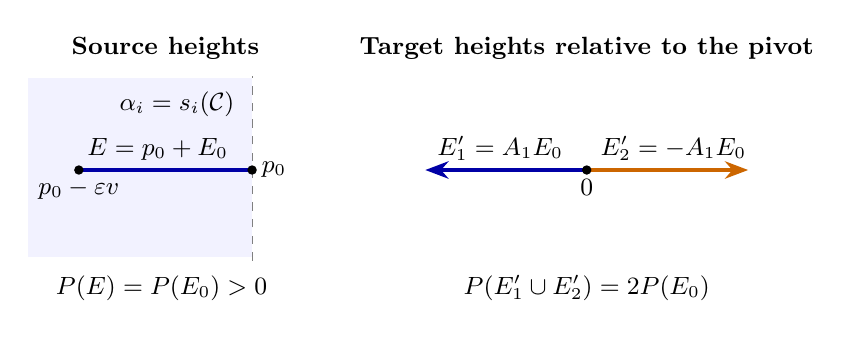
\begin{tikzpicture}[>=Stealth,font=\small]
 \begin{scope}
  \node[font=\small\bfseries] at (1.65,2.5) {Source heights};
  \fill[blue!5] (-.1,-.15) rectangle (2.75,2.12);
  \draw[gray,dashed] (2.75,-.2)--(2.75,2.15);
  \node[anchor=east] at (2.65,1.78) {$\alpha_i=s_i(\mathcal C)$};
  \draw[blue!65!black,very thick] (.55,.95)--(2.75,.95);
  \fill (.55,.95) circle (1.7pt);
  \fill (2.75,.95) circle (1.7pt);
  \node[below] at (.55,.95) {$p_0-\varepsilon v$};
  \node[right] at (2.75,.95) {$p_0$};
  \node[above] at (1.55,.95) {$E=p_0+E_0$};
  \node at (1.6,-.55) {$P(E)=P(E_0)>0$};
 \end{scope}
 \begin{scope}[xshift=7cm]
  \node[font=\small\bfseries] at (0,2.5) {Target heights relative to the pivot};
  \draw[blue!65!black,very thick,->] (0,.95)--(-2.05,.95);
  \draw[orange!80!black,very thick,->] (0,.95)--(2.05,.95);
  \fill (0,.95) circle (1.7pt);
  \node[below] at (0,.95) {$0$};
  \node[above] at (-1.1,.95) {$E'_1=A_1E_0$};
  \node[above] at (1.1,.95) {$E'_2=-A_1E_0$};
  \node at (0,-.55) {$P(E'_1\cup E'_2)=2P(E_0)$};
 \end{scope}
\end{tikzpicture}
\caption{The height geometry of the reflection contradiction. The two affine profiles agree at the facet pivot and send the inward segment to opposite target segments. Alternating bundles detect the volume exponent of their union. The picture is schematic: the exponential counts come from bracket-generated boxes, and the volume argument accounts for the nonuniqueness of lifts to $N\rtimes D$.}
\label{fig:reflection}
\end{figure}


\paragraph{Source bundles with a large joint volume.}
At a pivot $d_p\in D$ of height $rp_0$ and $D$-length $O(r)$, alternate
two sorts of bundles.  A first-sheet bundle updates the pair state by
$n\mapsto nu$.  A second-sheet bundle updates it by
$n\mapsto nkuk^{-1}$; on that sheet this is the generator movement
$nk\mapsto nku$.  Each bundle consists of a fixed finite sequence of
generator increments with widths $e^{rs_j(E)}$ and with independent
difference-of-interval parameters before restrictions are imposed.

We choose the source schemes and their number before restricting
parameters to good sheets.  Pass to a subsequence on which the normalized
bracket laws for $E$, $E'_1$, $E'_2$, and $E'_1\cup E'_2$ converge,
together with the bounded linear embeddings from either individual
target normalization into the union normalization.

The number of bundles is determined by multiplication in the target.
Consider the polynomial map multiplying alternating increments from
the two target boxes, with output normalized to $E'_1\cup E'_2$.
For a sufficiently large fixed number $h$ of increments, its limiting
map is submersive.  Indeed, every union-scaled generator attains its
support maximum in one of the two sets.  Its limiting vector therefore
belongs to the image of the corresponding limiting embedding.  These
vectors bracket-generate the union-normalized limiting algebra.
Finite products of exponentials from the two embedding images have
a submersive endpoint map: their conjugates span the generated Lie
algebra, and one inserts variable increments with those conjugates as
differentials.  Inserting identity factors makes the product alternating.
Fix such an $h$.  This rank property belongs to the full multiplication
map, before any target increments have been selected.

For each of the $h$ source bundles,
Lemma~\ref{lem:product-schemes} supplies an $E$-normalized generator
scheme with a submersive limiting product map.  Represent its scalar
parameters as independent differences of interval parameters.  The
schemes and their total number of switches are now fixed.  These
choices depend only on the normalized algebra data, not on $S_r$ or
the support tolerances.  Passing to this subsequence preserves the
profile approximations and the bound $\vol S_r/\vol Q_r\geq e^{-o(r)}$.
All the scaled $D$-legs lie in one compact subset over $\mathcal C$,
including their facet pivots.  The boundary convergence just established
therefore controls their profiles.

Apply backward recurrence to the individual switches in these bundles.
For a first-sheet switch with interval law $\sigma$, the increment law
is $\sigma*\check\sigma$.  For a second-sheet switch it is
$\sigma_k*\check\sigma_k$, where $\sigma_k=(\Ad_k)_*\sigma$ is the conjugated
interval law.
Thus all switches have the form required by
Lemma~\ref{lem:backward-recurrence}, with a depth independent of $r$.

Every recurrence denominator in Lemma~\ref{lem:backward-recurrence}
is at most $e^{o(r)}\vol Q_r$.  Indeed the supports in question are
products of a fixed number of $k_0^{\pm1}$, $k^{\pm1}$, and generator
intervals fitting the $\mathcal C$ widths, all with subexponential
factors.  The box calculus bounds the volume of the corresponding
support enlargements by $e^{o(r)}\vol B_r(\mathcal C)$.
Hence backward recurrence supplies a nonempty Borel subset of $S_r$
such that each initial state in that subset has conditional successful
parameter probability at least $e^{-o(r)}$, with every intermediate
pair state in $S_r$.  Fix one such state $n_0$.

Apply Corollary~\ref{cor:restricted-products} to the map from all bundle
parameters to the tuple of their products \emph{before} the conjugations
by $k$ and before accumulation.  The normalized map is the product of
$h$ submersive limiting polynomial maps.  The normalized pairs of
interval parameters have a fixed bounded joint density with respect
to Lebesgue measure.  Thus the successful probability just proved
gives successful Lebesgue measure at least $e^{-o(r)}$, even though
the restricted coordinates are correlated.  The image consequently
contains a compact set of $N^h$ Haar volume at least
$e^{rhP(E)-o(r)}$.  Conjugation by $k$ preserves Haar on $N$, and the
change from successive increments to successive states is triangular
and Haar preserving.  Consequently the admissible tuples
$(n_1,\ldots,n_h)$ of bundle-end states have the same lower volume.
This application takes place before conjugation, so it requires no
coefficient bound for a conjugation written in $E$-normalized
coordinates.

By Lemma~\ref{lem:fixed-sheet-packing}, the corresponding tuples
\[
 \bigl(F(xn_1d_p),\ldots,F(xn_hd_p)\bigr)
\]
have a separated-count lower bound $e^{rhP(E)-o(r)}$.
Take the source separation sufficiently large that the quasi-isometry
preserves a fixed target separation.  On the source side each terminal
point $xn_hd_p$ is reachable from $xn_0d_p$ by a path of length $O(r)$
whose relative heights lie in $r(E_0+o(1))$.  Use the $D$ legs over $E$
and return to the pivot after each generator switch.  Second-sheet
bundles use $o(r)$ bridges at the pivot.  Lemma~\ref{lem:path-packing}
therefore bounds the covering number of all source terminal points by
\begin{equation}\label{eq:source-reflection-count}
 e^{rP(E)+o(r)}
\end{equation}
at every fixed radius.

\paragraph{Target products have twice the terminal exponent.}
Put $y_j=F(xn_jd_p)$.  The successful profiles imply that the transition
from $y_{j-1}$ to $y_j$ has a path of length $O(r)$ with relative height
set $r(E'_{\tau(j)}+o(1))$, where $\tau(j)$ alternates between $1$ and
$2$.  All pivot height differences are $o(r)$, since the two limiting
affine profiles agree at $p_0$ and every intermediate state is good.
Choose lifts of these paths.  On accumulating them, the preceding
$D$ factors have height $o(r)$ and length $O(r)$; their conjugations
preserve the indicated box widths up to subexponential factors.
The endpoint lifts thus have the form
\[
 (u'_1\cdots u'_j,d'_j),\qquad
 u'_j\in B_r(E'_{\tau(j)},e^{o(r)}),\qquad
 |d'_j|_D=O(r),\quad \pi d'_j=o(r).
\]
Apply Lemma~\ref{lem:tuple-lift-volume} to the separated target tuples.
It gives a measurable increment set of Haar volume at least
$e^{rhP(E)-o(r)}$.  Dividing each factor by its box determinant shows
that this set has Lebesgue measure at least $e^{-o(r)}$ in the joint
individual-box log coordinates.  These coordinates lie in a cube of
radius $e^{o(r)}$.

Apply the alternating multiplication map used to choose $h$, with
output normalized to $E'_1\cup E'_2$.  Its degree is fixed, its
coefficients are bounded by the box calculus, and its limit is
submersive by that earlier choice.  These properties concern the full
map and therefore remain available for the measurable increment set
just obtained.

Lemma~\ref{lem:polynomial-image}, applied to the measurable increment
set, gives a compact set of terminal $N$ coordinates of volume at least
\[
 e^{rP(E'_1\cup E'_2)-o(r)}=e^{2rP(E)-o(r)}.
\]
Every such terminal coordinate has an accompanying $D$ coordinate of
length $O(r)$ and height $o(r)$ projecting near an image terminal.
The last assertion of Lemma~\ref{lem:tuple-lift-volume} bounds its
volume over any fixed-radius projected ball by $e^{o(r)}$.
But \eqref{eq:source-reflection-count} and the quasi-isometry cover all
image terminals by only $e^{rP(E)+o(r)}$ fixed-radius balls.  This is a
contradiction because $P(E)>0$.  The labels therefore agree for every
sufficiently small fixed $\delta$, as asserted.
\end{proof}

The preceding comparison leaves the offsets undetermined.  For fixed
$\delta$, a generator step can require a height exceeding the facet
by order $\delta r$; co-location alone would therefore leave an error
of order $\delta$ in the normalized affine offsets.  The next section
eliminates this error by a separate quotient-volume comparison.

\section{Comparing the offsets of neighboring sheets}
\label{sec:neighbor-offsets}

Proposition~\ref{prop:neighbor-labels} gives a common linear label for
neighboring sheet profiles.  It does not yet identify their constant terms.
At a fixed positive chart enlargement, the direct bridge between the sheets
can have length proportional to that enlargement times the scale.  We retain
this error and compare volumes in suitable nilpotent quotients.  Their Haar
multipliers will detect each component of the difference of the offsets.

\subsection{Quotients associated to cones of weights}

We first construct the quotients used in the comparison.  A word in the
generators $X_i$ is called \emph{pure for $S$} if every letter has weight in
$S$, and \emph{mixed for $S$} otherwise.  These terms will always refer to the
cone specified in the same argument.

\begin{lemma}[Cone quotients and their Haar multipliers]
\label{lem:cone-quotients}
Let $S\subset W^*$ be either the closed positive ray generated by a generator
weight $\alpha$, or the closed cone generated by two linearly independent
generator weights $\alpha,\lambda$.  The span $\mathfrak i_S$ of the mixed
words is a $\mathfrak d$-invariant ideal of $\mathfrak n$ containing
$\mathfrak d\cap\mathfrak n$.  Put
\[
 I_S=\exp_N(\mathfrak i_S),\qquad L_S=N/I_S.
\]
The group $I_S$ is closed, and $L_S$ is connected, simply connected, and
nilpotent.  Every compact subset of $L_S$ has compact lifts in $N$ and hence
in $G$.  There is a well-defined action of $G$ on $L_S$ under which $N$ acts
by left translations and $D$ acts by its induced conjugation automorphisms.  Write
\[
 p_S(g)=g\cdot 1_{L_S}.
\]
Then $p_S(gh)=g\cdot p_S(h)$ and the stabilizer of $1_{L_S}$ is $I_SD$.
There is a linear form $\ell_S\in W^*$ such that, for every Haar-measurable
$E\subset L_S$,
\begin{equation}
 \vol_{L_S}(g\cdot E)
   =e^{\ell_S(\pi g)}\vol_{L_S}(E).
 \label{eq:cone-haar-multiplier}
\end{equation}
The form $\ell_S$ is the sum of the weights of
$\mathfrak n/\mathfrak i_S$, counted with their dimensions.  It can be
expressed as a nonnegative integral combination of the inside generator
weights, with a positive coefficient for every inside generator.  In
particular, it is a positive multiple of $\alpha$ in the ray case, and it has
the form $c\alpha+d\lambda$, with $c,d>0$, in the two-generator case.
\end{lemma}

\begin{proof}
Bracketing a mixed word with any generator produces another mixed word.
The derivation identity and the Jacobi identity therefore show that their
span is the ideal generated by the outside letters.  Homogeneous bracket
words span $\mathfrak n$.  If a weight $\gamma$ lies outside $S$, a word of
weight $\gamma$ cannot be pure: a sum of inside weights belongs to $S$.
Consequently the entire generalized weight space
$\mathfrak n_\gamma$ lies in $\mathfrak i_S$ whenever $\gamma\notin S$.
For $v\in\mathfrak d$ and an outside letter $X_i$, the vector $[v,X_i]$
stays in $\mathfrak n_{\alpha_i}$ and hence in $\mathfrak i_S$.
Applying the derivation identity to words proves
$[\mathfrak d,\mathfrak i_S]\subset\mathfrak i_S$.  This argument includes
the nilpotent parts of the generalized weight actions.

Both possible cones $S$ are pointed.  A nonempty sum of their nonzero
inside weights cannot be zero.  The quotient algebra is spanned by pure
words, so it has no zero generalized weight space.  The zero weight space
of $\mathfrak n$ is therefore contained in $\mathfrak i_S$; in particular
$\mathfrak d\cap\mathfrak n\subset\mathfrak i_S$.
The exponential descriptions of the subgroups give $N\cap D\subset I_S$.
The ideal exponentiates to a closed subgroup because the exponential map
is a diffeomorphism and $\mathfrak i_S$ is a closed linear subspace.
The Baker--Campbell--Hausdorff group on $\mathfrak n/\mathfrak i_S$
identifies with $N/I_S$: the algebra quotient induces a surjective group
homomorphism with kernel $I_S$.  This realizes $L_S$ as a connected,
simply connected nilpotent Lie group.  A linear section of the algebra
quotient, composed with its logarithm and the exponential map of $N$,
gives a continuous section $L_S\to N$.  Images of compact sets under
this section are compact, proving the lifting assertion.

The action of $N\rtimes D$ on $L_S$ is
\[
 (n,d)\cdot(xI_S)=n(dxd^{-1})I_S.
\]
The kernel of the multiplication map $N\rtimes D\to G$ consists of
$(h^{-1},h)$ with $h\in N\cap D$.  Its action sends $xI_S$ to
$xh^{-1}I_S=xI_S$.  Thus the action factors through $G$, without requiring
that the multiplication map be injective.  If $g=nd$, its value at the
identity is $nI_S$, proving the stabilizer assertion and the stated
equivariance of $p_S$.

Translations by $N$ preserve quotient Haar measure.  The determinant of the
$D$-action is the exponential of its trace character; its unipotent parts
have determinant one.  The weight description thus gives
\eqref{eq:cone-haar-multiplier}.  To check its positivity assertion, project
to the abelianization of $\mathfrak n$.  The image of $\mathfrak i_S$ there
is exactly the span of the outside generator images.  The inside generator
images remain linearly independent in the quotient abelianization.  They
can be included in a basis of $\mathfrak n/\mathfrak i_S$ selected from pure
words.  Summing that basis's weights proves the asserted integral
combination.  Every inside weight in a two-generator cone is a nonnegative
real combination of its two defining weights, and each defining generator
itself survives.  Both extremal coefficients are therefore positive.
\end{proof}

For a ray we also use the notation $I_\alpha,L_\alpha,p_\alpha,\ell_\alpha$.
These objects depend on the oriented ray, rather than its representative.
For $A\in\mathcal A$ and a cone $S$, put
$S'=(A^*)^{-1}S$.  Lemma~\ref{lem:support-symmetries} ensures that $S'$ is a
cone of the same permitted kind, defined by the corresponding target
generator rays.

\subsection{Ideal boxes and a covering with controlled cardinality}

The quotient Haar multiplier will measure the difference between the two
offsets.  To make that comparison, we will cover the ideal coordinates by
translates of a smaller box and bound their number by the ratio of the
two box volumes.

Fix a cone $S$ as above and a Euclidean norm on $W$.  Write $I:=I_S$.
Define
\[
 T_* = \{v\in W:\|v\|\le1,\ \beta(v)\le0\text{ for every }\beta\in S\},
 \qquad T_j=\epsilon_jT_*,\quad j\in\{2,1,+\},
\]
where $0<\epsilon_2<\epsilon_1<\epsilon_+$.  An inside weight has support
maximum zero on $T_*$.  If $\beta\notin S$, separation from the closed
convex cone gives a vector nonpositive on $S$ and strictly positive on
$\beta$.  Rescaling that vector into the unit ball proves
$\max_{T_*}\beta>0$.  Hence
\begin{equation}
 \begin{aligned}
 h_Z(T_j)&=\epsilon_j c_Z,\qquad c_Z:=h_Z(T_*)>0
       &&\text{for every mixed word }Z,\\
 h_Z(T_j)&=0&&\text{for every pure word }Z.
 \end{aligned}
 \label{eq:cone-word-widths}
\end{equation}

Select a maximal-width basis of $\mathfrak i_S$ from mixed words and use it
to define the ideal box $B^I_r(T_j,L)$, by the same scaled-log-coordinate
construction as $B_r(T_j,L)$.  The same basis can be used for all three
$j$, since their widths differ by a positive scalar factor.  Complete it
to a basis of $\mathfrak n$ by pure words whose quotient images form a
basis.  This is a maximal-width basis of the whole algebra.  Indeed any
basis with too few mixed vectors can replace an excess pure vector by a
mixed vector, increasing its total width.  Once its mixed vectors form a
basis of $\mathfrak i_S$, their maximal possible total is the one selected
above, and the remaining widths are zero.  Thus, with $P_j=P(T_j)$,
\begin{equation}
 \vol_I B^I_r(T_j,L)\asymp L^{\dim I}e^{rP_j}
 \quad\text{for fixed }L>0.
 \label{eq:ideal-box-volume}
\end{equation}
The normalized multiplication and word-expansion bounds of
Lemma~\ref{lem:box-calculus} apply to these ideal boxes as well: brackets
of mixed words remain mixed, and their word widths add.

We will also use coordinates separating this ideal from its quotient.
Choose a linear section
$\sigma:\mathfrak n/\mathfrak i_S\to\mathfrak n$ whose image is spanned by
the selected pure words.  The map
\begin{equation}
 (i,z)\longmapsto i\exp_N\bigl(\sigma(\log_{L_S}z)\bigr)
 \label{eq:ideal-section-coordinates}
\end{equation}
is a bijection from $I_S\times L_S$ to $N$.  Projection determines $z$,
and then determines $i$.  Both this map and its inverse are polynomial in
log coordinates by the nilpotent product formula.  We verify explicitly
that product Haar measure in these coordinates is Haar measure on $N$,
up to a fixed scalar.  Write $s(z)=\exp_N(\sigma(\log_{L_S}z))$.
For $a\in N$, with quotient image $\bar a\in L_S$, left multiplication
acts on these coordinates by
\[
 a\,i\,s(z)=\bigl(\Ad_a(i)c_a(z)\bigr)s(\bar a z),
 \qquad c_a(z)=a s(z)s(\bar a z)^{-1}\in I.
\]
The inner automorphism $\Ad_a|_I$ has determinant one, since its
differential is the exponential of a nilpotent derivation.  The group
$I$ is unimodular, so right translation by $c_a(z)$ also preserves its
Haar measure.  Meanwhile $z\mapsto\bar a z$ preserves Haar measure on
$L_S$.  Fubini proves invariance of the pushed-forward product measure
under every left translation by $a$.  The coordinate diffeomorphism
makes this measure a nonzero Radon measure, so uniqueness of Haar
measure proves the assertion.
For a common sequential subexponential envelope, the box calculus gives
\begin{equation}
 n\in B_r(T_j,e^{o(r)})
 \quad\Longleftrightarrow\quad
 i\in B^I_r(T_j,e^{o(r)}),\quad
 \|\log_{L_S}z\|\le e^{o(r)},
 \label{eq:ideal-section-boxes}
\end{equation}
where the envelope may be enlarged on either side.  To see the forward
implication, use the adapted maximal basis: projection retains only its
zero-width pure coordinates.  Multiplying by the inverse section then
leaves an ideal element in the same enlarged box.  Conversely, the section
of a subexponential quotient log ball lies in the zero-width part of the
box, and multiplication gives the assertion.

\begin{lemma}[Strict-width covering and absorption]
\label{lem:strict-width-tiling}
Fix the cone, radii, and a letter $X_i$ with weight $\alpha\in S$.
Fix also $M>0$.  For all sufficiently small fixed $\delta>0$, the following
claims hold along every sequence $r\to\infty$.  Suppose
\[
 k_q=\exp(t_qX_i),\qquad |t_q|\le e^{M\delta r+o(r)}.
\]
There is a measurable partition of $B^I_r(T_1)$ into sets indexed by anchors
$i_\kappa\in B^I_r(T_1)$, with
\begin{align}
 \text{tile}_\kappa&\subset i_\kappa k_q B^I_r(T_2,O(1))k_q^{-1},
 &\#\{\kappa\}&\le e^{r(P_1-P_2)+o(r)},
 \label{eq:cone-tiles}\\
 k_q^{-1}i_\kappa k_q&\in B^I_r(T_+,O(1)).
 \label{eq:cone-anchor}
\end{align}
Moreover, if $u\in B_r(T_2,e^{o(r)})$ and $e_r\in N$ satisfies
$\|\log_N e_r\|\le e^{M\delta r+o(r)}$, the ideal coordinate of $ue_r$ in
\eqref{eq:ideal-section-coordinates} belongs to
$B^I_r(T_2,e^{o(r)})$.  These statements hold simultaneously for any fixed
finite collection of the cones, templates, and their images under
$\mathcal A$, after decreasing $\delta$.
\end{lemma}

\begin{proof}
If $Z$ is mixed, adjoining occurrences of $X_i$ does not change its width
on $T_*$, because $s_i(T_*)=0$.  In
\[
 \Ad_{k_q}Z
  =\sum_{p=0}^{m-1}\frac{t_q^p}{p!}(\ad X_i)^p Z,
\]
every nonzero term is mixed and has the same $c_Z$.  Its added exponential
cost is at most $pM\delta r+o(r)$.  Expanding a word in a maximal-width
ideal basis uses only basis vectors whose widths are at least its own,
by basis exchange.  Consequently the positive differences
\[
 (\epsilon_1-\epsilon_2)c_Z,
 \qquad (\epsilon_+-\epsilon_1)c_Z
\]
absorb all those costs if $\delta$ is sufficiently small.  There are only
finitely many words and $p<m$.  Their positive gaps also absorb the common
$o(r)$ envelope.  We obtain
\[
 k_qB^I_r(T_2,1)k_q^{-1}\subset B^I_r(T_1,O(1)),
 \qquad
 k_q^{-1}B^I_r(T_1,1)k_q\subset B^I_r(T_+,O(1)).
\]

Put $Q_r=k_qB^I_r(T_2,1)k_q^{-1}$.  Choose a maximal disjoint family
$i_\kappa Q_r$ with anchors in $B^I_r(T_1)$.  Such a family is finite: each set
lies in $B^I_r(T_1,O(1))$, by the first inclusion and normalized
multiplication.  Conjugation by $k_q$ preserves Haar on $I_S$, since its
derivative is the exponential of the nilpotent map
$\ad(t_qX_i)|_{\mathfrak i_S}$ and has determinant one.
Dividing volumes in \eqref{eq:ideal-box-volume} bounds the number of
anchors by $O(e^{r(P_1-P_2)})$.  Maximality implies that every translate
$iQ_r$, for $i\in B^I_r(T_1)$, meets some $i_\kappa Q_r$.  Hence
\[
 B^I_r(T_1)\subset\bigcup_\kappa i_\kappa Q_rQ_r^{-1}
  \subset\bigcup_\kappa i_\kappa k_qB^I_r(T_2,O(1))k_q^{-1}.
\]
Assign a point to the first set containing it.  This gives the measurable
partition, and the second inclusion above proves \eqref{eq:cone-anchor}.

For the last assertion write $u=i\exp_N\sigma(s)$, where
$i\in B^I_r(T_2,e^{o(r)})$ and $\|s\|\le e^{o(r)}$, using
\eqref{eq:ideal-section-boxes}.  Factor
\[
 \exp_N\sigma(s)e_r=i_{e_r}\exp_N\sigma(s_{e_r}).
\]
The polynomial coordinate maps show that
$\|\log i_{e_r}\|+\|s_{e_r}\|\le e^{M'\delta r+o(r)}$ for a fixed multiple
$M'$ of $M$.  Every ideal basis width on $T_2$ is strictly positive.
Decrease $\delta$ so that $M'\delta$ is less than all these widths.
Then $i_{e_r}\in B^I_r(T_2,O(1))$ for all sufficiently large $r$, and the ideal
coordinate $ii_{e_r}$ has the required bound.  Finitely many simultaneous
requirements have a positive common threshold for $\delta$.
\end{proof}

\subsection{Conditioned probes and the offset comparison}

We retain the profiles of Definition~\ref{def:chart-profiles}:
\[
 f_{r,x,n}(z)=\frac{\pi F(xn\Delta_rz)-\pi F(x)}r,
 \qquad a\text{ uniform in }B_r(\mathcal C),\quad n=ak_0,
\]
where $k_0\in B_r((1+\delta)\mathcal C,e^{o(r)})$ is independent of $a$.
All subexponential bounds below use one common vanishing envelope for the
finite constructions under consideration.  The maps and basepoints may
vary along the sequence.  We use
\[
 \mathcal U_\delta
  =\{z\in D_\infty:\pi z\in(1-c\delta)\operatorname{int}\mathcal C\}.
\]

\begin{proposition}[Equality of neighboring offsets]
\label{prop:neighbor-offsets}
There exists $\delta_2>0$ such that, for every fixed
$0<\delta\le\delta_2$, the following holds.  Let $r\to\infty$, let $F$ range
over the fixed family of smoothed quasi-isometries, let $x\in G$ vary, and
let $k_0$ be any allowed deterministic suffix.  For a generator letter
$X_i$, put
\[
 k=\exp(tX_i),\qquad |t|\le e^{(1+\delta)r s_i(\mathcal C)+o(r)}.
\]
Every pair in the support of any limiting joint law of
$(f_{r,x,ak_0},f_{r,x,ak_0k})$ has identical affine restrictions to
$\mathcal U_\delta$.  Equivalently, on every fixed compact subset of that
domain, the difference of these profiles tends to zero in probability.
The conclusion also holds for suffixes and steps sampled independently of
$a$, provided their bounds have a common vanishing envelope.
\end{proposition}

\begin{proof}
Take $\delta$ below the threshold in Proposition~\ref{prop:neighbor-labels}.
The two profiles in a limiting support then have the form
\[
 h_1(z)=A\pi z+b_1,\qquad h_2(z)=A\pi z+b_2
 \quad(z\in\mathcal U_\delta)
\]
with one $A\in\mathcal A$.  Fix such a pair and a subsequence whose joint
laws converge to a law containing it in its support.  It suffices to prove
$b_1=b_2$.  There are finitely many letters and labels, so these may be
fixed after passing to a subsequence.  Write $\alpha=\alpha_i$.

\paragraph{Choice of templates.}
We will use the ray cone of $\alpha$, and then each cone generated by
$\alpha$ and a generator weight independent of it.  Fix one of these
cones $S$, and put $S'=(A^*)^{-1}S$.  Let $p_0$ be the contact point of the
unit ball with the $\alpha$ facet of $\mathcal C$.  This point belongs to
the relative interior of that facet.  Choose a fixed $c'>c$ and put
\[
 w_q=(1-c'\delta)p_0.
\]
Choose fixed radii $0<\epsilon_2<\epsilon_1<\epsilon_+$ as above, small
enough that
\begin{equation}
 w_q+T_j\Subset(1-c\delta)\operatorname{int}\mathcal C
 \quad(j=2,1,+)
 \label{eq:offset-template-interior}
\end{equation}
for every sufficiently small fixed $\delta$.  Here $\Subset$ means compact
containment.  To verify the choice, the other oriented-ray facets have
positive slack at $p_0$; a sufficiently small fixed $\epsilon_+$ preserves
their inequalities.  On the $\alpha$ facet, $\alpha(T_j)\le0$, while
$c'>c$ gives a strict margin at $w_q$.  The radii can therefore be chosen
before $\delta$ tends to zero.  On the target templates $AT_j$ the inside
weights of $S'$ have width zero and all mixed words have positive width.
Also
\[
 P(AT_j)=P(T_j)=P_j.
\]

The comparison will balance three counts.  We will construct at least
$e^{rP_1-o(r)}$ separated source endpoints and assign them to at most
$e^{r(P_1-P_2)+o(r)}$ tiles.  For each tile we will prove an upper
bound
\[
 e^{r(P_2-\ell_{S'}(b_2-b_1))+o(r)}
\]
for the separated image endpoints.  The term $P_2$ comes from their
ideal coordinates; the remaining term is the Haar multiplier on the
quotient.  Summing over tiles cancels $P_2$ and will force
$\ell_{S'}(b_2-b_1)\le0$.  The construction below arranges these two
coordinate restrictions on the same endpoints.

Normalize the source at $w_q$ using the exact automorphism $S_{-rw_q}$, and
write $k_q=S_{-rw_q}k$.  Since $\alpha(p_0)=s_i(\mathcal C)$,
\[
 k_q=\exp(t_qX_i),\qquad
 |t_q|\le e^{(1+c')\delta r s_i(\mathcal C)+o(r)}.
\]
Use Lemma~\ref{lem:strict-width-tiling} to partition $B^I_r(T_1)$, with
anchors $i_\kappa$.  Choose a fixed unit cube $J$ in
$\mathfrak n/\mathfrak i_S$, and write $\sigma$ for the section used in
\eqref{eq:ideal-section-coordinates}.

\paragraph{Three paths chosen independently of the starting sheet.}
Sample $i_1$ uniformly in $B^I_r(T_1)$ and $s$ uniformly in $J$,
independently of the original random $a$.  Let $i_\kappa$ be the anchor assigned
to $i_1$, so the tile index $\kappa$ depends only on this probe.
For the moment $n=ak_0$ is still random.  Define
\begin{equation}
 n_1=nS_{rw_q}(i_1\exp_N\sigma(s)),\qquad
 n_{2,\kappa}=nS_{rw_q}(i_\kappa)k,\qquad
 n_2=nS_{rw_q}(i_1)k.
 \label{eq:offset-probes}
\end{equation}
We will count the endpoints $n_1$.  The auxiliary endpoint $n_2$
keeps the ideal probe $i_1$ and replaces the quotient factor by the
neighbor step $k$, while $n_{2,\kappa}$ gives one second-sheet anchor
for its tile.  Their design gives the exact cancellation
\begin{equation}
 n_1^{-1}n_2=S_{rw_q}\bigl(\exp_N(-\sigma(s))k_q\bigr).
 \label{eq:offset-probe-cancellation}
\end{equation}
This difference is independent of $i_1$.  A path from $n$ to $n_1$
will control the target quotient coordinate relative to the first
sheet.  A path from $n_{2,\kappa}$ to $n_2$, followed by the bridge
in \eqref{eq:offset-probe-cancellation}, will control the target ideal
coordinate of the same endpoint relative to its second-sheet anchor.

The following three sheet changes can be generated with uniformly bounded
numbers of generator switches:
\begin{align*}
 n&\longrightarrow n_1
       &&\text{using the template }w_q+T_1,\\
 nk&\longrightarrow n_{2,\kappa}
       &&\text{using the template }w_q+T_+,\\
 n_{2,\kappa}&\longrightarrow n_2
       &&\text{using the template }w_q+T_2.
\end{align*}
For the first, $i_1\exp_N\sigma(s)\in B_r(T_1,O(1))$ by
\eqref{eq:ideal-section-boxes}.  For the second, the relative normalized
increment is $k_q^{-1}i_\kappa k_q$, which satisfies
\eqref{eq:cone-anchor}.  For the third it is
$k_q^{-1}i_\kappa^{-1}i_1k_q\in B^I_r(T_2,O(1))$ by
\eqref{eq:cone-tiles}.  Lemma~\ref{lem:product-schemes}, followed by
$S_{rw_q}$, gives the stated generation with generator amplitudes at most
$e^{rs_j(w_q+T_l)+o(r)}$ for the indicated template $l$.

Choose these product representations measurably as functions of
$(i_1,s)$, using the measurable bounded product selection in
Lemma~\ref{lem:product-schemes}.  Its finite family of bounded schemes can
be padded by identity factors, and its Borel local inverse choices give
Borel parameters for every endpoint.  The anchors are already measurable.
All choices, including the product parameters and the paths below, are
independent of $a$.  The number of switches is bounded independently of
the probe parameters.  Every intermediate suffix is a fixed-length
product of the original allowed suffix and increments in the template
boxes, and, when needed, $k$.  The box calculus and
\eqref{eq:offset-template-interior} keep it in
$B_r((1+\delta)\mathcal C,e^{o(r)})$, with one envelope for all probes.

Choose a pivot $d_q\in D$ with $\pi d_q=rw_q$ and $|d_q|_D=O(r)$, for
example by exponentiating $r$ times a fixed linear lift of $w_q$ to
$\mathfrak d$.  Each generator switch can be performed by a $D$-leg from
the pivot to a support height of its template, the short switch there,
and a reversed $D$-leg on the new sheet.  The legs have length $O(r)$ and
the switches have length $o(r)$, by Lemmas~\ref{lem:log-distortion} and
\ref{lem:support-switch-paths}.  Their scaled $D$-coordinates lie in a fixed
compact subset of $\mathcal U_\delta$, by
Lemma~\ref{lem:d-scaling} and the strict containment
\eqref{eq:offset-template-interior}.  We fix a compact neighborhood of all
these coordinates for the remaining profile comparisons.

\paragraph{Why the intermediate profiles retain their starting offsets.}
This step uses only the affinity of individual limiting profiles.
Consider one of the selected generator switches, with template
$E\Subset(1-c\delta)\operatorname{int}\mathcal C$ and letter $X_j$.
There is a nonempty open set of heights in that domain on which
$\alpha_j(w)>s_j(E)$, because the support maximum is attained inside the
open domain.  On a smaller such open set the difference is bounded below
by a positive number.  At its $D$-positions, conjugating the switch back
gives exponentially decaying generator coefficients, up to polynomial
factors.  The distance of its two source sheet points, divided by $r$,
therefore tends to zero.  Their image profiles agree there in every
joint limit.  Proposition~\ref{prop:affine-profiles} makes each limiting
profile affine on $\mathcal U_\delta$, so equality on this open set gives
equality throughout that domain.

It follows by sequence compactness that the difference across each such
switch tends to zero in probability on the fixed compact set of legs.
This statement is uniform for the permitted parameter choices with their
common envelope: a violating sequence of choices would give a joint limit
contradicting the preceding open-set argument.  Conditioning on any
independent probe parameters and integrating proves the same assertion
for the measurable choices just made.  Since there are boundedly many
switches, with probability tending to one their intermediate profiles
all differ by $o(1)$ from the starting profile of their respective sheet.
The first path uses the profile of $n$; the other two use that of $nk$.

We now choose a single starting $n$ retaining a positive volume of probes.
For a fixed tolerance $\eta>0$, let $E_r(\eta)$ be the event that the
original pair of profiles is within $\eta$ of $(h_1,h_2)$ on the required
compact.  The support hypothesis gives
$\liminf_r\mathbb P(E_r(\eta))>0$.  Let $b_r(\eta)$ be the joint
probability, over the original chart sample and the independent probes,
that one of the intermediate profile comparisons has error exceeding
$\eta$.  The preceding paragraph gives $b_r(\eta)\to0$.
For large $r$ it is less than one quarter of
$\mathbb P(E_r(\eta))$.  Fubini's theorem then supplies an original sample
in $E_r(\eta)$ for which fewer than half of the probes fail these
comparisons.  First do this for each fixed tolerance and then let the
tolerance decrease sufficiently slowly with $r$.  We obtain a
deterministic starting $n=n_r$ and a measurable set of good probes of
probability at least $1/2$, on which all the required intermediate
profiles approach their designated affine maps.  This order of choices
does not condition on a null event, and it does not require every probe
to succeed simultaneously.

The generation selectors prescribe the paths; the probability law here
remains the original product of ideal Haar measure and Lebesgue measure
on $J$.  The preceding success events are measurable because the selected
parameters are Borel and the profiles depend continuously on their sheet
coordinates.  Inner regularity of this finite-dimensional product measure
allows us to retain a compact subset of good probes of probability at
least $1/4$.

The map $(i_1,s)\mapsto i_1\exp_N\sigma(s)$ is injective and carries
product Haar measure to Haar measure up to a fixed scalar.  The good
probe set thus has actual $N$-volume bounded below by a fixed positive
multiple of $e^{rP_1}$.  Since $S_{rw_q}$ has determinant one and left
translation by $n$ preserves Haar, the good values of $n_1$ in
\eqref{eq:offset-probes} have this same lower bound.  The possibly small
probability of the starting event has caused no loss of probe volume.
We use the compact retained subset from now on.  Its $n_1$-endpoint image
is compact, because $(i_1,s)\mapsto nS_{rw_q}(i_1\exp_N\sigma(s))$ is
continuous.  No continuity of the anchor assignment or generation
selectors is required; the tile partition is Borel and its anchor is
fixed on each tile.

\paragraph{The bridge and the two target restrictions.}
We now estimate the bridge in \eqref{eq:offset-probe-cancellation}.
At the pivot, conjugation by $d_q^{-1}$ cancels the character scaling
$S_{rw_q}$ and leaves only polynomially bounded unipotent factors.  As $s$
ranges in a fixed cube, the resulting logarithm has norm at most
$e^{C_1\delta r+o(r)}$.  Logarithmic distortion gives
\begin{equation}
 d_G(xn_1d_q,xn_2d_q)\le C_2\delta r+o(r),
 \label{eq:offset-bridge}
\end{equation}
where the constants are independent of sufficiently small fixed
$\delta$.  We retain this error at its stated size.

For good probes put
\[
 y_0=F(xnd_q),\quad y_1=F(xn_1d_q),\quad
 y_{2,\kappa}=F(xn_{2,\kappa}d_q),\quad y_2=F(xn_2d_q).
\]
The first probe path has target relative heights in
$r(AT_1+o(1))$, because its profiles approach $A\pi z+b_1$ and its pivot
height is $w_q$.  Its length is $O(r)$.  Path lifting and packing therefore
give a lift of $y_0^{-1}y_1$ with $N$-part in
$B_r(AT_1,e^{o(r)})$ and $D$-length $O(r)$.
Its endpoint height is $o(r)$, since both endpoint profiles approach
$Aw_q+b_1$.  Every pure quotient width is zero, so
\begin{equation}
 p_{S'}(y_0^{-1}y_1)\in \mathcal T_r,
 \qquad
 \mathcal T_r=\{z\in L_{S'}:\|\log z\|\le e^{o(r)}\},
 \qquad \vol_{L_{S'}}\mathcal T_r\le e^{o(r)}.
 \label{eq:offset-first-quotient}
\end{equation}
Choose its envelope large enough that the same restriction holds after
fixed bounded right thickening of the endpoints.  Indeed a bounded final
step keeps the first path's relative heights in $r(AT_1+o(1))$: its
unthickened endpoint height is $o(r)$ and $0\in AT_1$.  The same path
lifting estimate applies.

For a tile contributing a good probe, the second starting path and the
profile conditioning give
\begin{equation}
 \pi(y_0^{-1}y_{2,\kappa})=r(b_2-b_1)+o(r).
 \label{eq:offset-anchor-height}
\end{equation}
The path from $y_{2,\kappa}$ to $y_2$ has relative heights in
$r(AT_2+o(1))$, length $O(r)$, and endpoint height $o(r)$.
Choose its lift $u_2d_2$ with
\[
 u_2\in B_r(AT_2,e^{o(r)}),\qquad
 |d_2|_D=O(r),\qquad \pi d_2=o(r).
\]
A lift of the bridge from $y_2$ to $y_1$, using
\eqref{eq:offset-bridge} and the quasi-isometry bounds, has $N$ log norm
at most $e^{C_3\delta r+o(r)}$ and $D$-length $O(\delta r)+o(r)$.
Conjugating its $N$-part by $d_2$ changes this estimate only by a
subexponential factor.  We obtain a lift of $y_{2,\kappa}^{-1}y_1$ of the form
\begin{equation}
 u_2 e_r d,
 \qquad \|\log e_r\|\le e^{C_4\delta r+o(r)},\quad
 |d|_D=O(r),\quad \|\pi d\|\le O(\delta r)+o(r).
 \label{eq:offset-lift-with-error}
\end{equation}
The last height bound is only $O(\delta r)$, not $o(r)$.

Apply the absorption part of Lemma~\ref{lem:strict-width-tiling} to the
target ideal $I'=I_{S'}$ and template $AT_2$.  After decreasing $\delta$,
the ideal coordinate of $u_2e_r$ belongs to
$B^{I'}_r(AT_2,e^{o(r)})$.  More explicitly, factor
$u_2=i_2\exp\sigma'(s_2)$, with $\|s_2\|\le e^{o(r)}$.
Factoring $\exp\sigma'(s_2)e_r$ again produces an ideal error with log
norm $e^{O(\delta)r+o(r)}$.  Every mixed ideal width is strictly positive,
so this error fits in the ideal box.  This is an ideal-coordinate bound
uniform over the accompanying quotient coordinates; it does not require
their location to stay in a subexponential ball.

The bound remains valid under fixed bounded right thickening of the
lifts in \eqref{eq:offset-lift-with-error}.  Such thickening adds an
$N$-factor conjugated by $d$.  The stated $D$-length and
$O(\delta r)+o(r)$ height bounds make its logarithm at most
$e^{O(\delta)r+o(r)}$, and the same positive ideal widths absorb it.
This explicitly accounts for the non-sublinear height of the lift
relative to the second-sheet anchor.

All constants in the bridge and polynomial coordinate estimates can be
chosen independently of sufficiently small $\delta$: the radii are fixed,
the pivots stay in fixed compact height sets, and the quasi-isometry
constants are fixed.  There are finitely many cones, letters, and labels.
We choose $\delta_2$ small enough to satisfy all their strict gap and
absorption inequalities simultaneously.

The fixed-$\delta$ bridge has now been absorbed in the ideal-coordinate
bound.  It remains to compare quotient Haar volumes: their exact
multiplier will detect $\ell_{S'}(b_2-b_1)$.

\paragraph{Volume at an arbitrary translated quotient location.}
Fix a contributing tile and let $g_\kappa=y_{2,\kappa}^{-1}y_0$.  Equivariance in
Lemma~\ref{lem:cone-quotients}, together with
\eqref{eq:offset-first-quotient}, gives the exact restriction
\begin{equation}
 p_{S'}(y_{2,\kappa}^{-1}y_1)\in g_\kappa\cdot \mathcal T_r.
 \label{eq:offset-translated-quotient}
\end{equation}
It also holds for the thickened endpoints described above.  The Haar
multiplier and \eqref{eq:offset-anchor-height} imply
\begin{equation}
 \vol_{L_{S'}}(g_\kappa\cdot \mathcal T_r)
 \le e^{-r\ell_{S'}(b_2-b_1)+o(r)}.
 \label{eq:offset-quotient-volume}
\end{equation}
The set may be far from the quotient identity.  Its location has no
effect on this equality of Haar multipliers.

In the ideal and section coordinates \eqref{eq:ideal-section-coordinates},
every admissible $N$-part of the thickened lifts lies in a set with ideal
coordinate in $B^{I'}_r(AT_2,e^{o(r)})$ and quotient coordinate in
$g_\kappa\cdot \mathcal T_r$.  Quotient integration and
\eqref{eq:ideal-box-volume} bound its Haar volume by
\begin{equation}
 e^{r(P_2-\ell_{S'}(b_2-b_1))+o(r)}.
 \label{eq:offset-tile-N-volume}
\end{equation}
This is a bound by a containing product set.  It requires neither
independence of the coordinates nor a product description of the
admissible set, and holds at any translated quotient location.

To turn this into a separated-point bound, take image endpoints in this
tile with a fixed sufficiently large separation.  Choose the admissible
lifts relative to $y_{2,\kappa}$ and thicken each on the right by a fixed small
neighborhood in $N\rtimes D$.  Their projections lie in disjoint metric
balls, so these lifted neighborhoods are disjoint even if
$N\rtimes D\to G$ is not injective.  Each has the same positive product
Haar volume.  The thickened $D$-coordinates lie in an intrinsic $D$-ball
of radius $O(r)$, of polynomial volume.  The two coordinate restrictions
just proved still hold for all the neighborhoods.  Fubini's theorem and
\eqref{eq:offset-tile-N-volume} therefore bound their number by
\begin{equation}
 e^{r(P_2-\ell_{S'}(b_2-b_1))+o(r)}.
 \label{eq:offset-tile-count}
\end{equation}
The envelopes here are common to all contributing tiles, since the probe
paths, profile tolerances, and coordinate bounds were uniform over their
parameters.

The good $n_1$-volume was at least a constant times $e^{rP_1}$.
Lemma~\ref{lem:fixed-sheet-packing}, at the common pivot $d_q$, supplies
at least $e^{rP_1-o(r)}$ suitably separated source points from that set.
Take the separation large enough that their images are separated at the
constant used in \eqref{eq:offset-tile-count}.  Assign each chosen point
to its probe tile.  Summing \eqref{eq:offset-tile-count} over at most
$e^{r(P_1-P_2)+o(r)}$ tiles gives
\[
 e^{rP_1-o(r)}
 \le e^{r(P_1-\ell_{S'}(b_2-b_1))+o(r)}.
\]
Divide logarithms by $r$ and let $r\to\infty$.  We have proved
$\ell_{S'}(b_2-b_1)\le0$.

For the reverse inequality take the original starting suffix to be
$k_0k$ and the step to be $k^{-1}$.  The former is still in the allowed
enlarged box by normalized multiplication, with an enlarged common
subexponential envelope; the latter has the same generator amplitude
bound.  The swapped pair belongs to the swapped limiting support.
Repeating the argument gives $\ell_{S'}(b_1-b_2)\le0$.  Thus
\begin{equation}
 \ell_{S'}(b_2-b_1)=0
 \quad\text{for each of the specified cone tests.}
 \label{eq:offset-traces-vanish}
\end{equation}

\paragraph{The trace tests determine the offset.}
For the ray cone, its target trace is a positive multiple of
$\beta=(A^*)^{-1}\alpha$.  Hence $\beta(b_2-b_1)=0$.
For each generator weight $\lambda$ independent of $\alpha$, the target
two-generator trace is $c\beta+d\eta$, where
$\eta=(A^*)^{-1}\lambda$ and $c,d>0$.  Equation
\eqref{eq:offset-traces-vanish} then gives $\eta(b_2-b_1)=0$.
Weights proportional to $\alpha$ require no additional test.  Since the
generator weights span $W^*$, their target transforms do as well, proving
$b_2=b_1$.  When $\dim W=1$, the ray test alone gives this conclusion.

Finally, compactness converts the support assertion into convergence in
probability on each compact subset: any violation would admit a joint
limit assigning positive mass to unequal restrictions.  The same
contradiction works along arbitrary sequences of maps, basepoints, and
allowed deterministic choices with their fixed common envelope.
Conditioning on independently sampled suffixes and steps, or selecting
violating deterministic choices if convergence failed, gives the stated
random-choice version.
\end{proof}

\section{From random charts to uniform height control}
\label{sec:uniformity}

The preceding sections identify affine profiles and compare nearby
sheets.  We now remove the random chart center.  There are two distinct
points to check: the affine label must be independent of scale and
basepoint, and the chart offset must disappear after division by the
scale.  Throughout this section the Lipschitz, quasi-isometry and
coarse-inverse bounds for the pairs $(F,\bar F)$ are fixed.  All constants
are uniform over that family.

Choose $\delta>0$ small enough for Proposition~\ref{prop:neighbor-offsets},
and use $\mathcal C$, $\mathcal U_\delta$, and
$f_{r,x,n}$ from Definition~\ref{def:chart-profiles}.  Thus
\[
 f_{r,x,n}(z)=
 \frac{\pi F(xn\Delta_r z)-\pi F(x)}r,
 \qquad z\in D_\infty.
\]
Choose a compact identity neighborhood $Z\subset\mathcal U_\delta$.
In particular, $\pi Z$ contains a neighborhood of zero in $W$.
We can shrink $Z$ a fixed number of times below.

\begin{lemma}[Suffix comparison and concentration]
\label{lem:suffix-concentration}
Let $a$ be uniform on $B_r(\mathcal C)$.  Along every sequence
$r\to\infty$, with arbitrary maps $F$, basepoints $x$, and suffixes
\[
 k_0\in B_r((1+\delta)\mathcal C,e^{\eta_r r}),
 \qquad \eta_r\longrightarrow0,
\]
one has
\begin{equation}
\label{eq:suffix-profile-comparison}
 \|f_{r,x,ak_0}-f_{r,x,a}\|_Z\longrightarrow0
 \quad\text{in probability}.
\end{equation}
The assertion also holds for suffixes sampled independently of $a$
whose supports satisfy the same bound.

There are deterministic $A_{F,x,r}\in\mathcal A$ and $s_{F,x,r}\in W$
such that
\begin{equation}
\label{eq:ordinary-chart-concentration}
 \sup_{F,x}\mathbb E\left\|
 f_{r,x,a}-A_{F,x,r}\pi-\frac{s_{F,x,r}}r
 \right\|_Z\longrightarrow0,
 \qquad |s_{F,x,r}|\le C r.
\end{equation}
The same approximation holds in probability with $a$ replaced by
$ak_0$ in the sequential setting of
\eqref{eq:suffix-profile-comparison}.
\end{lemma}

\begin{proof}
By Lemma~\ref{lem:product-schemes}, an allowed suffix is a product
of a bounded number of generator exponentials.  Their amplitudes obey
the bounds of Proposition~\ref{prop:neighbor-offsets}; all partial
products remain allowed suffixes by Lemma~\ref{lem:box-calculus}.
The joint law of each successive pair of profiles is relatively
compact by Proposition~\ref{prop:affine-profiles}.  Every limit is
supported on identical pairs by Proposition~\ref{prop:neighbor-offsets}.
The distance between the two profiles on $Z$ therefore tends to zero
in probability.  Summing over the bounded number of steps proves
\eqref{eq:suffix-profile-comparison}.  If independent random suffixes
violated the assertion, conditioning would select deterministic
suffixes with failure probability bounded below.  This would contradict
the deterministic statement.

Write $\mu_r$ for uniform Haar probability on $B_r(\mathcal C)$.
The normalized product bounds give a fixed $L\ge1$ such that
\[
 a^{-1}B_r(\mathcal C)\subset B_r(\mathcal C,L)
 \qquad(a\in B_r(\mathcal C)).
\]
Let $k$ be independent and uniform on $B_r(\mathcal C,L)$.
For each fixed $a$, the conditional law of $ak$ dominates $c\mu_r$
for a constant $c>0$ independent of $r$ and $a$.  Indeed, its Haar
density on $aB_r(\mathcal C,L)$ is the reciprocal of the volume of
that box, and the ratio of this volume to $\vol B_r(\mathcal C)$
is bounded.  Consequently, for independent $a,b$ with law $\mu_r$,
\[
 \Pr\{\|f_{r,x,a}-f_{r,x,b}\|_Z>\epsilon\}
 \le c^{-1}
 \Pr\{\|f_{r,x,a}-f_{r,x,ak}\|_Z>\epsilon\}
 \longrightarrow0.
\]

The ordinary profile laws are relatively compact and uniformly bounded
on $Z$.  If $\nu$ is any subsequential limit, the last display says that
$\nu\times\nu$ is supported on the diagonal.  Thus $\nu$ is a point
mass.  Proposition~\ref{prop:affine-profiles} says that this point has
the form $A\pi+b$, with $A\in\mathcal A$.

Set
\[
 s_{F,x,r}=r\,\mathbb E f_{r,x,a}(1),
\]
and choose $A_{F,x,r}\in\mathcal A$ to minimize the expected supremum
norm in \eqref{eq:ordinary-chart-concentration}.  These quantities
are well defined because the profiles are bounded.  The point-mass
conclusion proves convergence to zero along every sequence of maps
and basepoints; otherwise a violating sequence would have a
point-mass subsequential limit for which the minimum is zero.
This proves the stated supremum over $F,x$.
Finally $|a|_G\le Cr$ by Lemma~\ref{lem:log-distortion}, so the
Lipschitz bound for $F$ gives $|s_{F,x,r}|\le Cr$.
Equation~\eqref{eq:suffix-profile-comparison} transfers the deterministic
approximation to the allowed suffixes.
\end{proof}

\begin{remark}
\label{rem:suffix-envelope}
The suffix assertion is sequential.  Equivalently, one can prescribe
a vanishing envelope $\eta(r)$ for any fixed finite collection of
constructions and then take the corresponding uniform bounds.  It
does not mean a supremum at a fixed $r$ over every sequence that might
eventually satisfy $\eta_r\to0$.  The supremum in
\eqref{eq:ordinary-chart-concentration} concerns ordinary charts and
has no such suffix parameter.
\end{remark}

\begin{lemma}[Stabilization across scales]
\label{lem:scale-stabilization}
There is $R_0$ independent of $F,x$ such that $A_{F,x,r}$ is independent
of $r\ge R_0$.  Moreover
\[
 \sup_{F,x}|s_{F,x,r}|/r\longrightarrow0.
\]
\end{lemma}

\begin{proof}
Put $q=1+\delta/2$.  If $r\le r'\le qr$, let $a$ be uniform on
$B_r(\mathcal C)$ and let $k$ be independent and uniform on
$B_{r'}(\mathcal C,L)$, for a sufficiently large fixed $L$.
For every such $a$,
\[
 a^{-1}B_{r'}(\mathcal C)\subset B_{r'}(\mathcal C,L).
\]
The density argument in Lemma~\ref{lem:suffix-concentration} shows
that the law of $ak$ dominates a fixed multiple of uniform measure
on $B_{r'}(\mathcal C)$.  This suffix fits the strict expansion at
scale $r$, since $r'\le(1+\delta/2)r$.

For the same $N$-coordinate $n$, compare the two deterministic
approximations at
\[
 z'=\Delta_{r'}^{-1}\Delta_rz,
 \qquad r'\pi z'=r\pi z.
\]
On a fixed smaller $Z$, $z'$ stays in the original neighborhood.
The errors of both approximations are $o(r)$ in probability,
uniformly over $r'\in[r,qr]$, $F$, and $x$.  To justify this last
uniformity, a violating sequence would be an allowed sequence in
Lemma~\ref{lem:suffix-concentration}, with the fixed envelope coming
from $L$; the density comparison constants are fixed.
More precisely, the lower domination of the law of $ak$ transfers
its scale-$r$ good event to uniform measure on $B_{r'}(\mathcal C)$.
Intersect there with the ordinary scale-$r'$ good event.
Therefore
\begin{equation}
\label{eq:scale-affine-comparison}
 \sup_{z\in Z}
 \left|s_{F,x,r}-s_{F,x,r'}
       +r(A_{F,x,r}-A_{F,x,r'})\pi z\right|=o(r).
\end{equation}
The expression is deterministic: an event of positive probability
on which both approximations are accurate proves its bound.

Subtract \eqref{eq:scale-affine-comparison} at $1$ from its values
at a fixed finite set of points whose heights span $W$.
The offsets cancel.  Distinct members of the finite set $\mathcal A$
are separated on these heights, so the labels agree for all
$r\ge R_0$, with one $R_0$.  Since any larger scale can be reached
by successive ratios in $[1,q]$, the label stabilizes.
Evaluating at $1$ also gives
\[
 |s_{F,x,r'}-s_{F,x,r}|\le\varepsilon(r)r
 \quad(r\le r'\le qr),\qquad \varepsilon(r)\longrightarrow0,
\]
uniformly in the other variables.

For completeness, fix $\epsilon>0$ and choose a fixed $R\ge R_0$
such that $\varepsilon(t)\le\epsilon$ for $t\ge R$.
Telescope along scales $R,qR,q^2R,\ldots$, ending with a ratio
at most $q$.  The uniform bound at the initial scale gives
\[
 |s_{F,x,r}|
 \le CR+\epsilon\sum_{j:q^jR<r}q^jR
 \le CR+\frac{q}{q-1}\epsilon r.
\]
First divide by $r$ and let $r\to\infty$, then let $\epsilon\to0$.
This proves the uniform sublinear bound.
\end{proof}

\begin{proposition}[Uniform sublinear height estimate]
\label{prop:uniform-sublinear}
For each map $F$ there is a single $A_F\in\mathcal A$ and there is
a function $\epsilon(R)\to0$, common to the entire fixed family,
such that
\begin{equation}
\label{eq:uniform-sublinear}
 \left|\pi F(xg)-\pi F(x)-A_F\pi g\right|
 \le\epsilon(R)R
 \qquad(F,\ x\in G,\ |g|_G\le R).
\end{equation}
The label of the coarse inverse is $A_{\bar F}=A_F^{-1}$.
\end{proposition}

\begin{proof}
It remains to compare the stabilized labels and center values at
different basepoints.  Fix a sufficiently small $\eta>0$ relative
to $\delta$.  Suppose $|x^{-1}y|_G\le\eta r$ and choose a lift
\[
 x^{-1}y=ud,\qquad
 |d|_D\le C(1+\eta r),\qquad
 \|\log u\|\le e^{C(1+\eta r)}
\]
using Lemma~\ref{lem:path-packing}.  Set $r_0=(1-\delta/2)r$ and,
for $a$ uniform on $B_r(\mathcal C)$, put
\[
 a_y=d^{-1}u^{-1}ad.
\]
Its law has constant Haar density $1/\vol B_r(\mathcal C)$ on
its support, since conjugation by $d$ has determinant one.

Let $a_0$ be uniform on $B_{r_0}(\mathcal C)$ and let $k$ be
independent and uniform on
$d^{-1}B_r(\mathcal C,L)d$.  We claim that the law of $a_y$
is dominated by a fixed multiple of the law of $a_0k$.
Indeed, for every possible $a,a_0$,
\[
 \Ad_d(a_0^{-1}a_y)=(\Ad_da_0)^{-1}u^{-1}a
 \in B_r(\mathcal C,L).
\]
The inclusion follows from Lemma~\ref{lem:box-calculus}:
the smaller box retains a strict exponent gap after conjugation
by $d$, and $u$ fits strictly within the $r$-widths if $\eta$
is small enough.  Polynomial conjugation factors are absorbed by
these gaps.  The Haar volume of the box for $k$ is a fixed
multiple of $\vol B_r(\mathcal C)$.  Conditional density comparison,
followed by integration in $a_0$, proves the claim.

All these $k$ lie in the allowed expansion at scale $r_0$.
For this use
$(1+\delta)(1-\delta/2)>1$ and choose $\eta$ smaller if necessary;
the remaining strict gap again absorbs the polynomial factors.
Thus Lemma~\ref{lem:suffix-concentration} applies with a common
envelope to this collection of comparisons.

We have the exact identity
\[
 xa\Delta_rz=ya_y d^{-1}\Delta_rz.
\]
For $z$ in a fixed smaller neighborhood, the point
$z'=\Delta_{r_0}^{-1}(d^{-1}\Delta_rz)$ lies in $Z$.
This follows from Lemma~\ref{lem:d-scaling} and the small bound
on $|d|_D/r$; its height satisfies exactly
\[
 r_0\pi z'=r\pi z-\pi d.
\]
The two deterministic chart approximations, transferred through
the fixed density domination, can now be compared.  Their offsets
are $o(r)$ by Lemma~\ref{lem:scale-stabilization}.  Subtracting the
comparison at two values of $z$ cancels both center values and
$\pi d$.  Testing a fixed spanning set of heights forces equality
of the stabilized labels at $x,y$, uniformly for all sufficiently
large $r$.  Evaluation at $z=1$ then gives
\[
 \pi F(y)-\pi F(x)-A_{F,y,r_0}\pi(x^{-1}y)=o(r),
 \qquad |x^{-1}y|_G\le\eta r,
\]
uniformly in $F,x,y$.

Any two basepoints can be compared at a sufficiently large scale;
therefore the stabilized label is a single $A_F$.
To obtain \eqref{eq:uniform-sublinear} for $|g|\le R$, take
$y=xg$ and $r=R/\eta$.  The preceding uniform error then provides
one modulus $\epsilon(R)\to0$ for all maps and basepoints.

Finally apply \eqref{eq:uniform-sublinear} to both maps in a
coarse-inverse pair.  For $g_t=\exp_D(tH)$, the displacement
$F(g_t)$ from $F(1)$ is $O(t)$.  Bounded-error composition gives
\[
 t\pi H
 =A_{\bar F}A_F(t\pi H)+o(t).
\]
Every $w\in W$ is $\pi H$ for some $H\in\mathfrak d$.
Division by $t$ proves $A_{\bar F}A_F=\id$.
\end{proof}

\section{Quotient boundaries and bounded height error}
\label{sec:boundary}

We now strengthen Proposition~\ref{prop:uniform-sublinear} to a bounded
error.  A ray quotient records the directions that contract when one
height tends to minus infinity.  The sublinear estimate produces
homeomorphisms of these quotients.  Comparing the volumes of their
images first bounds height variation along $N$-fibers.  Averaging the
image volumes of translates in the source quotient then controls the
remaining $D$-directions.

Boundary actions play a central role in \cite[Theorem~2 and Section~4]{Dymarz2010} and
\cite[Section~4.1]{DymarzFisherXie2025}.  Here the contracting quotient
boundaries are used to compare Haar volumes of boundary images and
bound the height error.

\subsection{Contracting rays and boundary homeomorphisms}

For a generator ray represented by a nonzero form $\alpha$, abbreviate
the objects of Lemma~\ref{lem:cone-quotients} by
\[
 I_\alpha=I_{\R_{\ge0}\alpha},\qquad
 L_\alpha=N/I_\alpha,\qquad p_\alpha(g)=g\cdot1,\qquad
 \ell_\alpha=\ell_{\R_{\ge0}\alpha}.
\]
Multiplying $\alpha$ by a positive scalar does not change these
objects.  Every weight of $\Lie(L_\alpha)$ is a strictly positive
multiple of $\alpha$, and
\begin{equation}
\label{eq:ray-trace}
 \ell_\alpha=c_\alpha\alpha,\qquad c_\alpha>0.
\end{equation}
The positivity follows because at least one generator class on this
ray survives in the quotient abelianization.
Fix one representative of each target generator ray, and use its
pullbacks by the finitely many members of $\mathcal A$ when a source
representative is needed.  We fix left invariant Riemannian metrics
on the finitely many ray quotients.

We use two elementary consequences of the quotient action.
If $y=nd$ is any lift of an element of $G$, then
\begin{equation}
\label{eq:quotient-step}
 p_\beta(yh)=p_\beta(y)\,
     \Ad_d\bigl(p_\beta(h)\bigr).
\end{equation}
Here $\Ad_d$ denotes the induced automorphism on $L_\beta$.
The formula is independent of the lift because $N\cap D\subset I_\beta$.
Also, for each fixed compact set $Q\subset L_\beta$, there are
$C,M,c>0$ such that
\begin{equation}
\label{eq:quotient-contraction}
 \sup_{q\in Q}\|\log(\Ad_d q)\|
 \le C(1+|d|_D)^M e^{c\beta(\pi d)}
 \qquad\text{if }\beta(\pi d)\le0.
\end{equation}
Indeed the quotient has finitely many weights $c_j\beta$, $c_j>0$;
take $c=\min_jc_j$ and use the polynomial bounds on their unipotent
parts from Lemma~\ref{lem:canonical-height},
Equation~\eqref{eq:d-polynomial-unipotent}.  These statements also hold
for compact families of bounded increments.

\begin{lemma}[Boundary maps from sublinear height control]
\label{lem:ray-boundaries}
Let $F$ belong to the fixed Lipschitz quasi-isometry family, let
$A=A_F$, and let $\beta$ be a selected target ray representative.  Put
$\alpha=\beta\circ A$.  There is a homeomorphism
\[
 f_\beta:L_\alpha\longrightarrow L_\beta
\]
and a fixed compact set $Q_\beta\subset L_\beta$ such that
\begin{equation}
\label{eq:boundary-shadow}
 f_\beta(p_\alpha x)\in F(x)\cdot Q_\beta
 \qquad(x\in G).
\end{equation}
The compact sets may be chosen uniformly over the fixed family.
The map obtained from $\bar F$ for the reversed ray pair is
$f_\beta^{-1}$.
\end{lemma}

\begin{proof}
Since $\mathcal A^*$ permutes the generator rays, the source quotient
is defined.  Choose $v\in\mathfrak d$ with $\alpha(\pi v)<0$.
There are only finitely many ray and label choices, so choose all
these $v$'s once.

\smallskip
\noindent\emph{Convergence and a uniform compact shadow.}
For $x_t=x\exp_D(tv)$, Proposition~\ref{prop:uniform-sublinear} gives
\[
 \beta\bigl(\pi F(x_t)-\pi F(x)\bigr)
 =t\alpha(\pi v)+o(t)\le-c_0t
 \qquad(t\ge T_0),
\]
with $c_0,T_0>0$ uniform in $F,x$ and the finite choices.
Set $y_t=F(x)^{-1}F(x_t)$.  Its distance from $1$ is $O(1+t)$.
By Lemma~\ref{lem:path-packing} it has a lift $y_t=n_td_t$ with
$|d_t|_D\le C(1+t)$.  The increments $y_t^{-1}y_{t+1}$ have
uniformly bounded length and hence bounded lifts.  Equations
\eqref{eq:quotient-step} and \eqref{eq:quotient-contraction} imply
\[
 \left\|\log\bigl(p_\beta(y_t)^{-1}p_\beta(y_{t+1})\bigr)\right\|
 \le C(1+t)^M e^{-c_1t}.
\]
The series is summable.  In a left invariant Riemannian metric,
$d(1,\exp Z)\le C\|Z\|$, by using the path $s\mapsto\exp(sZ)$.
Thus the projected trajectory at integer times is Cauchy and stays
in a fixed closed ball.  Completeness and properness of the metric
give convergence in a fixed compact set.
The same estimate for time increments of size at most one gives
convergence for real $t\to\infty$.  The initial interval
$0\le t\le T_0$ contributes a fixed compact set, so the limit lies
in a fixed compact $Q_\beta$.  Equivariance of $p_\beta$ under
the $G$-action therefore gives a limit
\begin{equation}
\label{eq:boundary-limit}
 b(x)=\lim_{t\to\infty}p_\beta F(x\exp_D(tv))
 \in F(x)\cdot Q_\beta .
\end{equation}

\smallskip
\noindent\emph{Independence of the representative.}
We first record the path estimate used for this purpose.
Suppose, for large $t$, a source path stays at distance at most
$C_2t$ from a fixed $x$, has length bounded by a polynomial in $t$,
and satisfies
\[
 \alpha\bigl(\pi(x^{-1}z)\bigr)\le-c_2t
\]
at each of its points $z$.  The uniform sublinear estimate puts
its image, relative to $F(x)$, at $\beta$-heights at most
$-c_2t/2$ for all sufficiently large $t$.
The lifts at all image points have $D$-length $O(t)$, because
their distance from $F(x)$ is $O(t)$.
Subdivide the source path into bounded-length pieces.
Equations~\eqref{eq:quotient-step} and
\eqref{eq:quotient-contraction} bound each projected image increment
by a polynomial times $e^{-ct}$.  There are only polynomially many
pieces, so the projected distance between the endpoints tends to
zero.  Constants here may depend on this fixed collection of paths.

For fixed $d\in D$, connect $x\exp(tv)$ to $xd\exp(tv)$ by
$xd(s)\exp(tv)$, where $d(s)$ is a fixed piecewise smooth path in
$D$ from $1$ to $d$.  Its length is polynomial in $t$, since
conjugation in the nilpotent group $D$ has polynomial norm.
Its points have distance $O(t)$ from $x$, and their relative
$\alpha$-heights equal $t\alpha(\pi v)+O(1)$.
The preceding path estimate gives $b(xd)=b(x)$.

For fixed $u\in I_\alpha$, we will vary the height within the halfspace
$\alpha<0$ to realize $u$ while keeping the $\alpha$-height strongly negative.
Choose a compact convex set $E\subset W$ containing $\pi v$,
entirely in $\alpha<0$, such that every bracket
word containing an outside-ray letter has $h_Z(E)>0$.
Here is why such an $E$ exists.  Every generator form outside the
positive $\alpha$-ray is unbounded above on the halfspace
$\{\alpha\le\alpha(\pi v)\}$.  For each outside form choose a point
in that halfspace on which it is as large as desired, and take
the convex hull together with $\pi v$.  The support maxima for
inside-ray letters remain fixed negative numbers.  Since the
list of words and their lengths is finite, sufficiently large
outside maxima make the support sum of every mixed word positive.

By Lemma~\ref{lem:cone-quotients}, the mixed words span
$\Lie(I_\alpha)$.  Thus the fixed element $u$ belongs to
$B_t(E,O(1))$ for all sufficiently large $t$.
One can see this directly in the all-word description of the box:
the fixed coordinates of $\log u$ in a mixed-word basis are
dominated by its positive exponential widths.
Choose an affine section $\sigma:W\to V$ of $\pi$ with
$\sigma(\pi v)$ equal to the abelianization of $v$.
The compact convex set $E_V=\sigma(E)$ contains that
abelianization and satisfies $\pi E_V=E$.
The paths of Lemma~\ref{lem:support-switch-paths}, applied to $E_V$
and the pivot $\exp(tv)$, connect $\exp(tv)$ to $u\exp(tv)$ in length
$O(t)$ with heights in $t(E+o(1))$.  All their heights remain
strictly negative in $\alpha$ by a linear amount, and all their
points have distance $O(t)$ from $1$.  Left translation by $x$
and the preceding path estimate give $b(xu)=b(x)$.

The stabilizer of $1\in L_\alpha$ is $I_\alpha D$.
The two invariances therefore show that $b(x)$ depends only on
$p_\alpha x$.  Define $f_\beta(p_\alpha x)=b(x)$.
This establishes \eqref{eq:boundary-shadow}.

\smallskip
\noindent\emph{Inverse and continuity.}
By Proposition~\ref{prop:uniform-sublinear},
$A_{\bar F}=A^{-1}$, so the construction for $\bar F$ gives
$\bar f:L_\beta\to L_\alpha$.
For $x_t=x\exp(tv)$ the quotient point $p_\alpha x_t$ is fixed.
Equation~\eqref{eq:boundary-shadow} at $x_t$ supplies representatives
$z_t$ of $f_\beta(p_\alpha x)$ within a fixed distance of $F(x_t)$:
lift the compact set $Q_\beta$ to a bounded set in $G$.
The coarse-inverse estimate and the shadow estimate for $\bar f$
then give
\[
 \bar f(f_\beta(p_\alpha x))\in x_t\cdot Q'
\]
for a fixed compact $Q'\subset L_\alpha$.
The sets on the right contract to $p_\alpha x$, since
$\alpha(\pi v)<0$.  Thus $\bar f f_\beta=\id$.
Interchanging the maps proves $f_\beta\bar f=\id$.

Fix $x$ and $t$.  The projection of a fixed-radius neighborhood
of $x_t$ contains a neighborhood of $p_\alpha x$; this uses only
that the quotient projection is a submersion.
By the Lipschitz bound and \eqref{eq:boundary-shadow}, its image
under $f_\beta$ is contained in $F(x_t)\cdot Q''$, with $Q''$
fixed.  These sets have diameter tending to zero.
Indeed, after normalization by $F(x)$, the $D$-part has length
$O(t)$ and negative linear $\beta$-height, so
\eqref{eq:quotient-contraction} applies; quotient left translations
are isometries.  The fixed action of $F(x)$ is Lipschitz, being
a left translation followed by an automorphism.
This proves continuity at $p_\alpha x$.  The same argument proves
continuity of $\bar f$, completing the proof.
\end{proof}

\subsection{Boundary volumes and variation along \texorpdfstring{$N$}{N}-fibers}

\begin{lemma}[Volumes of boundary images]
\label{lem:boundary-volume}
For each source and target ray pair in Lemma~\ref{lem:ray-boundaries},
there is a fixed compact ball $U\subset L_\alpha$ with nonempty
interior such that
\begin{equation}
\label{eq:boundary-volume}
 \vol_{L_\beta}\bigl(f_\beta(x\cdot U)\bigr)
 \asymp e^{\ell_\beta(\pi F(x))}
 \qquad(x\in G).
\end{equation}
The comparison constants and the choices of balls are uniform
over the fixed quasi-isometry family.
\end{lemma}

\begin{proof}
Fix a unit ball $V_-\subset L_\beta$ and a bounded set of lifts
of radius $R_-$ in $G$.  Denote the common Lipschitz constants
by $L_F,L_{\bar F}$ and the common coarse-inverse error by $E_0$.
For each such lift $b$,
\[
 d_G(\bar F(F(x)b),x)\le L_{\bar F}R_-+E_0.
\]
The shadow estimate for the inverse boundary map therefore puts
$f_\beta^{-1}(F(x)\cdot V_-)$ inside $x\cdot U$, where $U$ is
one compact ball containing
\[
 \{h\cdot q:|h|_G\le L_{\bar F}R_-+E_0,\ q\in Q_{\rm inv}\}.
\]
Here $Q_{\rm inv}$ is its fixed shadow compact.
This choice of $U$ is independent of $x$.

Choose a bounded lift set for this $U$ once, of radius $R_U$.
For every lift $b$ in it,
$d_G(F(xb),F(x))\le L_FR_U$.
The forward shadow estimate gives
$f_\beta(x\cdot U)\subset F(x)\cdot V_+$ for one compact $V_+$.
Thus
\[
 F(x)\cdot V_-\subset f_\beta(x\cdot U)
 \subset F(x)\cdot V_+.
\]
Both comparison sets have positive finite Haar volume.
The $G$-action scales that volume by
$e^{\ell_\beta(\pi F(x))}$, proving the assertion.
There are finitely many ray and label choices, so all constants
can be chosen uniformly.
\end{proof}

\begin{lemma}[Bounded variation on \(N\)-fibers]
\label{lem:leaf-height}
There is a uniform constant $B_N$ such that
\[
 |\pi F(xn)-\pi F(x)|\le B_N
 \qquad(F,\ x\in G,\ n\in N).
\]
In particular $|\pi F(nd)-\pi F(d)|\le B_N$ for all $n\in N,d\in D$.
\end{lemma}

\begin{proof}
Fix a generator $X_i$ and any $t\in\R$.
For every source generator ray other than that of $\alpha_i$,
the element $\exp(tX_i)$ lies in its ideal and acts trivially
on the corresponding quotient.  Hence the two source sets
\[
 x\exp(tX_i)\cdot U,\qquad x\cdot U
\]
are identical.  Lemma~\ref{lem:boundary-volume} bounds the difference
of the associated target trace heights by a uniform constant.
By \eqref{eq:ray-trace}, this bounds every target ray-height
difference except possibly the ray paired with $\alpha_i$.

There is a relation $\sum_\rho c_\rho\rho=0$ over all distinct
target generator rays, with every $c_\rho>0$, by
Lemma~\ref{lem:support-symmetries}.  Applying it to the height
difference bounds the one remaining form as well.
Since the ray forms span $W^*$, there is a uniform constant
$B_1$ with
\[
 |\pi F(x\exp(tX_i))-\pi F(x)|\le B_1
\]
for every $x,i,t$.  No bound on $t$ is imposed.

The sets $B_r(\mathcal C)$ exhaust $N$, since every generator
support maximum on $\mathcal C$ is positive.  By
Lemma~\ref{lem:product-schemes}, every such box element is a
product of at most one fixed number $M$ of generator exponentials.
Their parameters can be arbitrary, because the preceding estimate
is parameter independent.  Thus $B_N=MB_1$ works for every $n$.
Finally $nd=d(d^{-1}nd)$ and $d^{-1}nd\in N$; applying the bound
at the basepoint $d$ proves the last assertion without introducing
any dependence on $d$.
\end{proof}

\subsection{Averaging and bounded height}

Fix a ray pair, its boundary map $f_\beta$, and the ball $U$ from
Lemma~\ref{lem:boundary-volume}.  Pull target Haar measure back to
$L_\alpha$ by this map.  For $d\in D$, the preceding two lemmas make
the mass of every left translate of $d\cdot U$ comparable to
$e^{\ell_\beta(\pi F(d))}$, independently of the translating element.
The next lemma compares this common mass with the source Haar volume
of $d\cdot U$.  Since that volume scales by
$e^{\ell_\alpha(\pi d)}$, the comparison will relate source and target
height characters.

\begin{lemma}[Averaging translates of a Radon measure]
\label{lem:haar-averaging}
Let $L$ be a connected simply connected nilpotent Lie group with
Haar measure $\mu$ and a left invariant Riemannian metric.
Let $\rho$ be a Radon measure on $L$.
Suppose a family of compact positive-Haar-measure sets $E_j$,
including $E_0$, and positive numbers $a_j$ satisfy
\[
 K^{-1}a_j\le\rho(zE_j)\le Ka_j
 \qquad(z\in L,\ j)
\]
for one $K\ge1$.  Then
\[
 \frac{a_j}{\mu(E_j)}\asymp
 \frac{a_0}{\mu(E_0)}
\]
with constants depending only on $K$ and a large-scale volume
doubling constant of $L$, independently of the shapes and diameters
of the sets.  Absolute continuity of $\rho$ is not required.
\end{lemma}

\begin{proof}
For compact $E\subset B(R_E)$ and $T>R_E$, Tonelli's theorem gives
\[
 \int_{B(T)}\rho(zE)\,d\mu(z)
 =\int_L\mu(B(T)\cap yE^{-1})\,d\rho(y).
\]
Nilpotent groups are unimodular, so inversion preserves Haar
measure.  The inner quantity equals $\mu(E)$ for
$y\in B(T-R_E)$, vanishes outside $B(T+R_E)$, and lies between
zero and $\mu(E)$ everywhere.  Consequently
\begin{equation}
\label{eq:haar-kernel-bounds}
 \mu(E)\rho(B(T-R_E))
 \le \int_{B(T)}\rho(zE)\,d\mu(z)
 \le \mu(E)\rho(B(T+R_E)).
\end{equation}

Fix a large-scale doubling constant $D_0$ such that
$\mu(B(2T))\le D_0\mu(B(T))$ for all sufficiently large $T$.
Such a constant follows from the polynomial volume estimates for
nilpotent groups, as in Lemma~\ref{lem:d-scaling}.
Put $q_0=a_0/\mu(E_0)$.
Apply \eqref{eq:haar-kernel-bounds} to $E_0$, first with averaging
radius $T-R_{E_0}$ and then with radius $T+R_{E_0}$.
The assumed translate bounds and doubling give, for sufficiently
large $T$,
\[
 (KD_0)^{-1}q_0\mu(B(T))
 \le\rho(B(T))\le KD_0q_0\mu(B(T)).
\]
For a fixed $j$, choose $T$ so large that these bounds apply to
$T-R_{E_j}$ and $T+R_{E_j}$ and that $T\ge2R_{E_j}$.
Use \eqref{eq:haar-kernel-bounds} for $E_j$ and the assumed
translate bounds once more.  Doubling yields
\[
 (K^2D_0^2)^{-1}q_0
 \le\frac{a_j}{\mu(E_j)}
 \le K^2D_0^2q_0.
\]
The required averaging radius may depend on $j$; the displayed
constants do not.  Only integration of nonnegative measurable
functions was used, so the proof applies equally to singular
Radon measures.
\end{proof}

\begin{proof}[Proof of Theorem~\ref{thm:bounded-height}]
If $W=0$, the assertion is immediate.  Otherwise first take a
Lipschitz pair from the uniform family of
Lemma~\ref{lem:lipschitz-pairs}, with label $A_F$ from
Proposition~\ref{prop:uniform-sublinear}.
Fix a target ray $\beta$ and its source ray
$\alpha=\beta\circ A_F$.  Let $f_\beta$ and $U$ be given by
Lemmas~\ref{lem:ray-boundaries} and \ref{lem:boundary-volume}.
Define a Radon measure on $L_\alpha$ by
\[
 \rho(E)=\vol_{L_\beta}(f_\beta(E)).
\]
This is a measure because $f_\beta$ is a homeomorphism; no
absolute-continuity property is asserted.

For $d\in D$, put $U_d=d\cdot U$ and
$a_d=e^{\ell_\beta(\pi F(d))}$.
Every $z\in L_\alpha$ has a representative $n\in N$, and
$zU_d=nd\cdot U$.
Lemmas~\ref{lem:boundary-volume} and \ref{lem:leaf-height} give
\[
 \rho(zU_d)\asymp a_d
 \qquad(z\in L_\alpha,d\in D)
\]
with one uniform comparison constant.
Lemma~\ref{lem:haar-averaging}, applied to these sets and the
reference set $U_1=U$, implies
\[
 \frac{e^{\ell_\beta(\pi F(d))}}{\vol_{L_\alpha}(U_d)}
 \asymp
 \frac{e^{\ell_\beta(\pi F(1))}}{\vol_{L_\alpha}(U)}.
\]
The source action scales Haar by $e^{\ell_\alpha(\pi d)}$.
Taking logarithms therefore gives
\begin{equation}
\label{eq:trace-height-bound}
 \ell_\beta(\pi F(d)-\pi F(1))
 =\ell_\alpha(\pi d)+O(1)
 \qquad(d\in D),
\end{equation}
with a uniform error.

We identify its linear term using the already proved sublinear
estimate.  For $w\in W$, choose $H\in\mathfrak d$ with $\pi H=w$
and set $d_t=\exp_D(tH)$.  Its length is $O(t)$, so
\eqref{eq:trace-height-bound} and
Proposition~\ref{prop:uniform-sublinear} give
\[
 t\ell_\alpha(w)+O(1)
 =\ell_\beta(\pi F(d_t)-\pi F(1))
 =t\ell_\beta(A_Fw)+o(t).
\]
After division by $t$,
$\ell_\alpha=\ell_\beta\circ A_F$.
The target ray traces span $W^*$ by \eqref{eq:ray-trace}.
A fixed spanning subfamily of \eqref{eq:trace-height-bound}
therefore yields
\[
 |\pi F(d)-\pi F(1)-A_F\pi d|\le B_D
 \qquad(d\in D),
\]
with uniform $B_D$.
For any $g=nd$, Lemma~\ref{lem:leaf-height} and $\pi n=0$
extend this bound to $g$, with bound $B_D+B_N$.
All finite ray and label choices were absorbed into the constants,
so the conclusion holds for the whole fixed family.

Finally an original $(K,C)$ quasi-isometry is at a uniformly
bounded distance from its Lipschitz approximation by
Lemma~\ref{lem:lipschitz-pairs}.  Since $\pi$ is Lipschitz,
changing back alters the error by a uniform constant, proving
the stated theorem for the original maps.
\end{proof}

\section{From bounded heights to polycyclicity}
\label{sec:recognition}

We now apply Theorem~\ref{thm:bounded-height} to an arbitrary finitely
generated group quasi-isometric to a virtually polycyclic group.  The
geometric step produces a homomorphism whose kernel is locally virtually
nilpotent, meaning that every finitely generated subgroup of the kernel is
virtually nilpotent.  This proves elementary amenability.  Finiteness and
duality theorems then supply a polycyclic subgroup of finite index.

\subsection{The two Lie models}

Two Lie groups serve different purposes below.  A solvable Lie group $S$
contains a finite-index subgroup of the comparison group as a uniform
lattice; its compact quotient supplies finiteness and Poincar\'e duality.
A real-triangulable group $G$, quasi-isometric to $S$, supplies the height
geometry.  We do not require a lattice in $G$.

For the lattice model, we use the following finiteness terminology.
A group $L$ is of type $F$ if it has a finite CW classifying space.
It is of type $\FP_n(\Z)$ if the trivial module $\Z$ has a projective resolution over $\Z L$ that is
finitely generated through degree $n$, and of type $\FP_\infty(\Z)$ if
this holds in every degree.  Its integral cohomological dimension
$\operatorname{cd}_{\Z}L$ is the minimum length of a projective
$\Z L$-resolution of $\Z$, or infinity if no finite-length resolution
exists.  Type $F$ implies both $\FP_\infty(\Z)$ and finite integral
cohomological dimension.  The recognition argument will use these two
consequences separately.

We use the algebraic characterization of an integral Poincar\'e duality
group of dimension $n$: the trivial module $\Z$ admits a finite-length
resolution by finitely generated projective $\Z L$-modules, and
\[
 H^i(L;\Z L)=0\quad(i\ne n),
 \qquad H^n(L;\Z L)\cong\Z\quad\text{as abelian groups}.
\]
The right $L$-module $H^n(L;\Z L)$ is the orientation module; its action
may be nontrivial, so orientability is not part of our convention.
See \cite[Theorem~9.2 and Section~9.10]{Bieri1981} and the discussion preceding
\cite[Corollary~4.48]{Li2018}.

\begin{lemma}\label{lem:model-reduction}
Let $P$ be a finitely generated virtually polycyclic group, and let $H$ be
a finitely generated group quasi-isometric to $P$.  There exist a
finite-index subgroup $\Gamma\leq P$, a connected simply connected
solvable Lie group $S$, and a connected simply connected real-triangulable
unimodular Lie group $G$ such that
\[
 \Gamma\text{ is a uniform lattice in }S,
 \qquad H\simeq_{\mathrm{QI}}P\simeq_{\mathrm{QI}}S
             \simeq_{\mathrm{QI}}G.
\]
The group $H$ is amenable.  Moreover, $\Gamma$ has a finite classifying
space and is an integral Poincar\'e duality group of dimension $\dim S$.
\end{lemma}

\begin{proof}
Dekimpe's lattice realization theorem
\cite[Theorem~4.1]{Dekimpe2000} gives $\Gamma$ and $S$, with $\Gamma$
normal of finite index in $P$ if desired.  The uniform lattice acts
properly and cocompactly by left translations on $S$.  Thus its inclusion
is a quasi-isometry by the Milnor--\v{S}varc lemma; the same observation
applies to a finite-index subgroup acting on a Cayley graph.  See
\cite[Theorem~4.C.5(1) and Proposition~4.C.11(3)]{CornulierDeLaHarpe2016}.
Cornulier--Tessera's reduction
\cite[Lemma~3.A.1]{CornulierTessera2017} gives a real-triangulable $G$
quasi-isometric to $S$.  It remains to check unimodularity and the stated
properties of $H$ and $\Gamma$.

The group $P$ is amenable, since cyclic groups are amenable and this
property is preserved by extensions and finite extensions.  We give the
metric F\o lner argument that transfers this information to $G$ and $H$.
It is important here to obtain metric F\o lner sets in $G$, rather than
only amenability as a locally compact group; compare
\cite[Proposition~11.11 and Corollary~11.13]{Tessera2008}.

Let $Y$ denote either $G$, with a left invariant Riemannian metric and
left Haar measure $\mu$, or $H$, with a word metric and counting measure.
Choose a quasi-isometry $u:P\to Y$ with coarse-surjectivity radius $c>0$,
and fix $a>c$.  For finite nonempty $E\subset P$, put
\[
 A_E=\bigcup_{p\in E} B_Y(u(p),a).
\]
For each fixed radius, the lower quasi-isometry inequality bounds the
number of points of $P$ whose images lie in a ball of that radius.
Consequently the balls in this union have bounded multiplicity, and
\begin{equation}\label{eq:recognition-folner-lower}
 \mu(A_E)\geq c_1|E|
\end{equation}
for a constant $c_1>0$ independent of $E$.

Write $N_R(A)$ for the metric $R$-neighborhood of a set $A$.  If
$y\in N_R(A_E)\setminus A_E$, choose $p_y\in P$ with
$d_Y(y,u(p_y))\leq c$ and $p\in E$ with
$d_Y(y,u(p))\leq R+a+1$.  Since $a>c$, we have $p_y\notin E$.
The lower quasi-isometry inequality gives
$d_P(p_y,E)\leq R'$, with $R'$ depending only on $R,a$ and the
quasi-isometry constants.  It follows that
\begin{equation}\label{eq:recognition-folner-boundary}
 \mu\bigl(N_R(A_E)\setminus A_E\bigr)
 \leq \mu(B_Y(1,c))\,|N_{R'}(E)\setminus E|.
\end{equation}
An increasing-radius F\o lner sequence in $P$, together with
\eqref{eq:recognition-folner-lower}--\eqref{eq:recognition-folner-boundary},
therefore gives finite-measure sets $A_j\subset Y$ satisfying
\begin{equation}\label{eq:recognition-metric-folner}
 \frac{\mu(N_R(A_j))}{\mu(A_j)}\longrightarrow1
 \qquad\text{for every fixed }R.
\end{equation}
For the discrete group $H$, this is the F\o lner criterion for
amenability.

For $Y=G$, right translation by $g$ moves every point a distance
$d_G(1,g)$, so $A_jg\subset N_{d_G(1,g)}(A_j)$.  If right translation
multiplied left Haar measure by a factor greater than one, this inclusion
would contradict \eqref{eq:recognition-metric-folner}.  A nontrivial
modular homomorphism has such a value, after replacing $g$ by $g^{-1}$
if necessary.  Thus $G$ is unimodular.

Finally, a connected simply connected solvable Lie group of dimension
$n$ is diffeomorphic to $\R^n$; explicit coordinates are given in
\cite[Lemma~3.B.2]{CornulierTessera2017}.
The compact smooth manifold $\Gamma\backslash S$ is therefore
aspherical and has a finite CW structure.  It is a finite classifying
space for $\Gamma$, and manifold Poincar\'e duality makes $\Gamma$ an
integral Poincar\'e duality group of dimension $n$.
\end{proof}

\subsection{Polynomial growth in a height kernel}

The polynomial packing estimate needed here is stronger than an estimate
of the form $e^{o(t)}$.  Lemma~\ref{lem:polynomial-path-packing} gives
that estimate for paths whose heights remain bounded at every point.
We record carefully how it applies to a subgroup with its own word
metric.

\begin{lemma}\label{lem:height-kernel-growth}
Let $G$ be a connected simply connected real-triangulable unimodular Lie group with the height
homomorphism $\pi:G\to W$, and let $f:H\to G$ be a quasi-isometry from
a finitely generated group, normalized by $f(e)=1$.  Suppose $H_0\leq H$
and $\tau:H_0\to W$ is a homomorphism such that, for some $D<\infty$,
\begin{equation}\label{eq:recognition-corrected-height}
 \|\pi f(h)-\tau(h)\|\leq D\qquad(h\in H_0).
\end{equation}
Then every finitely generated subgroup of $K_0=\ker\tau$ has polynomial
growth and is virtually nilpotent.
\end{lemma}

\begin{proof}
Fix a finitely generated subgroup $J\leq K_0$ and a finite symmetric
generating set $T$ of $J$.  The heights of all orbit points $f(j)$,
$j\in J$, have norm at most $D$.  For a word
$j=t_1\cdots t_m$ with $m\leq t$, put
$j_i=t_1\cdots t_i$.  The upper quasi-isometry inequality gives a
constant $L_T$ such that
\[
 d_G(f(j_{i-1}),f(j_i))\leq L_T
 \qquad(1\leq i\leq m).
\]
Join these successive points by minimizing geodesics.  The resulting
path starts at $1$, ends at $f(j)$, and has length at most $L_Tt$.
The homomorphism $\pi$ is Lipschitz for a left invariant Riemannian
metric: its differential has constant norm in left-trivialized tangent
spaces.  If $L_\pi$ is a Lipschitz constant, every point of the path has
height norm at most $D+L_\pi L_T$.

Lemma~\ref{lem:polynomial-path-packing}, with these fixed length and
height bounds, shows that a maximal $1$-separated subset of
$f(B_T(t))$ has at most $C_T(1+t)^{b_T}$ points.  The unit balls about
that subset cover $f(B_T(t))$.  The lower quasi-isometry inequality
bounds the number of elements of $H$ mapping into each such ball by
one constant: any two such elements are at uniformly bounded distance
in the fixed word metric of $H$.  Hence
\[
 |B_T(t)|\leq C'_T(1+t)^{b_T}.
\]
This is an intrinsic growth bound for $J$; no undistortion of $J$ in $H$
is assumed.  Gromov's polynomial-growth theorem
\cite[Main Theorem, p.~54]{Gromov1981} makes $J$ virtually nilpotent.
\end{proof}

The packing input works with lifts to $N\rtimes D$:
compactly bounded increment lifts place chosen endpoint lifts in a
polynomial-volume coordinate region.  Separation in $G$ separates
these lifts, as in Lemma~\ref{lem:polynomial-path-packing}, so the
argument applies even when $N\cap D\ne\{1\}$.

\subsection{The transferred action and elementary amenability}

We use the term \emph{elementary amenable} for the smallest class of
groups containing finite and abelian groups and closed under subgroups,
quotients, extensions, and directed unions.  In the next proposition
amenability is a hypothesis, but elementary amenability is a conclusion.

\begin{proposition}\label{prop:recognition-from-height}
Let $G$ be a connected simply connected real-triangulable unimodular Lie
group with height homomorphism $\pi:G\to W$.  Let $H$ be a finitely
generated amenable group quasi-isometric to $G$.  Assume the uniform
bounded-height conclusion of Theorem~\ref{thm:bounded-height} for the
family of self-quasi-isometries transferred from left translations of
$H$.  Then there is a finite-index normal subgroup $H_0\leq H$ and a
homomorphism $\tau:H_0\to W$ whose kernel is locally virtually
nilpotent.  In particular, $H$ is elementary amenable.
\end{proposition}

\begin{proof}
Choose quasi-inverse maps $f:H\to G$ and $r:G\to H$.  Bounded changes
allow us to arrange $f(e)=1$ and $r(1)=e$.  For $h\in H$, define
\[
 F_h=f\circ L_h\circ r,
 \qquad L_h(k)=hk.
\]
The maps $F_h$ have uniform quasi-isometry constants, because the maps
$L_h$ are isometries.  There is a constant $D_0$ such that
\begin{equation}\label{eq:recognition-quasiaction}
 \sup_{g\in G}d_G(F_hF_k(g),F_{hk}(g))\leq D_0
 \qquad(h,k\in H),
\end{equation}
and $F_e$ is uniformly close to the identity.  These assertions follow
from the bounded errors in $r\circ f$ and $f\circ r$.  Also
$F_h(1)=f(h)$.

Put $s(h)=\pi f(h)$.  The assumed height theorem gives a single
$B<\infty$ and matrices $A_h$ in the fixed finite group $\A_G$
such that
\begin{equation}\label{eq:recognition-affine-action}
 \|\pi F_h(g)-s(h)-A_h\pi(g)\|\leq B
 \qquad(h\in H,\ g\in G).
\end{equation}
Apply this formula twice to $F_hF_k(g)$, and compare with its application
to $F_{hk}(g)$ using \eqref{eq:recognition-quasiaction}.  It follows
that
\[
 (A_hA_k-A_{hk})\pi(g)
\]
is bounded as $g$ ranges over $G$.  Since $\pi$ is surjective onto the
vector space $W$, its linear coefficient vanishes.  Similarly $A_e=I$.
Thus $h\mapsto A_h$ is a homomorphism, and
\[
 H_0=\{h\in H:A_h=I\}
\]
is normal and has finite index.  Evaluating the same comparison at
$g=1$ gives a constant $D_1$ such that
\begin{equation}\label{eq:recognition-defect}
 \|s(hk)-s(h)-s(k)\|\leq D_1\qquad(h,k\in H_0).
\end{equation}
The uniform constant in the height theorem is essential here: $D_1$
does not depend on $h$ or $k$.

The subgroup $H_0$ is amenable.  Let $m$ be a left-invariant mean on
bounded real functions on $H_0$, extended coordinatewise to functions
with values in $W$.  Define
\begin{equation}\label{eq:recognition-mean}
 \tau(h)=m_x\bigl(s(hx)-s(x)\bigr),\qquad h\in H_0.
\end{equation}
For fixed $h$, the function being averaged is bounded, since
\eqref{eq:recognition-defect} bounds its distance from $s(h)$ by $D_1$.
Positivity of the mean gives
\begin{equation}\label{eq:recognition-mean-error}
 \|\tau(h)-s(h)\|\leq D_1.
\end{equation}
To verify additivity, write
\[
 s(hkx)-s(x)=s(hkx)-s(kx)+s(kx)-s(x).
\]
Left invariance under $x\mapsto kx$ shows that the means of the two
terms on the right are $\tau(h)$ and $\tau(k)$.  Therefore
$\tau(hk)=\tau(h)+\tau(k)$.

Let $K_0=\ker\tau$.  Equation~\eqref{eq:recognition-mean-error} is
the hypothesis of Lemma~\ref{lem:height-kernel-growth}; that lemma
makes each finitely generated subgroup of $K_0$ virtually nilpotent.
Nilpotent groups are elementary amenable by their central series, and
so are their finite extensions.  The finitely generated subgroups of
$K_0$ form a directed family with union $K_0$.  Thus $K_0$ is elementary
amenable.  The exact sequence
\[
 1\longrightarrow K_0\longrightarrow H_0
   \overset{\tau}{\longrightarrow}\tau(H_0)\longrightarrow1
\]
and abelianness of $\tau(H_0)$ show that $H_0$ is elementary amenable.
Finally $H/H_0$ is finite, so $H$ is elementary amenable as well.
\end{proof}

The image $\tau(H_0)$ need not be discrete in $W$, and the kernel $K_0$
need not be finitely generated.  Neither property was used: abelianness
of the image and the directed-union argument are sufficient.

\subsection{Finiteness, duality, and the conclusion}

The previous proposition supplies elementary amenability.  To complete
recognition, we first transfer $\FP_\infty(\Z)$ from the comparison
lattice.  The elementary amenable finiteness theorem then gives a
finite-index subgroup of type $F$, which supplies the finite
cohomological dimension needed for duality transfer.

\begin{proof}[Proof of Theorem~\ref{thm:recognition}]
Let $P$ and $H$ satisfy the hypotheses of the theorem.  Apply
Lemma~\ref{lem:model-reduction} and retain both the real-triangulable
unimodular model $G$ and the uniform lattice $\Gamma\leq S$.

If $W=0$, Lemma~\ref{lem:canonical-height} makes $G$ nilpotent.  Its metric
balls have polynomial Haar volume, by the nilpotent coordinate bounds
of Lemma~\ref{lem:d-scaling}.  A quasi-isometry from $H$ to $G$ has
bounded multiplicity on bounded scales, so disjoint small-ball packing
transfers this to polynomial word growth of $H$.  Gromov's theorem
\cite[Main Theorem, p.~54]{Gromov1981} makes $H$ virtually nilpotent,
hence virtually polycyclic.  This also includes the zero-dimensional
model: in that case $H$ is finite.  We may therefore suppose $W\ne0$.

By Lemma~\ref{lem:model-reduction}, $H$ is amenable.  Apply
Theorem~\ref{thm:bounded-height} to the uniform family transferred
from its left translations.  Proposition~\ref{prop:recognition-from-height}
shows that $H$ is elementary amenable.

The group $\Gamma$ has a finite classifying space and is quasi-isometric
to $H$.  Li's coarse invariance theorem
\cite[Corollary~4.47]{Li2018}, applied over $\Z$ for each $n$, gives
$H\in\FP_\infty(\Z)$.  The elementary amenable finiteness theorem
\cite[Theorem~1.1, (viii)$\Rightarrow$(v)]{KrophollerMartinezPerezNucinkis2009}
now gives a finite-index subgroup $V\leq H$ of type $F$.  The structural
conclusion recorded in Section~2 of the same paper also gives a
finite-index solvable subgroup $U\leq H$.  Set $H_1=U\cap V$.
Then $H_1$ is solvable and has finite index in $H$.  The finite cover of
a finite classifying space for $V$ corresponding to $H_1$ is a finite
classifying space for $H_1$.  In particular,
\[
 \operatorname{cd}_{\Z}H_1<\infty.
\]
This also implies that $H_1$ is torsion-free: restriction of a finite
projective resolution to a hypothetical nontrivial finite cyclic
subgroup would give finite integral cohomological dimension for that
subgroup, which is impossible.

Both $H_1$ and $\Gamma$ now have finite integral cohomological dimension,
and they are quasi-isometric.  Since $\Gamma$ is an integral
Poincar\'e duality group, Li's duality transfer
\cite[Corollary~4.48]{Li2018}, with coefficient ring $\Z$, makes $H_1$
an integral Poincar\'e duality group.  Here the type-$F$ subgroup supplies
the finite-cohomological-dimension hypothesis.  Bieri's theorem
\cite[Theorem~9.23]{Bieri1981} says that a solvable integral
Poincar\'e duality group is polycyclic.  Hence $H_1$ is polycyclic, and
$H$ is virtually polycyclic.
\end{proof}

\begin{proof}[Proof of Corollary~\ref{cor:lattice-recognition}]
Let $\Lambda$ be a lattice in a connected simply connected solvable Lie
group $S$.  Such a lattice is polycyclic
\cite[Proposition~3.4]{FarbWeinberger2008}, and is uniform
\cite[Theorem~2.9(i)]{Geng2015}.  It is therefore finitely generated and
quasi-isometric to $S$ by the Milnor--\v{S}varc lemma.  A finitely
generated group $H$ quasi-isometric to $\Lambda$, or equivalently to
$S$, is virtually polycyclic by Theorem~\ref{thm:recognition}.
Dekimpe's realization theorem \cite[Theorem~4.1]{Dekimpe2000} then
embeds a finite-index subgroup of $H$ as a uniform lattice in some
connected simply connected solvable Lie group.

Conversely, every virtually polycyclic comparison group has such a
finite-index lattice model by the same realization theorem.  Finite
index preserves quasi-isometry, so the lattice formulation implies the
group formulation.  The ambient Lie group obtained for $H$ is not
prescribed by this equivalence.
\end{proof}

\appendix
\section{Lipschitz representatives}
\label{app:lipschitz-representatives}

We prove the uniform replacement lemma used to construct the compact
space of quasi-isometry pairs in Section~\ref{sec:stationary}.

\begin{proof}[Proof of Lemma~\ref{lem:lipschitz-pairs}]
A coarse inverse can first be chosen with constants depending only on
$K,C$.  Indeed, for each target point choose a source point whose image
is within the coarse-surjectivity constant.  The two quasi-isometry
inequalities bound the distortion of this choice and its two composition
errors.  It is therefore enough to smooth either member of a uniformly
controlled coarse-inverse pair by a bounded amount.

Choose a maximal $1$-separated set $\mathcal V\subset G$.
Properness makes it locally finite, and maximality makes its closed
unit balls cover $G$.  The cover by open balls of radius $2$ has uniformly
bounded multiplicity: disjoint balls of radius $1/3$ about participating
centers lie in a ball of fixed radius, and left invariance gives the
same Haar-volume ratio at every center.  Its nerve therefore has bounded
dimension, say $q$; realize each simplex as a standard regular Euclidean
simplex with unit edges.
The functions
\[
 a_v(g)=\max\{0,2-d(g,v)\},\qquad
 \lambda_v(g)=\frac{a_v(g)}{\sum_{u\in\mathcal V}a_u(g)}
\]
define a partition map $\lambda$ from $G$ to the nerve.  The denominator
is at least $1$.  If $M$ bounds the cover multiplicity, normalization
and the $1$-Lipschitz cutoffs give
$\|\lambda(g)-\lambda(h)\|_1\le4M d(g,h)$.
This also controls the intrinsic piecewise Euclidean metric.  Indeed,
for probability vectors $a,b$ with $\|a-b\|_1<2$, normalize their
coordinatewise minimum to a probability vector $c$.  The vector $c$
lies in the common face of their support simplices, and the two
segments $a$ to $c$ and $c$ to $b$ have total Euclidean length at most
$2\|a-b\|_1$.  Thus $\lambda$ is locally $8M$-Lipschitz for the
intrinsic metric.  Subdivision of geodesics in $G$ makes this a global
bound.

Let $J$ be either coarse map.  Map the vertex $v$ to $J(v)$.
The image vertices of a simplex have uniformly bounded diameter, since
its source vertices have pairwise distance at most $4$.
Extend over simplices by increasing dimension, always preserving the
maps already defined on their faces.  The required controlled extension
uses exponential coordinates on $G$, which are global by
Lemma~\ref{lem:cartan-model}.  For a center $p\in G$ put
\[
 \mathcal C_p(s,z)=p\exp\bigl(s\log(p^{-1}z)\bigr),
 \qquad 0\le s\le1.
\]
For every fixed $R$, on $d(p,z)\le R$ this contraction has a uniformly
bounded derivative in $s$ and spatial Lipschitz constant at most
$c_Rs$.  To see the latter bound, differentiate the smooth map
$\exp(s\log z)$ on a compact set.  Its spatial derivative vanishes at
$s=0$, so the mean-value estimate in $s$ supplies the factor $s$.
For the spatial distance estimate, bound derivatives on an enlarged
compact ball containing geodesics between points of the original ball.
Left translation makes the bounds independent of $p$.

On a simplex write a point as $b+s(u-b)$, where $b$ is its barycenter
and $u$ lies on its boundary.  If $H$ is the previously constructed
boundary map, extend it by $\mathcal C_p(s,H(u))$, taking $p$ to be
the image of one vertex.  Facewise Lipschitz bounds give a Lipschitz
boundary map for the Euclidean distance, since the boundary of a
regular simplex of dimension at least two has bounded intrinsic
quasiconvexity constant.  For an edge its two endpoint images already
have bounded distance.  The radial extension is quantitatively
Lipschitz: if $\rho$ is the distance from $b$ to the boundary and
$D$ is the maximum distance from $b$ to the simplex, then for
$x=b+s(u-b)$ and $x'=b+s'(u'-b)$ one has
\[
 |s-s'|\le \rho^{-1}|x-x'|,\qquad
 \min(s,s')|u-u'|\le (1+D/\rho)|x-x'|.
\]
Combine these with the spatial $O(s)$ bound and the uniform time
derivative bound of $\mathcal C_p$.  Regular simplices of bounded
dimension have uniform values of the geometric constants involved.
The extension also remains in a ball of controlled radius about the
vertex images, because the contraction is evaluated on a fixed compact
ball.
Induction through at most $q$ dimensions gives one uniform Lipschitz
constant and one uniform radius.  Shared faces retain their previous
maps, so the extensions agree.  Simplexwise Lipschitz bounds give a
Lipschitz map for the intrinsic metric of the nerve.

Compose this map with $\lambda$.  Whenever $\lambda_v(g)>0$, one has
$d(g,v)<2$, hence $d(J(g),J(v))\le 2K'+C'$ for the uniform constants
of the coarse map under consideration.  The controlled radius of the
simplex extension therefore bounds the distance of the resulting
Lipschitz map from $J$, uniformly in $g$.

Apply this construction to both coarse maps.  Bounded perturbations
preserve the lower quasi-isometry inequalities.  They preserve the
bounded composition errors as well: use the original coarse upper
inequality to compare the original map at two points a bounded distance
apart, and then the bounded perturbation of its values.  Enlarging a
single constant $\Lambda$ gives all the stated bounds.
\end{proof}

\bibliographystyle{plain}
\bibliography{references}
\end{document}
